%
% File acl2014.tex
%
% Contact: koller@ling.uni-potsdam.de, yusuke@nii.ac.jp
%%
%% Based on the style files for ACL-2013, which were, in turn,
%% Based on the style files for ACL-2012, which were, in turn,
%% based on the style files for ACL-2011, which were, in turn, 
%% based on the style files for ACL-2010, which were, in turn, 
%% based on the style files for ACL-IJCNLP-2009, which were, in turn,
%% based on the style files for EACL-2009 and IJCNLP-2008...
%% Based on the style files for EACL 2006 by 
%%e.agirre@ehu.es or Sergi.Balari@uab.es
%% and that of ACL 08 by Joakim Nivre and Noah Smith

\documentclass[11pt]{article}
\usepackage{acl2014}
\usepackage{times}
\usepackage{url}
\usepackage{latexsym}
\usepackage{amsmath}
\usepackage{xspace}
\usepackage{enumitem}

\usepackage[usenames,dvipsnames,svgnames,table]{xcolor}
\usepackage{soul}

\usepackage{algorithm}
\usepackage[noend]{algpseudocode}
\usepackage{graphicx}
\usepackage{caption}
\usepackage{subcaption}

\usepackage{tikz-dependency}

\newcommand{\eqnref}[1]{\eqref{eqn:#1}}

\usepackage[usenames,dvipsnames,svgnames,table]{xcolor}  % allows better color names
\usepackage{todonotes}   % insert [disable] to disable all notes
% Note that these macros accept optional arguments such as 
% [size=\small,bordercolor=red].
\newcommand{\Note}[4][]{\todo[author=#2,color=#3,fancyline,#1]{#4}}
\newcommand{\noteJH}[2][]{\Note[#1]{JH}{blue!40}{#2}}
\newcommand{\noteJE}[2][]{\Note[#1]{JE}{green!40}{#2}}   
\newcommand{\notewho}[3][]{\Note[#1]{#2}{orange!40}{#3}}  % extra arg with miscellaneous author
\newcommand{\NoteJH}[2][]{\noteJH[inline,#1]{#2}}
\newcommand{\NoteJE}[2][]{\noteJE[inline,#1]{#2}}
\newcommand{\Notewho}[3][]{\notewho[inline,#1]{#2}{#3}}  % extra arg with miscellaneous author

% \newcommand{\root}{\texttt{\$}}


\title{Deriving Multi-Headed Projective Dependency Parses \\ from Link Grammar Parses}
% Oriented link grammar: Creating a multi-headed dependency corpus.

% \author{Juneki Hong and Jason Eisner\\
%   Department of Computer Science \\
%   Johns Hopkins University \\
%   Baltimore, MD 21218, USA \\ 
%   {\tt \{juneki,jason\}@cs.jhu.edu} \\
% }

\date{}

\setlength\titlebox{3cm}    % Expanding the titlebox

\begin{document}
\maketitle

\begin{abstract}
Under multi-headed dependency grammar, a parse is a directed acyclic graph rather than a tree.  Such formalisms can be more syntactically and semantically expressive.  However, 
it is hard to train, test, or improve multi-headed parsers because few multi-headed corpora exist, particularly for the projective case.
% OLD
% investigate the benefit of such parsers or to work on making them faster or more accurate.  
To help fill this gap, we observe that link grammar already produces {\em undirected} projective graphs.  
% OLD
% ... produces parses that are similar to multi-headed projective dependency parses, except that the links are undirected. 
We use Integer Linear Programming to assign consistent directions to the labeled links in a corpus of 285parses produced by the Link Grammar Parser, which has broad-coverage hand-written grammars of English as well as Russian and other languages.  We find that such directions can indeed be consistently assigned in a way that yields valid multi-headed dependency parses. The resulting parses in English appear reasonably linguistically plausible, although they are not in general consistent with CoNLL-style parses of the same sentences; we discuss the differences.  
\end{abstract}

\section{Multi-Headed Dependency Parsing}

Dependency parsing maps a sentence to a directed graph whose vertices are the words $1, 2, \ldots, n$ of the sentence along with a distinguished ``root'' vertex 0.  A labeled directed edge $u \stackrel{L}{\rightarrow} v$ or $v \stackrel{L}{\leftarrow} u$ indicates that the ``child'' $v$ is some kind of argument or modifier of its ``parent'' $u$.  The edge label $L$ indicates the specific syntactic or semantic relationship between the two words.  

In the special case $u=0$, the edge designates $v$ as playing some special top-level role in the sentence, e.g., as the main verb.  We disallow $v=0$.

As recently discussed by \newcite{gomezrodriguez-nivre-2013}, one might impose various requirements on the parse graph:
\begin{itemize}[noitemsep]
\item {\sc Single-Head}: each word has $\leq 1$ parent
\item {\sc Acyclic}: there are no directed cycles
\item {\sc Connected}: each pair of words has a undirected path between them
\item {\sc Reachable}: each word can be reached from 0 by a directed path
  \noteJE{note that this implies connected?  or does connected not allow 0 words on the path, i.e., does it restrict 0 to one child, and if not, is there a principle for that?  If no one, mention in footnote 1.}
\item {\sc Planar}: edges may not ``cross'' \\ (if there are edges between $i,j$ and between $u,v$, where $i < u < j$, then $i \leq v \leq j$)
\end{itemize}
It is common to impose all of these requirements at once, leading to a {\em projective dependency parser} that produces projective trees rooted at 0.\footnote{{\sc Projective} basically means {\sc Planar} + {\sc Reachable}.}  However, parsing algorithms can be devised that relax any or all of the requirements \cite{gomezrodriguez-nivre-2013}.  

In this paper, we are interested in relaxing the {\sc Single-Head} requirement while preserving all the others.  This means that the parse can have more than $n$ edges, allowing it to express more relationships between words.  In English, for example, here are some constructions that seem to call for a multi-headed analysis.  
\begin{description}
\item[control] In {\em ``Jill likes to skip,''} the word {\em Jill} is the subject of two verbs.  In {\em ``Jill persuaded Jack to skip,''} {\em Jack} is the object of one verb and the subject of another.  Without recognizing this, our parser would miss the syntactic invariants that {\em skip} always has a subject and {\em persuaded} always has an object.  It would also be unable to exploit the selectional preferences of both verbs to help disambiguate the parse.  This is why we prefer to make the parser aware of multi-headedness, rather than using a single-headed parser and then extracting the additional semantic roles from its output.
\item[relativization] In {\em ``The boy that Jill skipped with fell down,''} the word {\em boy} is the object of {\em with} as well as the subject of {\em fell}.  Without recognizing this, we would miss the syntactic invariant that {\em with} always has an object.  
\item[conjunction] In {\em ``Jack and Jill went up the hill,''} {\em Jack} and {\em Jill} serve as the two arguments to {\em and}, but they are also semantically subjects of {\em went}.  Without recognizing this, we would have no (local) reason for expecting the arguments of {\em and} to be nouns.
\end{description}

In linguistics, it is common to analyze some of these structures using trees with ``empty categories.''  The subject of {\em skip} is taken to be a silent morpheme {\em PRO}:
{\em ``Jill$_i$ likes PRO$_i$ to skip.''}  However, this is no longer a tree if one considers the implicit undirected edge between {\em Jill} and {\em PRO} (denoted by their shared index $i$).  Our simpler representation contracts this coreference edge, eliminating {\em PRO} and creating a {\em Jill} $\leftarrow$ {\em skip} link.  

\section{Link Grammars}

A few past NLP papers have explored multi-headed dependency parsing \cite{buchkromann-2006,mcdonald-pereira-2006,sagae-tsujii-2008,gomezrodriguez-nivre-2013}.  Unfortunately, there seem to be no annotated corpora in this form other than the Danish Dependency Treebank \cite{kromann-2003}; researchers have sometimes converted corpora from other formats such as HPSG.  

All of these options result in non-projective parses, so the parsers must use non-projective or pseudo-projective algorithms.

It seems at first that no one has worked out annotation conventions for {\em projective} multi-headed dependency parsing.  However, this is not quite true.  Link Grammar \cite{SleatorTemperly91} is a grammar-based formalism for projective dependency parsing with {\em undirected} links.  It produces undirected connected planar graphs.  Annotation conventions are implicit in the detailed lexicon for the Link Grammar Parser,\noteJE{check caps}%
\footnote{\url{http://www.abisource.com/projects/link-grammar/dict/introduction.html}.  The 122 link types in the English lexicon are documented at \url{http://www.abisource.com/projects/link-grammar/dict/summarize-links.html}.} 
which specifies for every word a constraint on the {\em sequence} of labeled leftward and rightward edges attached to it.  As remarked by \newcite{eisner-2000-iwptbook}, this is analogous to dependency grammar's use of head automata to constrain a word's sequence of left and right children.  For example, in {\em ``The boy that Jill skipped with fell down,''} the word {\em with} uses a lexical entry that requires it to link to a governing verb to the left, an extracted object farther to the left, and nothing to the right.  Each entry has a hand-assigned cost in \{0,1,2\} and the parser finds the parse of minimum total cost.
% Information about cost is in this message from Linas Vepstas on 2014-02-01: 
%   https://groups.google.com/d/msg/link-grammar/eeJw1Ofgc9U/diqPYSwuFfoJ

Given a link grammar parse, it would be straightforward to convert it to an acyclic dependency parse by orienting all edges rightward.  However, the result may violate the {\sc Reachable} constraint.  Instead we could orient all edges by depth-first search from the root node, which yields a DAG satisfying all our constraints.  However, this might result in inconsistent annotation conventions, with some \texttt{S}-labeled links pointing from subject to verb and others from verb to subject.  

We supposed that the link grammar lexicon designers actually had a consistent direction in mind for each edge type.  We would expect verbs to point to their subject arguments in dependency grammar, and so we surmise that all \texttt{S} links are intended to point leftward (from verb to subject: {\em ``Jack $\stackrel{\texttt{S}}{\leftarrow}$ is falling''}).  The link grammar designers take care to use a distinct \texttt{SI} label in cases of subject-verb inversion, and we surmise that \texttt{SI} links are intended to point rightward (again from verb to subject: {\em ``Is $\stackrel{\texttt{SI}}{\rightarrow}$ Jack falling?''}).

Our goal in this paper is to recover these implicit directions by global optimization.  We seek a fixed mapping from labels to directions such that we can interpret link grammar parses as directed dependency parses that satisfy all of our constraints.

Our first thought was to seek a direction mapping such that no parsed word sequence allowed by the link grammar lexicon could possibly violate our constraints after directions were imposed.  This is a well-defined constraint programming problem.  For example, to prevent cyclicity, we would require (roughly speaking) that no word type in the lexicon could follow a sequence of directed rightward links through other word types and then a leftward link back to itself.  

However, working directly with the link grammar lexicon format is somewhat tricky.  We also feared that there would not be a perfect solution---for example, because of errors in the lexicon, or linguistically unnatural word sequences not anticipated by the grammar designers.  In this case it would not be clear how to relax our constraints.

Thus, we chose to use a sample of {\em actual} sentences parsed by the link grammar, and to seek a direction mapping so that {\em these} parses would not violate our constraints after directions were imposed.  If no such mapping exists, then we are willing to orient a few edge tokens in the wrong direction to ensure that the parses are still well-formed---but we minimize the number of such violations.  In this way, the empirical distribution of sentences guides our assignment of directions.  The resulting directed corpus can be used for research on multi-headed dependency parsing.

% Link grammars are a grammatical system equivalent to context-free grammars that assign linking requirements to every given word. A link parser then tries to satisfy all of these requirements for every word of a sentence while still maintaining planarity. The resulting links describe the relationships between constituents in a parse. 

% The link grammar is based on a set of handwritten dictionaries. Instead of going through these dictionaries, we learned the grammar using an ILP. This approach also potentially allows us to analyze link grammar dictionaries other than English. \todo{explore other link grammar dictionaries} 

% \NoteJE{what statistics does it use?  what languages are available}

% Link parsing in contrast produces a multiheaded planar graph with undirected edges, where every edge has a label describing the relationship between two constituents in a parse. In this paper we explore whether these relationships include dependencies, and whether the multiheadedness of the link grammar offers additional dependency relationships not found in other corpora.

% Dependency parsing is the task of mapping a sentence to a projective (not always projective?) directed acyclic tree. Link parsing in contrast produces a multiheaded planar graph with undirected edges, where every edge has a label describing the relationship between two constituents in a parse. In this paper we explore whether these relationships include dependencies. To determine the directional dependencies within the link edge labels we will use integer linear programming, encoding the problem in the Zimpl little language \cite{Koch2004}. It turns out that the link parses roughly only match half of the conll dependency corpus. However this is because \todo{}. 

\section{Data Sets}
The data used for this work came from English bnews CoNLL dependency training data \noteJH{cite?} \noteJE{wait a minute, the bnews is not from CoNLL!  It is merely in CoNLL format.  It is from Ariya Rastrow, and is automatically parsed, I think.  We should be comparing on hand-parsed data.}  and the Russian National Corpus\footnote{\url{http://ruscorpora.ru/en/}} \noteJE{give citation}. 

We generated link parses using the AbiWord/CMU link grammar parser version 5.0.8 \cite{LINKPARSER-2014}.  The parser's coverage is not perfect: we obtained complete, connected parses for only !!! (of !!!) English sentences and !!! (of !!!) Russian sentences, discarding the other sentences. \noteJE{fill these !!! in automatically} These two languages have the most complete lexicons at present, although lexicons for !!! other languages are available.  

% With the English sentences we compared our link parse results to the original dependency annotations, and with the Russian sentences we only produced link parses.

\subsection{Discarding Incomplete Link Parses}

\NoteJE{ideally we could cut this section given what I wrote above.  However, you seem to be saying that we did train on sentences with dropped words as long as the parses were connected.  Didn't we decide to drop those sentences too?}

Not all of the data was used for this work. From the given sentences, we discarded those that the link parser could not process and returned a parse with nodes disconnected from the root. 43.85\% of the English sentences were removed in this way. The ILP was run only on the connected parses to produce a corpus of directionalized link parses. 

For our analysis of these parses, we further discarded those that had dropped words, where the link parser could not attach links to every word in the sentence. About 0.00\% of the non-disconnected sentences were removed, leaving us working only with complete link parses.

\begin{figure}[ht!]
  \centering
  \small
  	\begin{tabular}{|l|l|}
		\hline
		Original number of sentences in conll corpus & 4096\\ 
		\hline
		Sentences after discarding disconnected parses & 3303\\ 
		\hline
		Sentences used for experiment and analysis & 2969\\ 
		\hline
	\end{tabular}

  \caption{\small The English sentences used for this work.}
\end{figure}

\noteJH{The stability results come from the second row of this table. The analysis later in the paper uses the third row. Putting this section here might be confusing to readers?}

\section{Integer Linear Programming Model}

For each undirected labeled edge $ij$ in the link corpus, where $i,j$ denote tokens in the same sentence with $i < j$, we introduce nonnegative integer variables $x_{ij}$ and $x_{ji}$ with a constraint $x_{ij}+x_{ji}=1$.  We interpret $x_{ij}=1$ or $x_{ji}=1$ to mean that the link has direction $i \rightarrow j$ or $i \leftarrow j$, respectively.\footnote{In practice we halve the number of variables by replacing $x_{ji}$ with $1-x_{ij}$ for $j > i$, but that obscures the exposition.}

% OLD VERSION
% we introduce a variable $x_{ij}$ that is 0 or 1 according to whether $e$ points left or right.  We abbreviate $1-x_{ij}$ as $\bar{x}_{ij}$.

For each non-0 token $v$, we ensure that it has at least one parent by constraining\footnote{To denote two linked tokens, we use variables $i,j$ when $i$ is to the left of $j$, or variables $u,v$ when $u$ is the parent of $v$.}
\begin{align}\label{eqn:oneparent}
\sum_u x_{uv} & \geq 1
\end{align}
% OLD VERSION
% $$\sum_{u < v} x_{uv} + \sum_{u > v} \bar{x}_{vu} \geq 1$$
where $u$ ranges only over tokens such that the relevant variable exists.
%
To prevent cycles,\footnote{This also ensures {\sc reachable}, given \eqnref{oneparent}.} for each token $v$ we introduce a depth variable $d_v$ in the range $[0,n_v]$ (not constrained to be integer), where $n_v$ is the length of the sentence containing $v$.  We require a child's depth to be at least 1 greater than each of its parents' depths---constraints that can be satisfied iff the sentence has no directed cycles:
\begin{align}\label{eqn:nocycles}
(\forall u)\; d_v + (1+n_v) \cdot (1-x_{uv}) & \geq 1+d_u
% OLD VERSION
% $$(\forall u < v) d_v + (1+n_v) \cdot \bar{x}_{uv} \geq 1+d_u$$
% $$(\forall u > v) d_v + (1+n_v) \cdot x_{vu} \geq 1+d_u$$
\end{align}
The second summand ensures that \eqnref{nocycles} is trivially satisfied (hence has no effect) when $u$ is {\em not} the parent of $v$.  As a speedup, we can require the 0 tokens to have depth 0. \noteJE{does this really still make a difference to speed?  Possible better version: just add all the depths (perhaps multiplied by 0.001) to the objective function; this breaks ties in simplex.}

\noteJE{what's the point of the root\_depth constraint in the .zpl file?  Almost trivially satisfied.}

Finally, we encourage all links with the same label \noteJE{explain that we mean capital letters?} to have the same direction.  For each label $L$, we introduce binary variables $r_L$ and $\ell_L$, which say whether a link of type $L$ is ``allowed'' to point right or left, respectively.  For each undirected edge $ij$ of label $L$, with $i < j$, we write
\begin{align}
x_{ij} &\leq r_L + s_{ij} & 
x_{ji} &\leq \ell_L + s_{ij}
\end{align}
where $s_{ij} \geq 0$ is a slack variable that allows an edge token to point in a disallowed direction if needed to ensure \eqnref{oneparent}--\eqnref{nocycles}. 

Our objective tries to minimize the number of allowed directions (by link type---cf.\@ \newcite{ravi2009}) and the total slack (by link token):
\begin{align}\label{eqn:obj}
\min \left( \sum_{L} r_L + \ell_L \right) + \frac{100}{N_L} \cdot \sum_{ij} s_{ij}
\end{align}
where $N_L$ is the number of link tokens with label $L$.  Objective \eqnref{obj} is willing to tolerate up to 1\% of those link tokens' using a disallowed direction before it prefers to allow {\em both} directions.
% CUT FOR SPACE
% (i.e., $r_L+\ell_L=2$).  

% OLD
% We formulate an ILP to find the minimal set of link type to directionality assignments that would directionalize all the links in a set of link grammar parses, while still mandating that all of the resulting dependency parses would be connected DAGs, and with all the nodes reachable from the root. Our task of finding the smallest set of assignments that would explain the parses is also called model minimization\cite{ravi2009}. \noteJE{worth citing, but not quite the same thing}
% For every encountered label we generate two boolean label/direction variables (e.g. label/left, label/right). Setting one of these variables to \textsc{true} allows the label type to only go in the specified direction, while setting both would allow the label to go in either way.
% The objective is to minimize the number of label/direction variables set to \textsc{true}, while still satisfying acyclicity and reachability constraints. The encoding was written in the Zimpl little language \cite{Koch2004} and solved using the SCIP Optimization Suite \cite{achterberg2009scip}.
% \subsection{Slack}
% We introduced slack such that the link types were allowed to deviate from the majority one percent of the time before the ILP would assign both label/direction variables to \textsc{true}. This allows for flexibility against noise in the link parser's label assignments, balanced with allowing for both directions to be assigned if necessary.

\section{Experiments and Results}

We solved our ILP problem using the SCIP Optimization Suite \cite{achterberg2009scip}, encoding it using the ZIMPL language \cite{Koch2004}.  
\NoteJE{give runtime here}

\subsection{Stability of Results}
\begin{figure}[ht!]
  \small
  \centering
  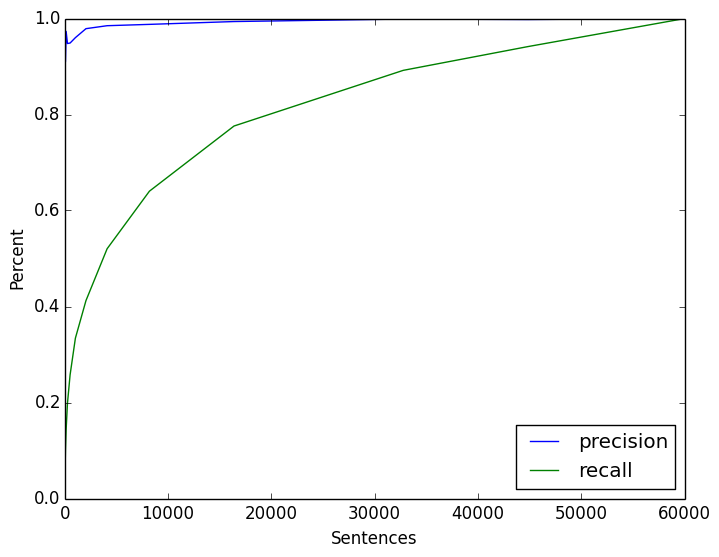
\includegraphics[width=\linewidth, keepaspectratio=true]{figure/precision_recall.png}
  \caption{\small Convergence to the results obtained on the largest run.  Precision relative to that run is very high even for small training sizes.  Recall grows as more link types are observed.}
\end{figure}
We report on the convergence of the results of our ILP with increasing data. With increasing trials of sentences, we measure how similar the subsequent directional assignments would be with each other. Taking the largest run as the answer key, we compared how much the smaller runs deviated from it. 
We recorded the precision of whether the assignments in the smaller runs could be found in those of the largest run, and similarly the recall of whether the assignments in the largest run could be found in the smaller runs. \noteJE{this is not clear.  are we comparing the direction table or the parses?  If the parses, which parses?}

Because the precision values were high, we found that the solutions of the previous runs were consistent with the largest run, and as the data increased so did the recall values, and so we would continue to encounter novel link types and then incorporate them.

\NoteJE{how often is the ``both'' option used?  and how much slack do we have?}

\subsection{English Link-Dependency Analysis}

\begin{figure*}[ht!]
  \centering
  \begin{subfigure}[b]{0.3233\textwidth}
	\begin{dependency}
		\begin{deptext}
			{\scriptsize PR} \& {\scriptsize VB} \& {\scriptsize RB} \& {\scriptsize VB} \& {\scriptsize .} \\
			it \& did \& n't \& work \& . \\
			- \& v-d \& - \& v \& - \\
		\end{deptext}
		\deproot[edge above, edge style = {blue, dotted}]{2}{\small ROOT}
		\depedge[edge below, edge style = {red, ultra thick}]{1}{2}{Ss}
		\depedge[edge above, edge style = {blue, thick}]{2}{1}{\small SBJ}
		\depedge[edge below, edge style = {red, thick}]{2}{3}{N}
		\depedge[edge above, edge style = {blue, thick}]{2}{3}{\small VMOD}
		\depedge[edge below, edge style = {red, thick}]{2}{4}{I*d}
		\depedge[edge above, edge style = {blue, thick}]{2}{4}{\small VC}
		\depedge[edge above, edge style = {blue, dotted}]{2}{5}{\small P}
		\deproot[edge below, edge style = {red, dotted}]{1}{Wd}
		\deproot[edge below, edge style = {orange, ultra thick}]{4}{WV}
		\deproot[edge below, edge style = {red, dotted}]{5}{Xp}
	\end{dependency}
\end{subfigure}
\begin{subfigure}[b]{0.3233\textwidth}
	\begin{dependency}
		\begin{deptext}
			{\scriptsize DT} \& {\scriptsize NN} \& {\scriptsize VB} \& {\scriptsize JJ} \& {\scriptsize .} \\
			the \& reason \& is \& simple \& . \\
			- \& n \& v \& a \& - \\
		\end{deptext}
		\deproot[edge below, edge style = {red, thick}]{3}{WV}
		\deproot[edge above, edge style = {blue, thick}]{3}{\small ROOT}
		\depedge[edge below, edge style = {red, thick}]{3}{2}{Ss*t}
		\depedge[edge above, edge style = {blue, thick}]{3}{2}{\small SBJ}
		\depedge[edge below, edge style = {red, thick}]{3}{4}{Paf}
		\depedge[edge above, edge style = {blue, thick}]{3}{4}{\small VMOD}
		\depedge[edge above, edge style = {blue, dotted}]{3}{5}{\small P}
		\depedge[edge below, edge style = {red, thick}]{2}{1}{D*u}
		\depedge[edge above, edge style = {blue, thick}]{2}{1}{\small NMOD}
		\deproot[edge below, edge style = {orange, ultra thick}]{2}{Wd}
		\deproot[edge below, edge style = {red, dotted}]{5}{Xp}
	\end{dependency}
\end{subfigure}
\begin{subfigure}[b]{0.3233\textwidth}
	\begin{dependency}
		\begin{deptext}
			{\scriptsize DT} \& {\scriptsize NN} \& {\scriptsize VB} \& {\scriptsize RB} \& {\scriptsize .} \\
			the \& judge \& wrote \& again \& . \\
			- \& n \& v-d \& - \& - \\
		\end{deptext}
		\deproot[edge below, edge style = {red, thick}]{3}{WV}
		\deproot[edge above, edge style = {blue, thick}]{3}{\small ROOT}
		\depedge[edge below, edge style = {red, thick}]{3}{2}{Ss}
		\depedge[edge above, edge style = {blue, thick}]{3}{2}{\small SBJ}
		\depedge[edge below, edge style = {red, thick}]{3}{4}{MVa}
		\depedge[edge above, edge style = {blue, thick}]{3}{4}{\small ADV}
		\depedge[edge above, edge style = {blue, dotted}]{3}{5}{\small P}
		\depedge[edge below, edge style = {red, thick}]{2}{1}{Ds}
		\depedge[edge above, edge style = {blue, thick}]{2}{1}{\small NMOD}
		\deproot[edge below, edge style = {orange, ultra thick}]{2}{Wd}
		\deproot[edge below, edge style = {red, dotted}]{5}{Xp}
	\end{dependency}
\end{subfigure}


  \caption{\small Example Parses: The top blue arcs represent conll dependencies; the bottom red arcs represent directionalized link grammar parses. See the Appendix for more details.}
  \label{fig:parses}
\end{figure*}

In the case of English, we had manually produced  single-headed 
 CoNLL annotations \cite{!!!}.

Using the sentences of the dependency corpus as comparison, we find that the link parses do not wholly subsume dependency parses, and that the undirected links match roughly three fourths of the arcs in the conll dependency corpus. \todo{This is because...} 

\begin{figure}[ht!]
  \centering
  \small
  	\begin{tabular}{|l|l|l|}
		\hline
		 & CoNLL arcs & Percent of total \\ 
		\hline
		Matches: & 64165 & 64.86\%\\ 
		\hline
		Flipped direction: & 4430 & 4.48\%\\ 
		\hline
		Mismatches: & 30334 & 30.66\%\\ 
		\hline
		Total: & 98929 & 100\% \\ 
		\hline
	\end{tabular}

  \caption{Arcs that match links}
\end{figure}

we measure whether the direction we chose is the same as the original dependency data.  Finally, we look to see that given a link label, whether the original conll label can be recovered.

Of the sentences with complete parses, about 78.10\%
\noteJE{why ``about''?}
had at least one multiheaded word.

\NoteJE{discuss linguistic differences!}

\NoteJE{what do we say about Russian?}


\section{Discussion}



\todo{more in the appendix ...}

\NoteJE{We should acknowledge that another option would be to post-process either CoNLL parses or our link parses to automatically add more multi-heading, e.g., to handle control phenomena ("John wants to skip" or "Jane ran for office in order to change the tax laws" should have John/Jane be the subject of two verbs).  However, that requires per-language}

We have a set of 100 parses similar to figure~\ref{fig:parses} in the appendix.


\section{Future Work}

\subsection{Slack Hierarchy}
We would like to introduce slack on the link grammar types such that link types with the same coarse grained label would try and align the same way as the majority in the group, where the preceding capital letters of the link type denote the coarse grained label, while the subscript letters denote further information. This slack would place a prior on rare or never-before seen link types to be assigned in the same way as other similar link types. We think that this will give the ILP better flexibility to handle noise and novel link types while still trying to learn the overall link grammar.





\section{Related Work}



\bibliographystyle{acl2014}
\bibliography{LinksToDAG}





\clearpage
\appendix
\section{ILP Formulation}
We present our ILP formulation. 

\begin{figure}[!htb]
  \small
  \begin{align*}
    \text{Sets:}&&\\
    &\textsc{link}_{\textsc{sentence},\textsc{label}, i,j} \in \textsc{links} &\\
    &\textsc{label} \in \textsc{labels}&\\ 
    &\textsc{dir} = \{\textsc{left}, \textsc{right}\} &\\
    \text{Params:}&&\\
    &\textsc{m}_\textsc{length} = \max (\forall{\textsc{link}_{\textsc{sentence}, i,j}} \max(i,j)) &\\
    %&\textsc{count}_{\textsc{label}, \textsc{dir}} = \sum_{\textsc{link}_{\textsc{label},\textsc{dir}}}1 &\\
    &\textsc{cost}_{\textsc{label}} = \frac{100}{ \sum_{\textsc{link}_{\textsc{label},\textsc{dir}}}1 } &\\
    \text{Variables:}&&\\
    &\textsc{slack}_{\textsc{link}} \geq 0 &\\ 
    &\textsc{depth}_{\textsc{sentence},i} \geq 0 &\\
    &\textsc{allowed}_{\textsc{label},\textsc{dir}} = \{0,1\}&\\
    &\textsc{arc}_{\textsc{link}} = \{0,1\} &\\
    \text{minimize:}& &\\ 
    &\sum_{\textsc{label}, \textsc{dir}} (\textsc{allowed}_{\textsc{label},\textsc{dir}}) + \textsc{cost}_{\textsc{label}} \cdot \sum_\textsc{link} \textsc{slack}_{\textsc{link}} &\\
    &&\\
    \text{subject to: }& &\\
    &\text{Links go in the allowed directions, except for slack}&\\
    &\forall{\textsc{link}_{i,j,\textsc{label}}}: 1-\textsc{arc}_{\textsc{link}} \leq \textsc{allowed}_{\textsc{label}, \textsc{left}} + \textsc{slack}_{\textsc{link}} &\\
    &\forall{\textsc{link}_{i,j,\textsc{label}}}: \textsc{arc}_{\textsc{link}} \leq \textsc{allowed}_{\textsc{label}, \textsc{right}} + \textsc{slack}_{\textsc{link}} &\\
    &\text{Depth constraints for acyclicity}&\\
    &\forall{\textsc{link}_{\textsc{sentence},i}}: \textsc{depth}_{\textsc{sentence},\text{root}} \leq \textsc{depth}_{\textsc{sentence},i} &\\
    &\forall{\textsc{link}_{\textsc{sentence},i,j}}: \textsc{depth}_{\textsc{sentence},i} + \textsc{m}_\textsc{length}\cdot\textsc{arc}_{\textsc{sentence},i,j} \geq \textsc{depth}_{\textsc{sentence},j} + 1 &\\
    &\forall{\textsc{link}_{\textsc{sentence},i,j}}: \textsc{depth}_{\textsc{sentence},j} + \textsc{m}_\textsc{length}\cdot(1-\textsc{arc}_{\textsc{sentence},i,j}) \geq \textsc{depth}_{\textsc{sentence},i} + 1 &\\
    &\text{Every token has a parent}&\\
    &\forall{\textsc{link}_{\textsc{sentence},i \neq \textsc{root}}}: \sum_{\textsc{link}_{\textsc{sentence},i,j}} (1-\textsc{arc}_{\textsc{sentence},i,j}) + \sum_{\textsc{link}_{\textsc{sentence},j,i}}(\textsc{arc}_{\textsc{sentence},j,i}) \geq 1&\\
  \end{align*}
  \caption{\small The ILP formulation.}
\end{figure}


\clearpage

\section{English Link Types}

\todo[inline]{A table here that lists each link grammar type together with its
  count, its allowed direction(s), its percentage of majority
  directions by token, and its most common corresponding CoNLL tags
  with percentages.  Readers could cut-and-paste this data to make a 
  cheap post-processor for LG parses.}



\begin{figure*}
\begin{tabular}{|l|l|l|l||l|l|}
\hline
Label & Count & Left & Right & CoNLL & CoNLL Percentage\\ 
\hline
 A & 3980 & 0\% (0) & 100\% (3980) & NMOD & 97\% (3253/3336) \\ 
\hline
 AA & 3 & 0\% (0) & 100\% (3) & - &  \\ 
\hline
 AF & 5 & 60\% (3) & 40\% (2) & ADV & 100\% (1/1) \\ 
\hline
 AFd & 6 & 100\% (6) & 0\% (0) & VMOD & 100\% (4/4) \\ 
\hline
 AFh & 1 & 100\% (1) & 0\% (0) & - &  \\ 
\hline
 AJla & 65 & 0\% (0) & 100\% (65) & COORD & 92\% (49/53) \\ 
\hline
 AJlc & 8 & 0\% (0) & 100\% (8) & COORD & 100\% (7/7) \\ 
\hline
 AJls & 1 & 0\% (0) & 100\% (1) & COORD & 100\% (1/1) \\ 
\hline
 AJn & 2 & 0\% (0) & 100\% (2) & COORD & 100\% (2/2) \\ 
\hline
 AJra & 65 & 100\% (65) & 0\% (0) & COORD & 100\% (55/55) \\ 
\hline
 AJrc & 10 & 100\% (10) & 0\% (0) & COORD & 100\% (6/6) \\ 
\hline
 AJrs & 1 & 100\% (1) & 0\% (0) & COORD & 100\% (1/1) \\ 
\hline
 AL & 6 & 100\% (6) & 0\% (0) & - &  \\ 
\hline
 ALx & 34 & 100\% (34) & 0\% (0) & - &  \\ 
\hline
 AM & 15 & 0\% (0) & 100\% (15) & AMOD & 83\% (5/6) \\ 
\hline
 AN & 5249 & 0\% (0) & 100\% (5249) & NMOD & 96\% (4221/4366) \\ 
\hline
 AZ & 2 & 100\% (2) & 0\% (0) & ADV & 100\% (2/2) \\ 
\hline
 Ah & 563 & 0\% (0) & 100\% (563) & NMOD & 99\% (461/462) \\ 
\hline
 Am & 123 & 0\% (0) & 100\% (123) & NMOD & 98\% (98/99) \\ 
\hline
 B & 18 & 100\% (18) & 0\% (0) & NMOD & 50\% (3/6) \\ 
\hline
 B**t & 12 & 100\% (12) & 0\% (0) & SBJ & 60\% (3/5) \\ 
\hline
 B*d & 75 & 100\% (75) & 0\% (0) & AMOD & 48\% (19/39) \\ 
\hline
 B*w & 10 & 100\% (10) & 0\% (0) & OBJ & 50\% (3/6) \\ 
\hline
 BIh & 5 & 100\% (5) & 0\% (0) & ADV & 100\% (1/1) \\ 
\hline
 BIq & 4 & 100\% (4) & 0\% (0) & - &  \\ 
\hline
 BIqd & 3 & 100\% (3) & 0\% (0) & - &  \\ 
\hline
 BIt & 9 & 100\% (9) & 0\% (0) & VMOD & 100\% (7/7) \\ 
\hline
 Bcd & 2 & 100\% (2) & 0\% (0) & PMOD & 50\% (1/2) \\ 
\hline
 Bp & 182 & 100\% (182) & 0\% (0) & NMOD & 98\% (125/127) \\ 
\hline
 Bp*t & 29 & 100\% (29) & 0\% (0) & NMOD & 77\% (7/9) \\ 
\hline
 Bpd & 87 & 100\% (87) & 0\% (0) & NMOD & 72\% (21/29) \\ 
\hline
 Bpj & 4 & 100\% (4) & 0\% (0) & - &  \\ 
\hline
 Bpm & 3 & 100\% (3) & 0\% (0) & OBJ & 100\% (1/1) \\ 
\hline
 Bpw & 2 & 100\% (2) & 0\% (0) & NMOD & 100\% (1/1) \\ 
\hline
 Bs & 189 & 100\% (189) & 0\% (0) & NMOD & 98\% (125/127) \\ 
\hline
 Bs*t & 41 & 100\% (41) & 0\% (0) & NMOD & 85\% (12/14) \\ 
\hline
 Bsd & 165 & 100\% (165) & 0\% (0) & NMOD & 53\% (36/67) \\ 
\hline
 Bsdt & 1 & 100\% (1) & 0\% (0) & SBJ & 100\% (1/1) \\ 
\hline
 Bsj & 1 & 100\% (1) & 0\% (0) & - &  \\ 
\hline
 Bsm & 7 & 85\% (6) & 14\% (1) & OBJ & 60\% (3/5) \\ 
\hline
 Bsmt & 1 & 100\% (1) & 0\% (0) & - &  \\ 
\hline
 Bsw & 12 & 100\% (12) & 0\% (0) & OBJ & 50\% (2/4) \\ 
\hline
 Bswt & 1 & 100\% (1) & 0\% (0) & VMOD & 100\% (1/1) \\ 
\hline
 CC & 92 & 100\% (92) & 0\% (0) & PRN & 60\% (6/10) \\ 
\hline
 CCq & 2 & 100\% (2) & 0\% (0) & - &  \\ 
\hline
 CO & 932 & 0\% (0) & 100\% (932) & NMOD & 30\% (15/49) \\ 
\hline
 CO*n & 46 & 0\% (0) & 100\% (46) & DEP & 100\% (1/1) \\ 
\hline
 CO*s & 141 & 0\% (0) & 100\% (141) & VMOD & 100\% (1/1) \\ 
\hline
 COa & 45 & 0\% (0) & 100\% (45) & NMOD & 87\% (7/8) \\ 
\hline
 COd & 37 & 0\% (0) & 100\% (37) & NMOD & 100\% (4/4) \\ 
\hline
\end{tabular}
\end{figure*}
\begin{figure*}
\begin{tabular}{|l|l|l|l||l|l|}
\hline
Label & Count & Left & Right & CoNLL & CoNLL Percentage\\ 
\hline
 COdn & 1 & 0\% (0) & 100\% (1) & - &  \\ 
\hline
 COds & 5 & 0\% (0) & 100\% (5) & - &  \\ 
\hline
 COp & 84 & 0\% (0) & 100\% (84) & - &  \\ 
\hline
 COq & 16 & 0\% (0) & 100\% (16) & - &  \\ 
\hline
 CP & 149 & 100\% (149) & 0\% (0) & ROOT & 100\% (131/131) \\ 
\hline
 CPx & 13 & 100\% (13) & 0\% (0) & ROOT & 100\% (11/11) \\ 
\hline
 CQ & 6 & 100\% (6) & 0\% (0) & VMOD & 66\% (4/6) \\ 
\hline
 CV & 1799 & 100\% (1799) & 0\% (0) & VMOD & 51\% (516/1003) \\ 
\hline
 CX & 5 & 100\% (5) & 0\% (0) & VMOD & 75\% (3/4) \\ 
\hline
 Ca & 8 & 100\% (8) & 0\% (0) & - &  \\ 
\hline
 Cc & 6 & 100\% (6) & 0\% (0) & AMOD & 100\% (1/1) \\ 
\hline
 Ce & 659 & 100\% (659) & 0\% (0) & OBJ & 40\% (9/22) \\ 
\hline
 Cet & 379 & 100\% (379) & 0\% (0) & SBJ & 33\% (1/3) \\ 
\hline
 Ci & 1 & 100\% (1) & 0\% (0) & - &  \\ 
\hline
 Cr & 76 & 100\% (76) & 0\% (0) & SBJ & 100\% (1/1) \\ 
\hline
 Cs & 676 & 100\% (676) & 0\% (0) & PMOD & 60\% (12/20) \\ 
\hline
 Ct & 2 & 100\% (2) & 0\% (0) & - &  \\ 
\hline
 Cta & 6 & 100\% (6) & 0\% (0) & VMOD & 100\% (1/1) \\ 
\hline
 D & 139 & 0\% (1) & 99\% (138) & NMOD & 100\% (76/76) \\ 
\hline
 D**w & 2 & 100\% (2) & 0\% (0) & NMOD & 100\% (1/1) \\ 
\hline
 D**y & 1 & 0\% (0) & 100\% (1) & NMOD & 100\% (1/1) \\ 
\hline
 D*u & 342 & 0\% (0) & 100\% (342) & NMOD & 100\% (270/270) \\ 
\hline
 D*un & 8 & 0\% (0) & 100\% (8) & AMOD & 62\% (5/8) \\ 
\hline
 D*uw & 1 & 100\% (1) & 0\% (0) & NMOD & 100\% (1/1) \\ 
\hline
 D*uy & 7 & 0\% (0) & 100\% (7) & NMOD & 100\% (7/7) \\ 
\hline
 DD & 349 & 0\% (0) & 100\% (349) & NMOD & 100\% (87/87) \\ 
\hline
 DG & 537 & 0\% (0) & 100\% (537) & NMOD & 100\% (486/486) \\ 
\hline
 DP & 7 & 0\% (0) & 100\% (7) & SBJ & 100\% (1/1) \\ 
\hline
 DTa & 2 & 0\% (0) & 100\% (2) & NMOD & 100\% (2/2) \\ 
\hline
 DTi & 146 & 0\% (0) & 100\% (146) & NMOD & 98\% (144/146) \\ 
\hline
 DTie & 23 & 0\% (0) & 100\% (23) & NMOD & 100\% (22/22) \\ 
\hline
 DTn & 115 & 0\% (0) & 100\% (115) & NMOD & 100\% (115/115) \\ 
\hline
 Dm & 1 & 0\% (0) & 100\% (1) & - &  \\ 
\hline
 Dmc & 2107 & 0\% (2) & 99\% (2105) & NMOD & 99\% (1665/1667) \\ 
\hline
 Dmck & 51 & 0\% (0) & 100\% (51) & NMOD & 100\% (47/47) \\ 
\hline
 Dmcm & 25 & 0\% (0) & 100\% (25) & NMOD & 100\% (21/21) \\ 
\hline
 Dmcn & 514 & 0\% (0) & 100\% (514) & NMOD & 99\% (414/416) \\ 
\hline
 Dmcw & 10 & 100\% (10) & 0\% (0) & NMOD & 80\% (8/10) \\ 
\hline
 Dmcy & 4 & 0\% (0) & 100\% (4) & NMOD & 100\% (2/2) \\ 
\hline
 Dmu & 1182 & 0\% (0) & 100\% (1182) & NMOD & 100\% (948/948) \\ 
\hline
 Dmuk & 13 & 0\% (0) & 100\% (13) & NMOD & 100\% (12/12) \\ 
\hline
 Dmum & 30 & 0\% (0) & 100\% (30) & NMOD & 100\% (24/24) \\ 
\hline
 Dmuw & 1 & 100\% (1) & 0\% (0) & - &  \\ 
\hline
 Dmuy & 2 & 0\% (0) & 100\% (2) & NMOD & 100\% (2/2) \\ 
\hline
 Dn & 6 & 0\% (0) & 100\% (6) & NMOD & 100\% (1/1) \\ 
\hline
 Ds & 6029 & 0\% (0) & 100\% (6029) & NMOD & 100\% (5369/5369) \\ 
\hline
 Ds*k & 30 & 0\% (0) & 100\% (30) & NMOD & 100\% (29/29) \\ 
\hline
 Ds*w & 16 & 100\% (16) & 0\% (0) & NMOD & 100\% (14/14) \\ 
\hline
 Ds*y & 5 & 0\% (0) & 100\% (5) & NMOD & 100\% (5/5) \\ 
\hline
 Dsu & 263 & 0\% (0) & 100\% (263) & NMOD & 100\% (252/252) \\ 
\hline
\end{tabular}
\end{figure*}
\begin{figure*}
\begin{tabular}{|l|l|l|l||l|l|}
\hline
Label & Count & Left & Right & CoNLL & CoNLL Percentage\\ 
\hline
 Dsuk & 2 & 0\% (0) & 100\% (2) & NMOD & 100\% (2/2) \\ 
\hline
 E & 750 & 0\% (0) & 100\% (750) & ADV & 93\% (457/488) \\ 
\hline
 EA & 158 & 0\% (0) & 100\% (158) & AMOD & 94\% (127/134) \\ 
\hline
 EAh & 2 & 100\% (2) & 0\% (0) & AMOD & 100\% (2/2) \\ 
\hline
 EAm & 62 & 0\% (0) & 100\% (62) & AMOD & 97\% (47/48) \\ 
\hline
 EAx & 1 & 0\% (0) & 100\% (1) & AMOD & 100\% (1/1) \\ 
\hline
 EAxk & 20 & 0\% (0) & 100\% (20) & AMOD & 100\% (18/18) \\ 
\hline
 EAy & 24 & 0\% (0) & 100\% (24) & AMOD & 87\% (14/16) \\ 
\hline
 EBb & 10 & 100\% (10) & 0\% (0) & COORD & 75\% (3/4) \\ 
\hline
 EBm & 196 & 100\% (196) & 0\% (0) & VMOD & 60\% (93/153) \\ 
\hline
 EBmm & 2 & 100\% (2) & 0\% (0) & - &  \\ 
\hline
 EBmy & 1 & 100\% (1) & 0\% (0) & - &  \\ 
\hline
 EBx & 64 & 100\% (64) & 0\% (0) & P & 100\% (11/11) \\ 
\hline
 EBxy & 1 & 100\% (1) & 0\% (0) & - &  \\ 
\hline
 EBy & 1 & 0\% (0) & 100\% (1) & COORD & 100\% (1/1) \\ 
\hline
 ECa & 39 & 0\% (0) & 100\% (39) & AMOD & 97\% (33/34) \\ 
\hline
 ECn & 4 & 0\% (0) & 100\% (4) & AMOD & 66\% (2/3) \\ 
\hline
 ECx & 5 & 0\% (0) & 100\% (5) & AMOD & 100\% (2/2) \\ 
\hline
 EE & 8 & 0\% (0) & 100\% (8) & AMOD & 100\% (6/6) \\ 
\hline
 EEh & 8 & 100\% (8) & 0\% (0) & AMOD & 87\% (7/8) \\ 
\hline
 EEm & 9 & 0\% (0) & 100\% (9) & AMOD & 100\% (7/7) \\ 
\hline
 EEx & 5 & 0\% (0) & 100\% (5) & NMOD & 80\% (4/5) \\ 
\hline
 EExk & 12 & 0\% (0) & 100\% (12) & AMOD & 100\% (12/12) \\ 
\hline
 EEy & 18 & 0\% (0) & 100\% (18) & AMOD & 94\% (16/17) \\ 
\hline
 EF & 5 & 100\% (5) & 0\% (0) & AMOD & 100\% (5/5) \\ 
\hline
 EI & 4 & 0\% (0) & 100\% (4) & PMOD & 100\% (1/1) \\ 
\hline
 EL & 1 & 100\% (1) & 0\% (0) & NMOD & 100\% (1/1) \\ 
\hline
 EN & 247 & 0\% (0) & 100\% (247) & AMOD & 90\% (180/199) \\ 
\hline
 EW & 1 & 0\% (0) & 100\% (1) & - &  \\ 
\hline
 EZ & 5 & 0\% (0) & 100\% (5) & - &  \\ 
\hline
 Ec & 19 & 0\% (0) & 100\% (19) & AMOD & 100\% (12/12) \\ 
\hline
 Em & 224 & 0\% (0) & 100\% (224) & ADV & 75\% (144/190) \\ 
\hline
 Eq & 22 & 0\% (0) & 100\% (22) & PRN & 90\% (19/21) \\ 
\hline
 FM & 3 & 100\% (3) & 0\% (0) & PMOD & 100\% (3/3) \\ 
\hline
 G & 3447 & 0\% (0) & 100\% (3447) & NMOD & 90\% (2184/2414) \\ 
\hline
 GN & 147 & 0\% (0) & 100\% (147) & NMOD & 100\% (132/132) \\ 
\hline
 H & 3 & 100\% (3) & 0\% (0) & NMOD & 66\% (2/3) \\ 
\hline
 HA & 3 & 0\% (0) & 100\% (3) & - &  \\ 
\hline
 I & 2207 & 99\% (2204) & 0\% (3) & VMOD & 63\% (1337/2108) \\ 
\hline
 I*d & 120 & 100\% (120) & 0\% (0) & VC & 93\% (105/112) \\ 
\hline
 I*g & 1 & 100\% (1) & 0\% (0) & - &  \\ 
\hline
 I*j & 25 & 100\% (25) & 0\% (0) & OBJ & 61\% (11/18) \\ 
\hline
 I*v & 52 & 100\% (52) & 0\% (0) & VC & 39\% (13/33) \\ 
\hline
 IDBAA & 6 & 0\% (0) & 100\% (6) & PRT & 100\% (6/6) \\ 
\hline
 IDBAI & 1 & 0\% (0) & 100\% (1) & ADV & 100\% (1/1) \\ 
\hline
 IDBBB & 1 & 0\% (0) & 100\% (1) & ADV & 100\% (1/1) \\ 
\hline
 IDBCM & 1 & 0\% (0) & 100\% (1) & PRT & 100\% (1/1) \\ 
\hline
 IDBDQ & 1 & 0\% (0) & 100\% (1) & AMOD & 100\% (1/1) \\ 
\hline
 IDBDS & 1 & 0\% (0) & 100\% (1) & - &  \\ 
\hline
 IDBDX & 1 & 0\% (0) & 100\% (1) & AMOD & 100\% (1/1) \\ 
\hline
\end{tabular}
\end{figure*}
\begin{figure*}
\begin{tabular}{|l|l|l|l||l|l|}
\hline
Label & Count & Left & Right & CoNLL & CoNLL Percentage\\ 
\hline
 IDBDY & 27 & 0\% (0) & 100\% (27) & PMOD & 77\% (21/27) \\ 
\hline
 IDBEA & 5 & 0\% (0) & 100\% (5) & AMOD & 100\% (5/5) \\ 
\hline
 IDBEB & 3 & 0\% (0) & 100\% (3) & AMOD & 100\% (3/3) \\ 
\hline
 IDBEC & 1 & 0\% (0) & 100\% (1) & PMOD & 100\% (1/1) \\ 
\hline
 IDBED & 14 & 0\% (0) & 100\% (14) & DEP & 57\% (8/14) \\ 
\hline
 IDBEE & 1 & 0\% (0) & 100\% (1) & DEP & 100\% (1/1) \\ 
\hline
 IDBEF & 2 & 0\% (0) & 100\% (2) & AMOD & 100\% (2/2) \\ 
\hline
 IDBEG & 9 & 0\% (0) & 100\% (9) & DEP & 77\% (7/9) \\ 
\hline
 IDBEH & 11 & 0\% (0) & 100\% (11) & - &  \\ 
\hline
 IDBEI & 11 & 0\% (0) & 100\% (11) & AMOD & 100\% (11/11) \\ 
\hline
 IDBEJ & 6 & 0\% (0) & 100\% (6) & NMOD & 100\% (6/6) \\ 
\hline
 IDBEK & 6 & 0\% (0) & 100\% (6) & PMOD & 100\% (6/6) \\ 
\hline
 IDBEL & 1 & 0\% (0) & 100\% (1) & NMOD & 100\% (1/1) \\ 
\hline
 IDBEN & 1 & 0\% (0) & 100\% (1) & PMOD & 100\% (1/1) \\ 
\hline
 IDBEQ & 53 & 0\% (0) & 100\% (53) & PMOD & 100\% (53/53) \\ 
\hline
 IDBET & 6 & 0\% (0) & 100\% (6) & NMOD & 100\% (6/6) \\ 
\hline
 IDBEU & 6 & 0\% (0) & 100\% (6) & PMOD & 100\% (6/6) \\ 
\hline
 IDBEV & 7 & 0\% (0) & 100\% (7) & AMOD & 83\% (5/6) \\ 
\hline
 IDBEW & 4 & 0\% (0) & 100\% (4) & AMOD & 50\% (2/4) \\ 
\hline
 IDBEX & 1 & 0\% (0) & 100\% (1) & PMOD & 100\% (1/1) \\ 
\hline
 IDBEZ & 2 & 0\% (0) & 100\% (2) & AMOD & 100\% (2/2) \\ 
\hline
 IDBFA & 3 & 0\% (0) & 100\% (3) & PMOD & 100\% (3/3) \\ 
\hline
 IDBFD & 3 & 0\% (0) & 100\% (3) & PMOD & 100\% (3/3) \\ 
\hline
 IDBFF & 2 & 0\% (0) & 100\% (2) & PMOD & 100\% (2/2) \\ 
\hline
 IDBFG & 15 & 0\% (0) & 100\% (15) & AMOD & 100\% (15/15) \\ 
\hline
 IDBFH & 1 & 0\% (0) & 100\% (1) & PMOD & 100\% (1/1) \\ 
\hline
 IDBFI & 3 & 0\% (0) & 100\% (3) & PMOD & 100\% (3/3) \\ 
\hline
 IDBFJ & 2 & 0\% (0) & 100\% (2) & PMOD & 100\% (2/2) \\ 
\hline
 IDBFK & 46 & 0\% (0) & 100\% (46) & DEP & 100\% (46/46) \\ 
\hline
 IDBFO & 2 & 0\% (0) & 100\% (2) & PMOD & 50\% (1/2) \\ 
\hline
 IDBFP & 2 & 0\% (0) & 100\% (2) & NMOD & 100\% (2/2) \\ 
\hline
 IDBFQ & 2 & 0\% (0) & 100\% (2) & PMOD & 100\% (2/2) \\ 
\hline
 IDBFT & 1 & 0\% (0) & 100\% (1) & NMOD & 100\% (1/1) \\ 
\hline
 IDBFU & 1 & 0\% (0) & 100\% (1) & PMOD & 100\% (1/1) \\ 
\hline
 IDBFV & 1 & 0\% (0) & 100\% (1) & AMOD & 100\% (1/1) \\ 
\hline
 IDBFY & 1 & 0\% (0) & 100\% (1) & AMOD & 100\% (1/1) \\ 
\hline
 IDBGB & 1 & 0\% (0) & 100\% (1) & NMOD & 100\% (1/1) \\ 
\hline
 IDBGC & 1 & 0\% (0) & 100\% (1) & PMOD & 100\% (1/1) \\ 
\hline
 IDBGK & 7 & 0\% (0) & 100\% (7) & AMOD & 100\% (5/5) \\ 
\hline
 IDBGV & 1 & 0\% (0) & 100\% (1) & PMOD & 100\% (1/1) \\ 
\hline
 IDBHF & 1 & 0\% (0) & 100\% (1) & PMOD & 100\% (1/1) \\ 
\hline
 IDBHL & 1 & 0\% (0) & 100\% (1) & PMOD & 100\% (1/1) \\ 
\hline
 IDBHQ & 1 & 0\% (0) & 100\% (1) & PMOD & 100\% (1/1) \\ 
\hline
 IDBHS & 1 & 0\% (0) & 100\% (1) & PMOD & 100\% (1/1) \\ 
\hline
 IDBIA & 2 & 0\% (0) & 100\% (2) & PMOD & 100\% (2/2) \\ 
\hline
 IDBIB & 2 & 0\% (0) & 100\% (2) & PMOD & 100\% (2/2) \\ 
\hline
 IDBIC & 1 & 0\% (0) & 100\% (1) & AMOD & 100\% (1/1) \\ 
\hline
 IDBIE & 2 & 0\% (0) & 100\% (2) & PMOD & 100\% (2/2) \\ 
\hline
 IDBIF & 2 & 0\% (0) & 100\% (2) & PMOD & 100\% (2/2) \\ 
\hline
 IDBIG & 2 & 0\% (0) & 100\% (2) & PMOD & 100\% (2/2) \\ 
\hline
\end{tabular}
\end{figure*}
\begin{figure*}
\begin{tabular}{|l|l|l|l||l|l|}
\hline
Label & Count & Left & Right & CoNLL & CoNLL Percentage\\ 
\hline
 IDBIT & 1 & 0\% (0) & 100\% (1) & PMOD & 100\% (1/1) \\ 
\hline
 IDBJN & 1 & 0\% (0) & 100\% (1) & PMOD & 100\% (1/1) \\ 
\hline
 IDBKO & 1 & 0\% (0) & 100\% (1) & PMOD & 100\% (1/1) \\ 
\hline
 IDBKU & 3 & 0\% (0) & 100\% (3) & NMOD & 100\% (3/3) \\ 
\hline
 IDBKY & 1 & 0\% (0) & 100\% (1) & NMOD & 100\% (1/1) \\ 
\hline
 IDBLC & 2 & 0\% (0) & 100\% (2) & - &  \\ 
\hline
 IDBLD & 1 & 0\% (0) & 100\% (1) & - &  \\ 
\hline
 IDBLE & 2 & 0\% (0) & 100\% (2) & - &  \\ 
\hline
 IDBLF & 1 & 0\% (0) & 100\% (1) & NMOD & 100\% (1/1) \\ 
\hline
 IDBLG & 1 & 0\% (0) & 100\% (1) & - &  \\ 
\hline
 IDBLH & 1 & 0\% (0) & 100\% (1) & COORD & 100\% (1/1) \\ 
\hline
 IDBLI & 1 & 0\% (0) & 100\% (1) & NMOD & 100\% (1/1) \\ 
\hline
 IDBLP & 1 & 0\% (0) & 100\% (1) & NMOD & 100\% (1/1) \\ 
\hline
 IDBLS & 2 & 0\% (0) & 100\% (2) & NMOD & 100\% (2/2) \\ 
\hline
 IDBLZ & 2 & 0\% (0) & 100\% (2) & NMOD & 100\% (2/2) \\ 
\hline
 IDBNL & 1 & 0\% (0) & 100\% (1) & - &  \\ 
\hline
 IDBNW & 1 & 0\% (0) & 100\% (1) & - &  \\ 
\hline
 IDBNY & 4 & 0\% (0) & 100\% (4) & - &  \\ 
\hline
 IDBNZ & 1 & 0\% (0) & 100\% (1) & - &  \\ 
\hline
 IDBOA & 1 & 0\% (0) & 100\% (1) & - &  \\ 
\hline
 IDBOD & 1 & 0\% (0) & 100\% (1) & - &  \\ 
\hline
 IDBOF & 1 & 0\% (0) & 100\% (1) & - &  \\ 
\hline
 IDBOI & 1 & 0\% (0) & 100\% (1) & - &  \\ 
\hline
 IDBOM & 1 & 0\% (0) & 100\% (1) & - &  \\ 
\hline
 IDBOZ & 4 & 0\% (0) & 100\% (4) & COORD & 100\% (2/2) \\ 
\hline
 IDBPA & 9 & 0\% (0) & 100\% (9) & P & 100\% (3/3) \\ 
\hline
 IDBPI & 1 & 0\% (0) & 100\% (1) & NMOD & 100\% (1/1) \\ 
\hline
 IDBSF & 1 & 0\% (0) & 100\% (1) & PMOD & 100\% (1/1) \\ 
\hline
 IDBTZ & 2 & 0\% (0) & 100\% (2) & VMOD & 100\% (2/2) \\ 
\hline
 IDBUB & 3 & 0\% (0) & 100\% (3) & VMOD & 100\% (3/3) \\ 
\hline
 IDBUI & 3 & 0\% (0) & 100\% (3) & PMOD & 100\% (2/2) \\ 
\hline
 IDBUQ & 2 & 0\% (0) & 100\% (2) & NMOD & 100\% (1/1) \\ 
\hline
 IDBUW & 6 & 0\% (0) & 100\% (6) & AMOD & 100\% (3/3) \\ 
\hline
 IDBUX & 6 & 0\% (0) & 100\% (6) & - &  \\ 
\hline
 IDBUY & 4 & 0\% (0) & 100\% (4) & AMOD & 100\% (3/3) \\ 
\hline
 IDBUZ & 6 & 0\% (0) & 100\% (6) & AMOD & 100\% (5/5) \\ 
\hline
 IDBVA & 2 & 0\% (0) & 100\% (2) & - &  \\ 
\hline
 IDBVB & 4 & 0\% (0) & 100\% (4) & AMOD & 100\% (4/4) \\ 
\hline
 IDBVC & 4 & 0\% (0) & 100\% (4) & - &  \\ 
\hline
 IDBVD & 1 & 0\% (0) & 100\% (1) & - &  \\ 
\hline
 IDBVE & 1 & 0\% (0) & 100\% (1) & - &  \\ 
\hline
 IDBVF & 1 & 0\% (0) & 100\% (1) & AMOD & 100\% (1/1) \\ 
\hline
 IDBVG & 28 & 0\% (0) & 100\% (28) & AMOD & 88\% (22/25) \\ 
\hline
 IDBVH & 29 & 0\% (0) & 100\% (29) & AMOD & 96\% (25/26) \\ 
\hline
 IDBVI & 1 & 0\% (0) & 100\% (1) & AMOD & 100\% (1/1) \\ 
\hline
 IDBVK & 20 & 0\% (0) & 100\% (20) & NMOD & 100\% (2/2) \\ 
\hline
 IDBVL & 3 & 0\% (0) & 100\% (3) & AMOD & 100\% (3/3) \\ 
\hline
 IDBVQ & 5 & 0\% (0) & 100\% (5) & NMOD & 100\% (5/5) \\ 
\hline
 IDBVW & 3 & 0\% (0) & 100\% (3) & AMOD & 100\% (3/3) \\ 
\hline
 IDBWG & 1 & 0\% (0) & 100\% (1) & PMOD & 100\% (1/1) \\ 
\hline
\end{tabular}
\end{figure*}
\begin{figure*}
\begin{tabular}{|l|l|l|l||l|l|}
\hline
Label & Count & Left & Right & CoNLL & CoNLL Percentage\\ 
\hline
 IDBWI & 1 & 0\% (0) & 100\% (1) & PMOD & 100\% (1/1) \\ 
\hline
 IDBWU & 1 & 0\% (0) & 100\% (1) & PMOD & 100\% (1/1) \\ 
\hline
 IDBXB & 1 & 0\% (0) & 100\% (1) & PMOD & 100\% (1/1) \\ 
\hline
 IDBXC & 1 & 0\% (0) & 100\% (1) & PMOD & 100\% (1/1) \\ 
\hline
 IDBXK & 1 & 0\% (0) & 100\% (1) & PMOD & 100\% (1/1) \\ 
\hline
 IDBXN & 1 & 0\% (0) & 100\% (1) & PMOD & 100\% (1/1) \\ 
\hline
 IDBXW & 1 & 0\% (0) & 100\% (1) & NMOD & 100\% (1/1) \\ 
\hline
 IDBXX & 1 & 0\% (0) & 100\% (1) & - &  \\ 
\hline
 IDBYD & 1 & 0\% (0) & 100\% (1) & PMOD & 100\% (1/1) \\ 
\hline
 IDBYG & 1 & 0\% (0) & 100\% (1) & AMOD & 100\% (1/1) \\ 
\hline
 IDCBA & 1 & 0\% (0) & 100\% (1) & NMOD & 100\% (1/1) \\ 
\hline
 IDCBB & 1 & 0\% (0) & 100\% (1) & VMOD & 100\% (1/1) \\ 
\hline
 IDCBD & 21 & 0\% (0) & 100\% (21) & PMOD & 100\% (21/21) \\ 
\hline
 IDCBE & 8 & 0\% (0) & 100\% (8) & PMOD & 100\% (8/8) \\ 
\hline
 IDCBF & 8 & 0\% (0) & 100\% (8) & PMOD & 100\% (8/8) \\ 
\hline
 IDCBG & 1 & 0\% (0) & 100\% (1) & PMOD & 100\% (1/1) \\ 
\hline
 IDCBH & 5 & 0\% (0) & 100\% (5) & PMOD & 100\% (5/5) \\ 
\hline
 IDCBX & 1 & 0\% (0) & 100\% (1) & NMOD & 100\% (1/1) \\ 
\hline
 IDCCI & 1 & 0\% (0) & 100\% (1) & PMOD & 100\% (1/1) \\ 
\hline
 IDCDB & 1 & 0\% (0) & 100\% (1) & AMOD & 100\% (1/1) \\ 
\hline
 IDCDR & 1 & 0\% (0) & 100\% (1) & - &  \\ 
\hline
 IDCDT & 1 & 0\% (0) & 100\% (1) & PMOD & 100\% (1/1) \\ 
\hline
 IDCDU & 10 & 0\% (0) & 100\% (10) & AMOD & 100\% (10/10) \\ 
\hline
 IDCEG & 3 & 0\% (0) & 100\% (3) & - &  \\ 
\hline
 IDCEO & 2 & 0\% (0) & 100\% (2) & AMOD & 100\% (2/2) \\ 
\hline
 IDCEV & 10 & 0\% (0) & 100\% (10) & AMOD & 100\% (10/10) \\ 
\hline
 IDDI & 1 & 0\% (0) & 100\% (1) & NMOD & 100\% (1/1) \\ 
\hline
 IDDL & 3 & 0\% (0) & 100\% (3) & NMOD & 100\% (3/3) \\ 
\hline
 IDDN & 1 & 0\% (0) & 100\% (1) & NMOD & 100\% (1/1) \\ 
\hline
 IDEO & 1 & 0\% (0) & 100\% (1) & NMOD & 100\% (1/1) \\ 
\hline
 IDEP & 1 & 0\% (0) & 100\% (1) & - &  \\ 
\hline
 IDEV & 1 & 0\% (0) & 100\% (1) & - &  \\ 
\hline
 IDFL & 12 & 0\% (0) & 100\% (12) & NMOD & 100\% (11/11) \\ 
\hline
 IDGN & 1 & 0\% (0) & 100\% (1) & NMOD & 100\% (1/1) \\ 
\hline
 IDIK & 1 & 0\% (0) & 100\% (1) & PMOD & 100\% (1/1) \\ 
\hline
 IDIL & 1 & 0\% (0) & 100\% (1) & NMOD & 100\% (1/1) \\ 
\hline
 IDIO & 6 & 0\% (0) & 100\% (6) & NMOD & 100\% (6/6) \\ 
\hline
 IDIP & 1 & 0\% (0) & 100\% (1) & NMOD & 100\% (1/1) \\ 
\hline
 IDJH & 4 & 0\% (0) & 100\% (4) & NMOD & 100\% (4/4) \\ 
\hline
 IDJI & 2 & 0\% (0) & 100\% (2) & NMOD & 100\% (2/2) \\ 
\hline
 IDJP & 15 & 0\% (0) & 100\% (15) & NMOD & 100\% (15/15) \\ 
\hline
 IDJS & 1 & 0\% (0) & 100\% (1) & NMOD & 100\% (1/1) \\ 
\hline
 IDJU & 2 & 0\% (0) & 100\% (2) & NMOD & 100\% (2/2) \\ 
\hline
 IDMQ & 1 & 0\% (0) & 100\% (1) & - &  \\ 
\hline
 IDMR & 4 & 0\% (0) & 100\% (4) & NMOD & 100\% (4/4) \\ 
\hline
 IDMT & 1 & 0\% (0) & 100\% (1) & - &  \\ 
\hline
 IDMU & 7 & 0\% (0) & 100\% (7) & - &  \\ 
\hline
 IDMV & 25 & 0\% (0) & 100\% (25) & - &  \\ 
\hline
 IDMW & 5 & 0\% (0) & 100\% (5) & NMOD & 100\% (5/5) \\ 
\hline
 IDNA & 19 & 0\% (0) & 100\% (19) & AMOD & 100\% (2/2) \\ 
\hline
\end{tabular}
\end{figure*}
\begin{figure*}
\begin{tabular}{|l|l|l|l||l|l|}
\hline
Label & Count & Left & Right & CoNLL & CoNLL Percentage\\ 
\hline
 IDNB & 9 & 0\% (0) & 100\% (9) & NMOD & 100\% (1/1) \\ 
\hline
 IDND & 1 & 0\% (0) & 100\% (1) & - &  \\ 
\hline
 IDNE & 1 & 0\% (0) & 100\% (1) & - &  \\ 
\hline
 IDNF & 5 & 0\% (0) & 100\% (5) & AMOD & 100\% (1/1) \\ 
\hline
 IDNG & 3 & 0\% (0) & 100\% (3) & - &  \\ 
\hline
 IDNH & 1 & 0\% (0) & 100\% (1) & - &  \\ 
\hline
 IDNI & 1 & 0\% (0) & 100\% (1) & - &  \\ 
\hline
 IDNL & 2 & 0\% (0) & 100\% (2) & - &  \\ 
\hline
 IDNN & 3 & 0\% (0) & 100\% (3) & - &  \\ 
\hline
 IDNP & 3 & 0\% (0) & 100\% (3) & NMOD & 100\% (3/3) \\ 
\hline
 IDNZ & 1 & 0\% (0) & 100\% (1) & NMOD & 100\% (1/1) \\ 
\hline
 IDOB & 3 & 0\% (0) & 100\% (3) & AMOD & 100\% (2/2) \\ 
\hline
 IDOF & 2 & 0\% (0) & 100\% (2) & NMOD & 100\% (1/1) \\ 
\hline
 IDOR & 1 & 0\% (0) & 100\% (1) & COORD & 100\% (1/1) \\ 
\hline
 IDRZ & 1 & 0\% (0) & 100\% (1) & ADV & 100\% (1/1) \\ 
\hline
 IDSF & 1 & 0\% (0) & 100\% (1) & ADV & 100\% (1/1) \\ 
\hline
 IDSI & 1 & 0\% (0) & 100\% (1) & PRT & 100\% (1/1) \\ 
\hline
 IDSO & 1 & 0\% (0) & 100\% (1) & PRT & 100\% (1/1) \\ 
\hline
 IDSR & 2 & 0\% (0) & 100\% (2) & OBJ & 100\% (2/2) \\ 
\hline
 IDSV & 1 & 0\% (0) & 100\% (1) & PRT & 100\% (1/1) \\ 
\hline
 IDSX & 1 & 0\% (0) & 100\% (1) & IOBJ & 100\% (1/1) \\ 
\hline
 IDTZ & 1 & 0\% (0) & 100\% (1) & PRT & 100\% (1/1) \\ 
\hline
 IDUF & 1 & 0\% (0) & 100\% (1) & VMOD & 100\% (1/1) \\ 
\hline
 IDUG & 1 & 0\% (0) & 100\% (1) & PRT & 100\% (1/1) \\ 
\hline
 IDUI & 4 & 0\% (0) & 100\% (4) & VMOD & 75\% (3/4) \\ 
\hline
 IDUR & 1 & 0\% (0) & 100\% (1) & ADV & 100\% (1/1) \\ 
\hline
 IDUU & 1 & 0\% (0) & 100\% (1) & ADV & 100\% (1/1) \\ 
\hline
 IDUX & 1 & 0\% (0) & 100\% (1) & IOBJ & 100\% (1/1) \\ 
\hline
 IDWN & 1 & 0\% (0) & 100\% (1) & ADV & 100\% (1/1) \\ 
\hline
 IDWO & 1 & 0\% (0) & 100\% (1) & AMOD & 100\% (1/1) \\ 
\hline
 IDWP & 1 & 0\% (0) & 100\% (1) & VMOD & 100\% (1/1) \\ 
\hline
 IDX & 1 & 0\% (0) & 100\% (1) & NMOD & 100\% (1/1) \\ 
\hline
 IDXK & 1 & 0\% (0) & 100\% (1) & ADV & 100\% (1/1) \\ 
\hline
 IDXL & 1 & 0\% (0) & 100\% (1) & VC & 100\% (1/1) \\ 
\hline
 IDY & 1 & 0\% (0) & 100\% (1) & NMOD & 100\% (1/1) \\ 
\hline
 IDYE & 1 & 0\% (0) & 100\% (1) & PRT & 100\% (1/1) \\ 
\hline
 IDYO & 2 & 0\% (0) & 100\% (2) & PRT & 100\% (2/2) \\ 
\hline
 IDYV & 1 & 0\% (0) & 100\% (1) & PRT & 100\% (1/1) \\ 
\hline
 IDZF & 3 & 0\% (0) & 100\% (3) & PRT & 100\% (3/3) \\ 
\hline
 IDZU & 1 & 0\% (0) & 100\% (1) & PRT & 100\% (1/1) \\ 
\hline
 IN & 139 & 100\% (139) & 0\% (0) & PMOD & 100\% (137/137) \\ 
\hline
 IV & 891 & 100\% (891) & 0\% (0) & OBJ & 67\% (508/752) \\ 
\hline
 Ic & 2 & 0\% (0) & 100\% (2) & VMOD & 100\% (2/2) \\ 
\hline
 Icx & 2 & 0\% (0) & 100\% (2) & VC & 100\% (2/2) \\ 
\hline
 If & 140 & 82\% (116) & 17\% (24) & VC & 66\% (89/134) \\ 
\hline
 Ifd & 23 & 100\% (23) & 0\% (0) & VC & 86\% (20/23) \\ 
\hline
 Ifj & 4 & 100\% (4) & 0\% (0) & VC & 66\% (2/3) \\ 
\hline
 Ix & 393 & 99\% (390) & 0\% (3) & VC & 69\% (271/392) \\ 
\hline
 J & 472 & 100\% (472) & 0\% (0) & PMOD & 90\% (338/374) \\ 
\hline
 JG & 29 & 100\% (29) & 0\% (0) & PMOD & 100\% (24/24) \\ 
\hline
\end{tabular}
\end{figure*}
\begin{figure*}
\begin{tabular}{|l|l|l|l||l|l|}
\hline
Label & Count & Left & Right & CoNLL & CoNLL Percentage\\ 
\hline
 JQ & 2 & 100\% (2) & 0\% (0) & PMOD & 100\% (2/2) \\ 
\hline
 JT & 36 & 100\% (36) & 0\% (0) & PMOD & 94\% (33/35) \\ 
\hline
 Jd & 154 & 0\% (0) & 100\% (154) & PMOD & 100\% (138/138) \\ 
\hline
 Jm & 12 & 100\% (12) & 0\% (0) & PMOD & 100\% (2/2) \\ 
\hline
 Jp & 3292 & 100\% (3292) & 0\% (0) & PMOD & 97\% (2853/2934) \\ 
\hline
 Jr & 5 & 100\% (5) & 0\% (0) & PMOD & 100\% (5/5) \\ 
\hline
 Js & 3442 & 100\% (3442) & 0\% (0) & PMOD & 99\% (3125/3138) \\ 
\hline
 Ju & 1762 & 99\% (1761) & 0\% (1) & PMOD & 96\% (1336/1379) \\ 
\hline
 Jw & 22 & 100\% (22) & 0\% (0) & PMOD & 100\% (22/22) \\ 
\hline
 Jy & 6 & 100\% (6) & 0\% (0) & PMOD & 100\% (1/1) \\ 
\hline
 K & 307 & 100\% (307) & 0\% (0) & PRT & 66\% (199/300) \\ 
\hline
 L & 143 & 100\% (143) & 0\% (0) & NMOD & 50\% (1/2) \\ 
\hline
 LE & 1 & 100\% (1) & 0\% (0) & - &  \\ 
\hline
 LI & 7 & 100\% (7) & 0\% (0) & ADV & 100\% (7/7) \\ 
\hline
 La & 176 & 100\% (176) & 0\% (0) & NMOD & 100\% (1/1) \\ 
\hline
 MG & 29 & 100\% (29) & 0\% (0) & NMOD & 100\% (26/26) \\ 
\hline
 MJla & 2 & 0\% (0) & 100\% (2) & COORD & 100\% (2/2) \\ 
\hline
 MJlp & 47 & 0\% (0) & 100\% (47) & COORD & 84\% (22/26) \\ 
\hline
 MJra & 2 & 100\% (2) & 0\% (0) & COORD & 100\% (1/1) \\ 
\hline
 MJrp & 47 & 100\% (47) & 0\% (0) & COORD & 94\% (34/36) \\ 
\hline
 MVa & 542 & 100\% (542) & 0\% (0) & ADV & 81\% (258/315) \\ 
\hline
 MVat & 2 & 100\% (2) & 0\% (0) & AMOD & 100\% (2/2) \\ 
\hline
 MVb & 49 & 100\% (49) & 0\% (0) & ADV & 81\% (22/27) \\ 
\hline
 MVg & 69 & 100\% (69) & 0\% (0) & ADV & 85\% (24/28) \\ 
\hline
 MVh & 10 & 100\% (10) & 0\% (0) & - &  \\ 
\hline
 MVi & 522 & 99\% (521) & 0\% (1) & ADV & 100\% (10/10) \\ 
\hline
 MVl & 33 & 100\% (33) & 0\% (0) & ADV & 100\% (6/6) \\ 
\hline
 MVm & 35 & 100\% (35) & 0\% (0) & ADV & 38\% (5/13) \\ 
\hline
 MVp & 5174 & 100\% (5174) & 0\% (0) & ADV & 79\% (2431/3042) \\ 
\hline
 MVpn & 296 & 100\% (296) & 0\% (0) & OBJ & 77\% (165/212) \\ 
\hline
 MVpt & 6 & 100\% (6) & 0\% (0) & PMOD & 83\% (5/6) \\ 
\hline
 MVr & 1 & 100\% (1) & 0\% (0) & ADV & 100\% (1/1) \\ 
\hline
 MVs & 411 & 100\% (411) & 0\% (0) & ADV & 58\% (10/17) \\ 
\hline
 MVt & 132 & 100\% (132) & 0\% (0) & AMOD & 84\% (21/25) \\ 
\hline
 MVta & 5 & 100\% (5) & 0\% (0) & - &  \\ 
\hline
 MVto & 2 & 100\% (2) & 0\% (0) & - &  \\ 
\hline
 MVtp & 3 & 100\% (3) & 0\% (0) & - &  \\ 
\hline
 MVw & 5 & 100\% (5) & 0\% (0) & OBJ & 100\% (3/3) \\ 
\hline
 MVx & 103 & 100\% (103) & 0\% (0) & ADV & 78\% (15/19) \\ 
\hline
 MVy & 6 & 100\% (6) & 0\% (0) & - &  \\ 
\hline
 MVz & 9 & 100\% (9) & 0\% (0) & AMOD & 100\% (1/1) \\ 
\hline
 MVza & 1 & 100\% (1) & 0\% (0) & - &  \\ 
\hline
 MVzp & 2 & 100\% (2) & 0\% (0) & - &  \\ 
\hline
 MX & 118 & 100\% (118) & 0\% (0) & NMOD & 90\% (76/84) \\ 
\hline
 MX*a & 2 & 100\% (2) & 0\% (0) & NMOD & 100\% (1/1) \\ 
\hline
 MX*d & 1 & 100\% (1) & 0\% (0) & - &  \\ 
\hline
 MX*j & 1 & 100\% (1) & 0\% (0) & - &  \\ 
\hline
 MX*p & 17 & 100\% (17) & 0\% (0) & NMOD & 85\% (6/7) \\ 
\hline
 MX*r & 21 & 100\% (21) & 0\% (0) & - &  \\ 
\hline
 MX*x & 15 & 100\% (15) & 0\% (0) & NMOD & 100\% (2/2) \\ 
\hline
\end{tabular}
\end{figure*}
\begin{figure*}
\begin{tabular}{|l|l|l|l||l|l|}
\hline
Label & Count & Left & Right & CoNLL & CoNLL Percentage\\ 
\hline
 MXp & 104 & 100\% (104) & 0\% (0) & NMOD & 72\% (21/29) \\ 
\hline
 MXpa & 6 & 100\% (6) & 0\% (0) & NMOD & 100\% (1/1) \\ 
\hline
 MXpj & 1 & 100\% (1) & 0\% (0) & - &  \\ 
\hline
 MXpp & 76 & 100\% (76) & 0\% (0) & NMOD & 93\% (29/31) \\ 
\hline
 MXpr & 16 & 100\% (16) & 0\% (0) & - &  \\ 
\hline
 MXpx & 44 & 100\% (44) & 0\% (0) & NMOD & 88\% (16/18) \\ 
\hline
 MXs & 355 & 100\% (355) & 0\% (0) & NMOD & 90\% (211/233) \\ 
\hline
 MXsa & 8 & 100\% (8) & 0\% (0) & NMOD & 100\% (4/4) \\ 
\hline
 MXsd & 5 & 100\% (5) & 0\% (0) & - &  \\ 
\hline
 MXsj & 7 & 100\% (7) & 0\% (0) & - &  \\ 
\hline
 MXsp & 95 & 100\% (95) & 0\% (0) & NMOD & 96\% (29/30) \\ 
\hline
 MXsr & 86 & 100\% (86) & 0\% (0) & - &  \\ 
\hline
 MXsx & 82 & 100\% (82) & 0\% (0) & NMOD & 87\% (14/16) \\ 
\hline
 Ma & 161 & 100\% (161) & 0\% (0) & NMOD & 75\% (78/103) \\ 
\hline
 Ma*n & 1 & 100\% (1) & 0\% (0) & AMOD & 100\% (1/1) \\ 
\hline
 Mam & 20 & 100\% (20) & 0\% (0) & NMOD & 38\% (5/13) \\ 
\hline
 Max & 14 & 100\% (14) & 0\% (0) & NMOD & 90\% (10/11) \\ 
\hline
 Mg & 387 & 99\% (386) & 0\% (1) & NMOD & 81\% (184/227) \\ 
\hline
 Mgn & 2 & 100\% (2) & 0\% (0) & VMOD & 100\% (2/2) \\ 
\hline
 Mgp & 456 & 100\% (456) & 0\% (0) & PMOD & 95\% (369/386) \\ 
\hline
 Mj & 15 & 100\% (15) & 0\% (0) & - &  \\ 
\hline
 Mp & 3610 & 99\% (3609) & 0\% (1) & NMOD & 97\% (2684/2767) \\ 
\hline
 Mpc & 16 & 100\% (16) & 0\% (0) & PMOD & 100\% (15/15) \\ 
\hline
 Mpn & 59 & 100\% (59) & 0\% (0) & NMOD & 100\% (11/11) \\ 
\hline
 Mr & 7 & 100\% (7) & 0\% (0) & - &  \\ 
\hline
 Mv & 536 & 100\% (536) & 0\% (0) & NMOD & 66\% (244/369) \\ 
\hline
 N & 308 & 100\% (308) & 0\% (0) & VMOD & 100\% (307/307) \\ 
\hline
 NA & 2 & 0\% (0) & 100\% (2) & COORD & 100\% (2/2) \\ 
\hline
 ND & 328 & 0\% (0) & 100\% (328) & NMOD & 72\% (155/215) \\ 
\hline
 NIc & 12 & 0\% (0) & 100\% (12) & NMOD & 50\% (3/6) \\ 
\hline
 NIfn & 40 & 0\% (0) & 100\% (40) & COORD & 50\% (5/10) \\ 
\hline
 NIfu & 9 & 0\% (0) & 100\% (9) & COORD & 100\% (4/4) \\ 
\hline
 NIn & 37 & 0\% (0) & 100\% (37) & NMOD & 96\% (27/28) \\ 
\hline
 NIr & 9 & 0\% (0) & 100\% (9) & COORD & 50\% (4/8) \\ 
\hline
 NItn & 40 & 100\% (40) & 0\% (0) & PMOD & 50\% (17/34) \\ 
\hline
 NItu & 9 & 100\% (9) & 0\% (0) & COORD & 50\% (4/8) \\ 
\hline
 NM & 6 & 100\% (6) & 0\% (0) & NMOD & 100\% (1/1) \\ 
\hline
 NM*y & 10 & 100\% (10) & 0\% (0) & OBJ & 40\% (2/5) \\ 
\hline
 NMa & 7 & 100\% (7) & 0\% (0) & NMOD & 100\% (4/4) \\ 
\hline
 NMay & 1 & 100\% (1) & 0\% (0) & - &  \\ 
\hline
 NMd & 5 & 100\% (5) & 0\% (0) & NMOD & 100\% (4/4) \\ 
\hline
 NMdx & 23 & 100\% (23) & 0\% (0) & NMOD & 66\% (12/18) \\ 
\hline
 NMn & 53 & 100\% (53) & 0\% (0) & NMOD & 93\% (27/29) \\ 
\hline
 NMnx & 87 & 100\% (87) & 0\% (0) & NMOD & 71\% (59/82) \\ 
\hline
 NMr & 2 & 100\% (2) & 0\% (0) & NMOD & 100\% (1/1) \\ 
\hline
 NMry & 1 & 100\% (1) & 0\% (0) & - &  \\ 
\hline
 NMw & 6 & 100\% (6) & 0\% (0) & SBJ & 33\% (1/3) \\ 
\hline
 NMwx & 304 & 100\% (304) & 0\% (0) & AMOD & 98\% (289/293) \\ 
\hline
 NN & 363 & 0\% (0) & 100\% (363) & AMOD & 90\% (40/44) \\ 
\hline
 NR & 1 & 0\% (0) & 100\% (1) & NMOD & 100\% (1/1) \\ 
\hline
\end{tabular}
\end{figure*}
\begin{figure*}
\begin{tabular}{|l|l|l|l||l|l|}
\hline
Label & Count & Left & Right & CoNLL & CoNLL Percentage\\ 
\hline
 NSa & 85 & 0\% (0) & 100\% (85) & NMOD & 97\% (78/80) \\ 
\hline
 NSn & 4 & 0\% (0) & 100\% (4) & NMOD & 100\% (4/4) \\ 
\hline
 NT & 12 & 0\% (0) & 100\% (12) & - &  \\ 
\hline
 O & 152 & 100\% (152) & 0\% (0) & OBJ & 78\% (82/105) \\ 
\hline
 O*c & 14 & 100\% (14) & 0\% (0) & NMOD & 58\% (7/12) \\ 
\hline
 O*m & 18 & 100\% (18) & 0\% (0) & VMOD & 91\% (11/12) \\ 
\hline
 O*n & 21 & 100\% (21) & 0\% (0) & OBJ & 100\% (8/8) \\ 
\hline
 O*t & 19 & 100\% (19) & 0\% (0) & VMOD & 100\% (13/13) \\ 
\hline
 OD & 17 & 100\% (17) & 0\% (0) & OBJ & 80\% (12/15) \\ 
\hline
 OFd & 152 & 100\% (152) & 0\% (0) & NMOD & 100\% (152/152) \\ 
\hline
 OFj & 72 & 100\% (72) & 0\% (0) & NMOD & 37\% (25/66) \\ 
\hline
 OFw & 67 & 100\% (67) & 0\% (0) & NMOD & 45\% (29/64) \\ 
\hline
 ON & 12 & 100\% (12) & 0\% (0) & PMOD & 100\% (11/11) \\ 
\hline
 OT & 5 & 100\% (5) & 0\% (0) & ADV & 40\% (2/5) \\ 
\hline
 OXi & 2 & 100\% (2) & 0\% (0) & - &  \\ 
\hline
 Om & 5 & 100\% (5) & 0\% (0) & OBJ & 100\% (3/3) \\ 
\hline
 Omm & 47 & 100\% (47) & 0\% (0) & OBJ & 46\% (7/15) \\ 
\hline
 Op & 1761 & 100\% (1761) & 0\% (0) & OBJ & 79\% (1175/1469) \\ 
\hline
 Opc & 47 & 100\% (47) & 0\% (0) & PMOD & 51\% (23/45) \\ 
\hline
 Opm & 36 & 100\% (36) & 0\% (0) & VMOD & 93\% (14/15) \\ 
\hline
 Opn & 141 & 100\% (141) & 0\% (0) & OBJ & 91\% (77/84) \\ 
\hline
 Opt & 100 & 100\% (100) & 0\% (0) & VMOD & 95\% (58/61) \\ 
\hline
 Os & 2050 & 99\% (2049) & 0\% (1) & OBJ & 85\% (1507/1757) \\ 
\hline
 Osc & 24 & 100\% (24) & 0\% (0) & PMOD & 90\% (20/22) \\ 
\hline
 Osi & 1 & 100\% (1) & 0\% (0) & VMOD & 100\% (1/1) \\ 
\hline
 Osm & 139 & 100\% (139) & 0\% (0) & VMOD & 97\% (121/124) \\ 
\hline
 Osn & 165 & 100\% (165) & 0\% (0) & OBJ & 92\% (94/102) \\ 
\hline
 Ost & 270 & 100\% (270) & 0\% (0) & VMOD & 93\% (221/237) \\ 
\hline
 Osx & 98 & 100\% (98) & 0\% (0) & OBJ & 82\% (53/64) \\ 
\hline
 Ou & 720 & 100\% (720) & 0\% (0) & OBJ & 83\% (503/606) \\ 
\hline
 Ouc & 7 & 100\% (7) & 0\% (0) & PMOD & 85\% (6/7) \\ 
\hline
 Oum & 35 & 100\% (35) & 0\% (0) & VMOD & 74\% (20/27) \\ 
\hline
 Oun & 56 & 100\% (56) & 0\% (0) & OBJ & 93\% (28/30) \\ 
\hline
 Out & 47 & 100\% (47) & 0\% (0) & VMOD & 82\% (23/28) \\ 
\hline
 Ox & 79 & 100\% (79) & 0\% (0) & OBJ & 64\% (40/62) \\ 
\hline
 Oxc & 1 & 100\% (1) & 0\% (0) & - &  \\ 
\hline
 Oy & 2 & 100\% (2) & 0\% (0) & OBJ & 100\% (1/1) \\ 
\hline
 PF & 11 & 100\% (11) & 0\% (0) & ADV & 85\% (6/7) \\ 
\hline
 PFc & 3 & 100\% (3) & 0\% (0) & VMOD & 100\% (3/3) \\ 
\hline
 PP & 456 & 99\% (455) & 0\% (1) & VC & 98\% (434/439) \\ 
\hline
 PPf & 233 & 100\% (233) & 0\% (0) & VC & 98\% (229/232) \\ 
\hline
 Pa & 445 & 100\% (445) & 0\% (0) & VMOD & 77\% (323/415) \\ 
\hline
 Pa**j & 22 & 100\% (22) & 0\% (0) & OBJ & 71\% (10/14) \\ 
\hline
 Paf & 137 & 100\% (137) & 0\% (0) & VMOD & 95\% (126/132) \\ 
\hline
 Paf*j & 9 & 100\% (9) & 0\% (0) & OBJ & 50\% (2/4) \\ 
\hline
 Pafm & 6 & 100\% (6) & 0\% (0) & VMOD & 100\% (5/5) \\ 
\hline
 Pafmj & 3 & 100\% (3) & 0\% (0) & ADV & 50\% (1/2) \\ 
\hline
 Pam & 32 & 100\% (32) & 0\% (0) & VMOD & 100\% (30/30) \\ 
\hline
 Pam*j & 4 & 100\% (4) & 0\% (0) & OBJ & 50\% (2/4) \\ 
\hline
 Pg & 85 & 100\% (85) & 0\% (0) & OBJ & 72\% (52/72) \\ 
\hline
\end{tabular}
\end{figure*}
\begin{figure*}
\begin{tabular}{|l|l|l|l||l|l|}
\hline
Label & Count & Left & Right & CoNLL & CoNLL Percentage\\ 
\hline
 Pg*b & 343 & 100\% (343) & 0\% (0) & VC & 97\% (329/338) \\ 
\hline
 Pgfb & 10 & 100\% (10) & 0\% (0) & VC & 100\% (10/10) \\ 
\hline
 Pp & 183 & 100\% (183) & 0\% (0) & ADV & 98\% (134/136) \\ 
\hline
 Pv & 624 & 100\% (624) & 0\% (0) & VC & 96\% (597/618) \\ 
\hline
 Pvf & 157 & 100\% (157) & 0\% (0) & VC & 99\% (155/156) \\ 
\hline
 Q & 6 & 100\% (6) & 0\% (0) & ADV & 100\% (1/1) \\ 
\hline
 QI & 61 & 100\% (61) & 0\% (0) & PMOD & 50\% (1/2) \\ 
\hline
 QI*d & 29 & 100\% (29) & 0\% (0) & PMOD & 100\% (5/5) \\ 
\hline
 QIi & 3 & 100\% (3) & 0\% (0) & - &  \\ 
\hline
 QIid & 1 & 100\% (1) & 0\% (0) & - &  \\ 
\hline
 Qd & 24 & 100\% (24) & 0\% (0) & ROOT & 47\% (9/19) \\ 
\hline
 R & 431 & 100\% (431) & 0\% (0) & - &  \\ 
\hline
 RJlc & 5 & 0\% (0) & 100\% (5) & - &  \\ 
\hline
 RJlt & 4 & 0\% (0) & 100\% (4) & - &  \\ 
\hline
 RJlv & 1 & 0\% (0) & 100\% (1) & COORD & 100\% (1/1) \\ 
\hline
 RJrc & 5 & 100\% (5) & 0\% (0) & - &  \\ 
\hline
 RJrt & 4 & 100\% (4) & 0\% (0) & - &  \\ 
\hline
 RJrv & 1 & 100\% (1) & 0\% (0) & COORD & 100\% (1/1) \\ 
\hline
 RS & 297 & 100\% (297) & 0\% (0) & SBJ & 100\% (282/282) \\ 
\hline
 RSe & 8 & 0\% (0) & 100\% (8) & OBJ & 100\% (6/6) \\ 
\hline
 Re & 1 & 100\% (1) & 0\% (0) & - &  \\ 
\hline
 Rn & 322 & 100\% (322) & 0\% (0) & NMOD & 78\% (71/90) \\ 
\hline
 Rnx & 20 & 100\% (20) & 0\% (0) & NMOD & 81\% (9/11) \\ 
\hline
 Rw & 3 & 100\% (3) & 0\% (0) & SBJ & 66\% (2/3) \\ 
\hline
 S & 99 & 43\% (43) & 56\% (56) & SBJ & 98\% (81/82) \\ 
\hline
 S**c & 2 & 100\% (2) & 0\% (0) & VMOD & 100\% (2/2) \\ 
\hline
 S**t & 4 & 100\% (4) & 0\% (0) & SBJ & 100\% (2/2) \\ 
\hline
 S**w & 79 & 100\% (79) & 0\% (0) & SBJ & 100\% (74/74) \\ 
\hline
 S*x & 3 & 100\% (3) & 0\% (0) & SBJ & 100\% (3/3) \\ 
\hline
 SFIsi & 1 & 100\% (1) & 0\% (0) & SBJ & 100\% (1/1) \\ 
\hline
 SFp & 24 & 100\% (24) & 0\% (0) & SBJ & 100\% (24/24) \\ 
\hline
 SFsi & 32 & 100\% (32) & 0\% (0) & SBJ & 100\% (32/32) \\ 
\hline
 SFst & 41 & 100\% (41) & 0\% (0) & SBJ & 92\% (37/40) \\ 
\hline
 SFsx & 7 & 100\% (7) & 0\% (0) & - &  \\ 
\hline
 SFut & 7 & 100\% (7) & 0\% (0) & SBJ & 100\% (7/7) \\ 
\hline
 SIp & 10 & 100\% (10) & 0\% (0) & SBJ & 100\% (8/8) \\ 
\hline
 SIpj & 1 & 100\% (1) & 0\% (0) & - &  \\ 
\hline
 SIpx & 4 & 100\% (4) & 0\% (0) & SBJ & 75\% (3/4) \\ 
\hline
 SIs & 30 & 100\% (30) & 0\% (0) & SBJ & 88\% (22/25) \\ 
\hline
 SIs*b & 4 & 100\% (4) & 0\% (0) & SBJ & 100\% (3/3) \\ 
\hline
 SIs*g & 1 & 100\% (1) & 0\% (0) & VC & 100\% (1/1) \\ 
\hline
 SIsj & 22 & 100\% (22) & 0\% (0) & SBJ & 80\% (12/15) \\ 
\hline
 SIsjb & 1 & 100\% (1) & 0\% (0) & - &  \\ 
\hline
 SJl & 49 & 0\% (0) & 100\% (49) & P & 100\% (2/2) \\ 
\hline
 SJlp & 593 & 0\% (0) & 100\% (593) & COORD & 87\% (342/390) \\ 
\hline
 SJls & 625 & 0\% (2) & 99\% (623) & COORD & 85\% (351/411) \\ 
\hline
 SJlu & 228 & 0\% (0) & 100\% (228) & COORD & 68\% (102/150) \\ 
\hline
 SJn & 3 & 0\% (0) & 100\% (3) & COORD & 100\% (3/3) \\ 
\hline
 SJr & 15 & 100\% (15) & 0\% (0) & COORD & 100\% (8/8) \\ 
\hline
 SJrp & 684 & 100\% (684) & 0\% (0) & COORD & 83\% (441/530) \\ 
\hline
\end{tabular}
\end{figure*}
\begin{figure*}
\begin{tabular}{|l|l|l|l||l|l|}
\hline
Label & Count & Left & Right & CoNLL & CoNLL Percentage\\ 
\hline
 SJrs & 614 & 100\% (614) & 0\% (0) & COORD & 90\% (372/413) \\ 
\hline
 SJru & 185 & 100\% (185) & 0\% (0) & COORD & 91\% (134/146) \\ 
\hline
 SX & 6 & 100\% (6) & 0\% (0) & SBJ & 100\% (6/6) \\ 
\hline
 Sp & 1551 & 54\% (853) & 45\% (698) & SBJ & 97\% (1366/1405) \\ 
\hline
 Sp*i & 22 & 100\% (22) & 0\% (0) & SBJ & 100\% (21/21) \\ 
\hline
 Sp*q & 7 & 100\% (7) & 0\% (0) & SBJ & 100\% (6/6) \\ 
\hline
 Sp*t & 44 & 100\% (44) & 0\% (0) & SBJ & 97\% (36/37) \\ 
\hline
 Sp*w & 28 & 100\% (28) & 0\% (0) & SBJ & 95\% (23/24) \\ 
\hline
 Spx & 643 & 99\% (639) & 0\% (4) & SBJ & 96\% (552/571) \\ 
\hline
 Spxq & 7 & 100\% (7) & 0\% (0) & SBJ & 100\% (6/6) \\ 
\hline
 Spxt & 25 & 100\% (25) & 0\% (0) & SBJ & 100\% (21/21) \\ 
\hline
 Spxw & 18 & 100\% (18) & 0\% (0) & SBJ & 100\% (16/16) \\ 
\hline
 Ss & 4358 & 53\% (2353) & 46\% (2005) & SBJ & 97\% (3991/4085) \\ 
\hline
 Ss*b & 137 & 100\% (137) & 0\% (0) & SBJ & 99\% (130/131) \\ 
\hline
 Ss*c & 1 & 100\% (1) & 0\% (0) & VMOD & 100\% (1/1) \\ 
\hline
 Ss*d & 8 & 100\% (8) & 0\% (0) & SBJ & 100\% (8/8) \\ 
\hline
 Ss*g & 75 & 100\% (75) & 0\% (0) & SBJ & 73\% (38/52) \\ 
\hline
 Ss*o & 2 & 100\% (2) & 0\% (0) & ADV & 100\% (2/2) \\ 
\hline
 Ss*q & 27 & 100\% (27) & 0\% (0) & SBJ & 96\% (26/27) \\ 
\hline
 Ss*t & 132 & 53\% (71) & 46\% (61) & SBJ & 91\% (108/118) \\ 
\hline
 Ss*w & 124 & 100\% (124) & 0\% (0) & SBJ & 100\% (113/113) \\ 
\hline
 Ssx & 21 & 100\% (21) & 0\% (0) & VC & 83\% (15/18) \\ 
\hline
 Ssxt & 1 & 100\% (1) & 0\% (0) & - &  \\ 
\hline
 Sux & 16 & 100\% (16) & 0\% (0) & SBJ & 90\% (10/11) \\ 
\hline
 TA & 21 & 0\% (0) & 100\% (21) & NMOD & 100\% (21/21) \\ 
\hline
 TD & 3 & 100\% (3) & 0\% (0) & NMOD & 100\% (3/3) \\ 
\hline
 TH & 332 & 100\% (332) & 0\% (0) & OBJ & 75\% (3/4) \\ 
\hline
 THb & 13 & 100\% (13) & 0\% (0) & - &  \\ 
\hline
 THi & 17 & 100\% (17) & 0\% (0) & - &  \\ 
\hline
 TI & 13 & 100\% (13) & 0\% (0) & PMOD & 72\% (8/11) \\ 
\hline
 TM & 15 & 100\% (15) & 0\% (0) & NMOD & 100\% (15/15) \\ 
\hline
 TO & 451 & 99\% (450) & 0\% (1) & ADV & 100\% (1/1) \\ 
\hline
 TOf & 123 & 100\% (123) & 0\% (0) & - &  \\ 
\hline
 TOfc & 1 & 100\% (1) & 0\% (0) & - &  \\ 
\hline
 TOi & 11 & 100\% (11) & 0\% (0) & - &  \\ 
\hline
 TOn & 175 & 100\% (175) & 0\% (0) & NMOD & 100\% (1/1) \\ 
\hline
 TOo & 139 & 100\% (139) & 0\% (0) & - &  \\ 
\hline
 TOt & 58 & 100\% (58) & 0\% (0) & AMOD & 100\% (1/1) \\ 
\hline
 TS & 4 & 100\% (4) & 0\% (0) & - &  \\ 
\hline
 TY & 35 & 100\% (35) & 0\% (0) & NMOD & 100\% (35/35) \\ 
\hline
 U*c & 1 & 100\% (1) & 0\% (0) & PMOD & 100\% (1/1) \\ 
\hline
 UN & 2 & 100\% (2) & 0\% (0) & PMOD & 100\% (2/2) \\ 
\hline
 Upc & 7 & 100\% (7) & 0\% (0) & PMOD & 83\% (5/6) \\ 
\hline
 Us & 16 & 100\% (16) & 0\% (0) & PMOD & 100\% (16/16) \\ 
\hline
 Usc & 3 & 100\% (3) & 0\% (0) & PMOD & 33\% (1/3) \\ 
\hline
 VJd & 20 & 100\% (20) & 0\% (0) & OBJ & 91\% (11/12) \\ 
\hline
 VJl*i & 2 & 0\% (0) & 100\% (2) & - &  \\ 
\hline
 VJl*t & 1 & 0\% (0) & 100\% (1) & - &  \\ 
\hline
 VJlg & 3 & 0\% (0) & 100\% (3) & COORD & 66\% (2/3) \\ 
\hline
 VJlgi & 25 & 0\% (0) & 100\% (25) & COORD & 76\% (10/13) \\ 
\hline
\end{tabular}
\end{figure*}
\begin{figure*}
\begin{tabular}{|l|l|l|l||l|l|}
\hline
Label & Count & Left & Right & CoNLL & CoNLL Percentage\\ 
\hline
 VJlgt & 13 & 0\% (0) & 100\% (13) & COORD & 100\% (6/6) \\ 
\hline
 VJlh & 5 & 0\% (0) & 100\% (5) & COORD & 100\% (2/2) \\ 
\hline
 VJlhi & 8 & 0\% (0) & 100\% (8) & COORD & 100\% (4/4) \\ 
\hline
 VJlht & 2 & 0\% (0) & 100\% (2) & COORD & 100\% (1/1) \\ 
\hline
 VJlp & 47 & 0\% (0) & 100\% (47) & COORD & 85\% (24/28) \\ 
\hline
 VJlpi & 110 & 0\% (0) & 100\% (110) & COORD & 74\% (38/51) \\ 
\hline
 VJlpt & 40 & 0\% (0) & 100\% (40) & COORD & 80\% (17/21) \\ 
\hline
 VJls & 5 & 0\% (0) & 100\% (5) & VC & 100\% (1/1) \\ 
\hline
 VJlsi & 103 & 0\% (0) & 100\% (103) & COORD & 80\% (57/71) \\ 
\hline
 VJlst & 18 & 0\% (0) & 100\% (18) & COORD & 90\% (10/11) \\ 
\hline
 VJn*i & 1 & 0\% (0) & 100\% (1) & COORD & 100\% (1/1) \\ 
\hline
 VJr & 1 & 100\% (1) & 0\% (0) & COORD & 100\% (1/1) \\ 
\hline
 VJr*i & 3 & 100\% (3) & 0\% (0) & COORD & 100\% (3/3) \\ 
\hline
 VJrg & 4 & 100\% (4) & 0\% (0) & CC & 50\% (1/2) \\ 
\hline
 VJrgi & 25 & 100\% (25) & 0\% (0) & COORD & 100\% (22/22) \\ 
\hline
 VJrgt & 12 & 100\% (12) & 0\% (0) & COORD & 100\% (12/12) \\ 
\hline
 VJrh & 4 & 100\% (4) & 0\% (0) & COORD & 100\% (3/3) \\ 
\hline
 VJrhi & 11 & 100\% (11) & 0\% (0) & COORD & 100\% (11/11) \\ 
\hline
 VJrp & 32 & 100\% (32) & 0\% (0) & COORD & 100\% (29/29) \\ 
\hline
 VJrpi & 125 & 100\% (125) & 0\% (0) & COORD & 85\% (75/88) \\ 
\hline
 VJrpt & 37 & 100\% (37) & 0\% (0) & COORD & 84\% (27/32) \\ 
\hline
 VJrs & 14 & 100\% (14) & 0\% (0) & COORD & 100\% (12/12) \\ 
\hline
 VJrsi & 99 & 100\% (99) & 0\% (0) & COORD & 89\% (67/75) \\ 
\hline
 VJrst & 16 & 100\% (16) & 0\% (0) & COORD & 100\% (14/14) \\ 
\hline
 Vh & 1 & 100\% (1) & 0\% (0) & OBJ & 100\% (1/1) \\ 
\hline
 Vk & 1 & 100\% (1) & 0\% (0) & OBJ & 100\% (1/1) \\ 
\hline
 WN & 1 & 100\% (1) & 0\% (0) & - &  \\ 
\hline
 WV & 4138 & 100\% (4138) & 0\% (0) & ROOT & 96\% (2304/2377) \\ 
\hline
 WY & 1 & 100\% (1) & 0\% (0) & - &  \\ 
\hline
 Wa & 87 & 100\% (87) & 0\% (0) & ROOT & 84\% (33/39) \\ 
\hline
 Wc & 432 & 100\% (432) & 0\% (0) & P & 100\% (122/122) \\ 
\hline
 Wd & 4442 & 100\% (4442) & 0\% (0) & ROOT & 88\% (55/62) \\ 
\hline
 Wdc & 471 & 100\% (471) & 0\% (0) & COORD & 62\% (5/8) \\ 
\hline
 Wi & 136 & 100\% (136) & 0\% (0) & ROOT & 97\% (35/36) \\ 
\hline
 Wq & 19 & 100\% (19) & 0\% (0) & - &  \\ 
\hline
 Ws & 133 & 100\% (133) & 0\% (0) & - &  \\ 
\hline
 Wt & 1 & 100\% (1) & 0\% (0) & - &  \\ 
\hline
 Xc & 2369 & 100\% (2369) & 0\% (0) & P & 100\% (261/261) \\ 
\hline
 Xca & 256 & 100\% (256) & 0\% (0) & P & 100\% (25/25) \\ 
\hline
 Xd & 1883 & 0\% (0) & 100\% (1883) & P & 100\% (464/464) \\ 
\hline
 Xi & 7 & 100\% (7) & 0\% (0) & P & 100\% (1/1) \\ 
\hline
 Xp & 3856 & 100\% (3856) & 0\% (0) & ROOT & 100\% (3/3) \\ 
\hline
 Xx & 534 & 100\% (534) & 0\% (0) & - &  \\ 
\hline
 YP & 67 & 0\% (0) & 100\% (67) & NMOD & 100\% (67/67) \\ 
\hline
 YS & 933 & 0\% (0) & 100\% (933) & NMOD & 100\% (922/922) \\ 
\hline
 Ya & 1 & 0\% (0) & 100\% (1) & AMOD & 100\% (1/1) \\ 
\hline
 Yd & 10 & 0\% (0) & 100\% (10) & PMOD & 33\% (3/9) \\ 
\hline
 Ys & 2 & 100\% (2) & 0\% (0) & ADV & 100\% (2/2) \\ 
\hline
 Yt & 75 & 0\% (0) & 100\% (75) & AMOD & 88\% (59/67) \\ 
\hline
 Ytm & 5 & 0\% (0) & 100\% (5) & AMOD & 75\% (3/4) \\ 
\hline
\end{tabular}
\end{figure*}
\begin{figure*}
\begin{tabular}{|l|l|l|l||l|l|}
\hline
Label & Count & Left & Right & CoNLL & CoNLL Percentage\\ 
\hline
 Zc & 1 & 100\% (1) & 0\% (0) & VMOD & 100\% (1/1) \\ 
\hline
 Zs & 3 & 100\% (3) & 0\% (0) & VMOD & 100\% (2/2) \\ 
\hline
\end{tabular}
\end{figure*}





\section{Sample English Parses}
In this section, we will display 100 sample English parses. The top half of each parse visualization represents the CoNLL dependency parse, while the bottom half shows our directionalized link grammar parse. 

\subsection{Sentence Selection}
These sentences have been taken from the English bnews training data set. We chose to display sentences with complete link parses similar to the analysis section of this paper. We display the first 100 parses whose character lengths do not exceed the width of the page.

\subsection{Parse Colorization}
The top blue arcs represent the CoNLL dependency parses. For every arc:
\begin{enumerate}
\item If there is a corresponding link edge between the same nodes then a solid blue line is drawn.
\item Or else a dotted blue line is drawn. 
\end{enumerate}
The bottom red arcs represent the directionalized link grammar parses. For every link edge:
\begin{enumerate}
\item If there is a corresponding CoNLL arc between the same nodes then a solid red line is drawn.
\item If the matching arc is facing the opposite direction, then the link edge is drawn thicker.
\item Of the remaining edges, if an edge is a multiheaded link, then it is drawn with thick orange.
\item The rest of the remaining edges are drawn with dotted red lines.
\end{enumerate}

\subsection{Link Parser Annotations}
The sentence used in the middle of the parse is taken from the output of the link parser. We removed sentences with dropped words, but they would have shown up in the parse as [bracketed]. There are also words that the link parser did not recognize, but rather made a guess as to its part of speech. These words are tagged with a [!] symbol at the end. The dashes in the link grammar part of speech tag annotations mean that the link parser did not return one.

% Uncomment this to add in all of the parses. Warning: compilation will take a long time.
%\begin{figure*}[ht!]
	\begin{dependency}
		\begin{deptext}
			{\scriptsize PR} \& {\scriptsize VB} \& {\scriptsize VB} \& {\scriptsize DT} \& {\scriptsize NN} \& {\scriptsize PR} \& {\scriptsize VB} \& {\scriptsize TO} \& {\scriptsize VB} \& {\scriptsize IN} \& {\scriptsize VB} \& {\scriptsize IN} \& {\scriptsize JJ} \& {\scriptsize NN} \& {\scriptsize .} \\
			they \& chance \& alienating \& the \& customers \& they \& hope \& to \& woo \& by \& looking \& like \& opportunistic \& sharks \& . \\
			- \& v \& g \& - \& n \& - \& v \& r \& v \& - \& v \& p \& a \& n \& - \\
		\end{deptext}
		\depedge[edge below, edge style = {red, thick}]{11}{12}{MV}
		\depedge[edge above, edge style = {blue, thick}]{11}{12}{\small ADV}
		\depedge[edge below, edge style = {red, thick}]{10}{11}{M}
		\depedge[edge above, edge style = {blue, thick}]{10}{11}{\small PMOD}
		\depedge[edge below, edge style = {red, thick}]{12}{14}{J}
		\depedge[edge above, edge style = {blue, thick}]{12}{14}{\small PMOD}
		\depedge[edge below, edge style = {red, thick}]{14}{13}{A}
		\depedge[edge above, edge style = {blue, thick}]{14}{13}{\small NMOD}
		\deproot[edge below, edge style = {orange, thick}]{2}{WV}
		\deproot[edge above, edge style = {blue, thick}]{2}{\small ROOT}
		\depedge[edge below, edge style = {red, thick}]{3}{5}{R}
		\depedge[edge above, edge style = {blue, thick}]{3}{5}{\small OBJ}
		\depedge[edge above, edge style = {blue, dotted}]{3}{10}{\small ADV}
		\depedge[edge below, edge style = {orange, ultra thick}]{1}{2}{S}
		\depedge[edge above, edge style = {blue, ultra thick}]{2}{1}{\small SBJ}
		\depedge[edge below, edge style = {red, thick}]{2}{3}{O}
		\depedge[edge above, edge style = {blue, thick}]{2}{3}{\small OBJ}
		\depedge[edge above, edge style = {blue, dotted}]{2}{15}{\small P}
		\depedge[edge below, edge style = {red, thick}]{5}{4}{D}
		\depedge[edge above, edge style = {blue, thick}]{5}{4}{\small NMOD}
		\depedge[edge above, edge style = {blue, dotted}]{5}{7}{\small NMOD}
		\depedge[edge below, edge style = {red, ultra thick}]{6}{7}{S}
		\depedge[edge above, edge style = {blue, ultra thick}]{7}{6}{\small SBJ}
		\depedge[edge above, edge style = {blue, dotted}]{7}{9}{\small OBJ}
		\depedge[edge above, edge style = {blue, dotted}]{9}{8}{\small VMOD}
		\deproot[edge below, edge style = {red, dotted}]{1}{W}
		\deproot[edge below, edge style = {red, dotted}]{15}{X}
		\depedge[edge below, edge style = {orange, ultra thick, dotted}]{3}{9}{B}
		\depedge[edge below, edge style = {red, dotted}]{5}{6}{R}
		\depedge[edge below, edge style = {orange, ultra thick, dotted}]{5}{8}{B}
		\depedge[edge below, edge style = {orange, ultra thick, dotted}]{5}{9}{S}
		\depedge[edge below, edge style = {orange, ultra thick, dotted}]{7}{8}{MV}
		\depedge[edge below, edge style = {red, dotted}]{9}{10}{MV}
	\end{dependency}
\end{figure*}

\begin{figure*}[ht!]
	\begin{dependency}
		\begin{deptext}
			{\scriptsize DT} \& {\scriptsize NN} \& {\scriptsize VB} \& {\scriptsize DT} \& {\scriptsize NN} \& {\scriptsize IN} \& {\scriptsize NN} \& {\scriptsize IN} \& {\scriptsize DT} \& {\scriptsize NN} \& {\scriptsize IN} \& {\scriptsize NN} \& {\scriptsize .} \\
			the \& companies \& reached \& an \& agreement \& in \& principle \& for \& the \& sale \& in \& August \& . \\
			- \& n \& v-d \& - \& s \& r \& n \& p \& - \& n-u \& r \& i \& - \\
		\end{deptext}
		\depedge[edge below, edge style = {red, thick}]{11}{12}{IN}
		\depedge[edge above, edge style = {blue, thick}]{11}{12}{\small PMOD}
		\depedge[edge below, edge style = {red, thick}]{10}{9}{D}
		\depedge[edge above, edge style = {blue, thick}]{10}{9}{\small NMOD}
		\deproot[edge below, edge style = {orange, thick}]{3}{WV}
		\deproot[edge above, edge style = {blue, thick}]{3}{\small ROOT}
		\depedge[edge below, edge style = {orange, ultra thick}]{2}{3}{S}
		\depedge[edge above, edge style = {blue, ultra thick}]{3}{2}{\small SBJ}
		\depedge[edge below, edge style = {red, thick}]{3}{5}{O}
		\depedge[edge above, edge style = {blue, thick}]{3}{5}{\small OBJ}
		\depedge[edge below, edge style = {red, thick}]{3}{11}{MV}
		\depedge[edge above, edge style = {blue, thick}]{3}{11}{\small ADV}
		\depedge[edge above, edge style = {blue, dotted}]{3}{13}{\small P}
		\depedge[edge below, edge style = {red, thick}]{2}{1}{D}
		\depedge[edge above, edge style = {blue, thick}]{2}{1}{\small NMOD}
		\depedge[edge below, edge style = {red, thick}]{5}{4}{D}
		\depedge[edge above, edge style = {blue, thick}]{5}{4}{\small NMOD}
		\depedge[edge above, edge style = {blue, dotted}]{5}{6}{\small NMOD}
		\depedge[edge above, edge style = {blue, dotted}]{5}{8}{\small NMOD}
		\depedge[edge below, edge style = {red, thick}]{6}{7}{J}
		\depedge[edge above, edge style = {blue, thick}]{6}{7}{\small PMOD}
		\depedge[edge below, edge style = {red, thick}]{8}{10}{J}
		\depedge[edge above, edge style = {blue, thick}]{8}{10}{\small PMOD}
		\deproot[edge below, edge style = {red, dotted}]{2}{W}
		\deproot[edge below, edge style = {red, dotted}]{13}{X}
		\depedge[edge below, edge style = {red, dotted}]{3}{6}{MV}
		\depedge[edge below, edge style = {red, dotted}]{7}{8}{M}
	\end{dependency}
\end{figure*}

\begin{figure*}[ht!]
	\begin{dependency}
		\begin{deptext}
			{\scriptsize IN} \& {\scriptsize DT} \& {\scriptsize RB} \& {\scriptsize CD} \& {\scriptsize NN} \& {\scriptsize VB} \& {\scriptsize ,} \& {\scriptsize CD} \& {\scriptsize VB} \& {\scriptsize DT} \& {\scriptsize NN} \& {\scriptsize TO} \& {\scriptsize VB} \& {\scriptsize .} \\
			of \& the \& almost \& 3{,}000\lbrack !\rbrack \& athletes \& surveyed \& {,} \& 1{,}240\lbrack !\rbrack \& took \& the \& time \& to \& respond \& . \\
			- \& - \& - \& - \& n \& v-d \& - \& - \& v-d \& - \& n \& r \& v \& - \\
		\end{deptext}
		\depedge[edge below, edge style = {red, thick}]{11}{10}{D}
		\depedge[edge above, edge style = {blue, thick}]{11}{10}{\small NMOD}
		\depedge[edge below, edge style = {orange, thick}]{11}{13}{IV}
		\depedge[edge above, edge style = {blue, thick}]{11}{13}{\small NMOD}
		\depedge[edge below, edge style = {orange, ultra thick}]{12}{13}{I}
		\depedge[edge above, edge style = {blue, ultra thick}]{13}{12}{\small VMOD}
		\depedge[edge below, edge style = {red, thick}]{1}{5}{J}
		\depedge[edge above, edge style = {blue, thick}]{1}{5}{\small PMOD}
		\deproot[edge below, edge style = {orange, thick}]{9}{WV}
		\deproot[edge above, edge style = {blue, thick}]{9}{\small ROOT}
		\depedge[edge below, edge style = {red, ultra thick}]{4}{3}{EN}
		\depedge[edge above, edge style = {blue, ultra thick}]{3}{4}{\small AMOD}
		\depedge[edge above, edge style = {blue, dotted}]{5}{2}{\small NMOD}
		\depedge[edge above, edge style = {blue, dotted}]{5}{3}{\small NMOD}
		\depedge[edge above, edge style = {blue, dotted}]{5}{6}{\small NMOD}
		\depedge[edge above, edge style = {blue, dotted}]{9}{1}{\small VMOD}
		\depedge[edge above, edge style = {blue, dotted}]{9}{7}{\small P}
		\depedge[edge below, edge style = {orange, ultra thick}]{8}{9}{S}
		\depedge[edge above, edge style = {blue, ultra thick}]{9}{8}{\small SBJ}
		\depedge[edge below, edge style = {red, thick}]{9}{11}{O}
		\depedge[edge above, edge style = {blue, thick}]{9}{11}{\small OBJ}
		\depedge[edge above, edge style = {blue, dotted}]{9}{14}{\small P}
		\depedge[edge below, edge style = {red, dotted}]{11}{12}{TO}
		\deproot[edge below, edge style = {red, dotted}]{8}{W}
		\deproot[edge below, edge style = {red, dotted}]{14}{X}
		\depedge[edge below, edge style = {red, dotted}]{5}{4}{D}
		\depedge[edge below, edge style = {red, dotted}]{4}{2}{DD}
		\depedge[edge below, edge style = {red, dotted}]{6}{7}{X}
		\depedge[edge below, edge style = {red, dotted}]{8}{1}{CO}
		\depedge[edge below, edge style = {red, dotted}]{8}{6}{CO}
	\end{dependency}
\end{figure*}

\begin{figure*}[ht!]
	\begin{dependency}
		\begin{deptext}
			{\scriptsize IN} \& {\scriptsize DT} \& {\scriptsize CD} \& {\scriptsize NN} \& {\scriptsize ,} \& {\scriptsize CD} \& {\scriptsize NN} \& {\scriptsize VB} \& {\scriptsize VB} \& {\scriptsize DT} \& {\scriptsize NN} \& {\scriptsize NN} \& {\scriptsize .} \\
			since \& that \& 1976\lbrack !\rbrack \& ruling \& {,} \& 37 \& states \& have \& reintroduced \& the \& death \& penalty \& . \\
			- \& j-d \& - \& n \& - \& - \& n \& v \& v \& - \& s \& n-u \& - \\
		\end{deptext}
		\depedge[edge below, edge style = {red, thick}]{12}{10}{D}
		\depedge[edge above, edge style = {blue, thick}]{12}{10}{\small NMOD}
		\depedge[edge below, edge style = {red, thick}]{12}{11}{AN}
		\depedge[edge above, edge style = {blue, thick}]{12}{11}{\small NMOD}
		\depedge[edge below, edge style = {red, thick}]{1}{4}{J}
		\depedge[edge above, edge style = {blue, thick}]{1}{4}{\small PMOD}
		\deproot[edge above, edge style = {blue, dotted}]{8}{\small ROOT}
		\depedge[edge below, edge style = {red, thick}]{4}{2}{D}
		\depedge[edge above, edge style = {blue, thick}]{4}{2}{\small NMOD}
		\depedge[edge below, edge style = {red, thick}]{4}{3}{AN}
		\depedge[edge above, edge style = {blue, thick}]{4}{3}{\small NMOD}
		\depedge[edge below, edge style = {red, thick}]{7}{6}{D}
		\depedge[edge above, edge style = {blue, thick}]{7}{6}{\small NMOD}
		\depedge[edge below, edge style = {red, thick}]{9}{12}{O}
		\depedge[edge above, edge style = {blue, thick}]{9}{12}{\small OBJ}
		\depedge[edge above, edge style = {blue, dotted}]{8}{1}{\small ADV}
		\depedge[edge above, edge style = {blue, dotted}]{8}{5}{\small P}
		\depedge[edge below, edge style = {red, ultra thick}]{7}{8}{S}
		\depedge[edge above, edge style = {blue, ultra thick}]{8}{7}{\small SBJ}
		\depedge[edge below, edge style = {orange, thick}]{8}{9}{PP}
		\depedge[edge above, edge style = {blue, thick}]{8}{9}{\small VC}
		\depedge[edge above, edge style = {blue, dotted}]{8}{13}{\small P}
		\depedge[edge below, edge style = {red, dotted}]{1}{5}{X}
		\deproot[edge below, edge style = {red, dotted}]{7}{W}
		\deproot[edge below, edge style = {orange, ultra thick, dotted}]{9}{WV}
		\deproot[edge below, edge style = {red, dotted}]{13}{X}
		\depedge[edge below, edge style = {red, dotted}]{7}{1}{CO}
	\end{dependency}
\end{figure*}

\begin{figure*}[ht!]
	\begin{dependency}
		\begin{deptext}
			{\scriptsize NN} \& {\scriptsize NN} \& {\scriptsize RB} \& {\scriptsize VB} \& {\scriptsize DT} \& {\scriptsize NN} \& {\scriptsize IN} \& {\scriptsize VB} \& {\scriptsize NN} \& {\scriptsize .} \\
			Mr. \& Bakes\lbrack !\rbrack \& previously \& had \& a \& turn \& at \& running \& Continental\lbrack !\rbrack \& . \\
			x \& - \& - \& v-d \& - \& n \& - \& v \& - \& - \\
		\end{deptext}
		\deproot[edge below, edge style = {orange, thick}]{4}{WV}
		\deproot[edge above, edge style = {blue, thick}]{4}{\small ROOT}
		\depedge[edge below, edge style = {red, thick}]{2}{1}{G}
		\depedge[edge above, edge style = {blue, thick}]{2}{1}{\small NMOD}
		\depedge[edge below, edge style = {orange, ultra thick}]{2}{4}{S}
		\depedge[edge above, edge style = {blue, ultra thick}]{4}{2}{\small SBJ}
		\depedge[edge below, edge style = {red, thick}]{4}{3}{E}
		\depedge[edge above, edge style = {blue, thick}]{4}{3}{\small ADV}
		\depedge[edge below, edge style = {red, thick}]{4}{6}{O}
		\depedge[edge above, edge style = {blue, thick}]{4}{6}{\small OBJ}
		\depedge[edge above, edge style = {blue, dotted}]{4}{10}{\small P}
		\depedge[edge below, edge style = {red, thick}]{7}{8}{M}
		\depedge[edge above, edge style = {blue, thick}]{7}{8}{\small PMOD}
		\depedge[edge below, edge style = {red, thick}]{6}{5}{D}
		\depedge[edge above, edge style = {blue, thick}]{6}{5}{\small NMOD}
		\depedge[edge above, edge style = {blue, dotted}]{6}{7}{\small NMOD}
		\depedge[edge below, edge style = {red, thick}]{8}{9}{O}
		\depedge[edge above, edge style = {blue, thick}]{8}{9}{\small OBJ}
		\deproot[edge below, edge style = {red, dotted}]{2}{W}
		\deproot[edge below, edge style = {red, dotted}]{10}{X}
		\depedge[edge below, edge style = {red, dotted}]{4}{7}{MV}
	\end{dependency}
\end{figure*}

\begin{figure*}[ht!]
	\begin{dependency}
		\begin{deptext}
			{\scriptsize NN} \& {\scriptsize NN} \& {\scriptsize VB} \& {\scriptsize CD} \& {\scriptsize IN} \& {\scriptsize DT} \& {\scriptsize NN} \& {\scriptsize IN} \& {\scriptsize NN} \& {\scriptsize NN} \& {\scriptsize NN} \& {\scriptsize VB} \& {\scriptsize VB} \& {\scriptsize RP} \& {\scriptsize IN} \& {\scriptsize DT} \& {\scriptsize NN} \& {\scriptsize .} \\
			Mr. \& Foret\lbrack !\rbrack \& is \& one \& of \& a \& handful \& of \& executives \& Mr. \& Lorenzo \& has \& relied \& on \& over \& the \& years \& . \\
			x \& - \& v \& - \& - \& - \& d \& - \& n \& x \& m \& v \& - \& - \& - \& - \& n \& - \\
		\end{deptext}
		\depedge[edge below, edge style = {red, thick}]{11}{10}{G}
		\depedge[edge above, edge style = {blue, thick}]{11}{10}{\small NMOD}
		\depedge[edge below, edge style = {red, ultra thick}]{14}{13}{ID}
		\depedge[edge above, edge style = {blue, ultra thick}]{13}{14}{\small PRT}
		\depedge[edge above, edge style = {blue, dotted}]{13}{15}{\small ADV}
		\depedge[edge below, edge style = {orange, ultra thick}]{11}{12}{S}
		\depedge[edge above, edge style = {blue, ultra thick}]{12}{11}{\small SBJ}
		\depedge[edge above, edge style = {blue, dotted}]{12}{13}{\small VC}
		\depedge[edge below, edge style = {red, thick}]{15}{17}{J}
		\depedge[edge above, edge style = {blue, thick}]{15}{17}{\small PMOD}
		\depedge[edge below, edge style = {red, thick}]{17}{16}{D}
		\depedge[edge above, edge style = {blue, thick}]{17}{16}{\small NMOD}
		\deproot[edge below, edge style = {orange, thick}]{3}{WV}
		\deproot[edge above, edge style = {blue, thick}]{3}{\small ROOT}
		\depedge[edge below, edge style = {orange, ultra thick}]{2}{3}{S}
		\depedge[edge above, edge style = {blue, ultra thick}]{3}{2}{\small SBJ}
		\depedge[edge below, edge style = {red, thick}]{3}{4}{O}
		\depedge[edge above, edge style = {blue, thick}]{3}{4}{\small VMOD}
		\depedge[edge above, edge style = {blue, dotted}]{3}{18}{\small P}
		\depedge[edge below, edge style = {red, thick}]{2}{1}{G}
		\depedge[edge above, edge style = {blue, thick}]{2}{1}{\small NMOD}
		\depedge[edge above, edge style = {blue, dotted}]{5}{7}{\small PMOD}
		\depedge[edge below, edge style = {red, thick}]{4}{5}{M}
		\depedge[edge above, edge style = {blue, thick}]{4}{5}{\small NMOD}
		\depedge[edge below, edge style = {red, thick}]{7}{6}{D}
		\depedge[edge above, edge style = {blue, thick}]{7}{6}{\small NMOD}
		\depedge[edge below, edge style = {orange, thick}]{7}{8}{OF}
		\depedge[edge above, edge style = {blue, thick}]{7}{8}{\small NMOD}
		\depedge[edge below, edge style = {orange, thick}]{9}{12}{B}
		\depedge[edge above, edge style = {blue, thick}]{9}{12}{\small NMOD}
		\depedge[edge below, edge style = {orange, ultra thick}]{9}{8}{J}
		\depedge[edge above, edge style = {blue, ultra thick}]{8}{9}{\small PMOD}
		\depedge[edge below, edge style = {red, dotted}]{14}{15}{MV}
		\deproot[edge below, edge style = {red, dotted}]{2}{W}
		\deproot[edge below, edge style = {red, dotted}]{18}{X}
		\depedge[edge below, edge style = {red, dotted}]{5}{9}{J}
		\depedge[edge below, edge style = {red, dotted}]{4}{14}{M}
		\depedge[edge below, edge style = {red, dotted}]{9}{7}{D}
		\depedge[edge below, edge style = {red, dotted}]{9}{11}{R}
	\end{dependency}
\end{figure*}

\begin{figure*}[ht!]
	\begin{dependency}
		\begin{deptext}
			{\scriptsize IN} \& {\scriptsize DT} \& {\scriptsize NN} \& {\scriptsize IN} \& {\scriptsize PD} \& {\scriptsize DT} \& {\scriptsize VB} \& {\scriptsize DT} \& {\scriptsize NN} \& {\scriptsize .} \\
			at \& the \& core \& of \& all \& this \& stands \& a \& hotel \& . \\
			- \& - \& n \& - \& a \& p \& v \& - \& n \& - \\
		\end{deptext}
		\depedge[edge below, edge style = {red, thick}]{1}{3}{J}
		\depedge[edge above, edge style = {blue, thick}]{1}{3}{\small PMOD}
		\deproot[edge below, edge style = {orange, thick}]{7}{WV}
		\deproot[edge above, edge style = {blue, thick}]{7}{\small ROOT}
		\depedge[edge below, edge style = {red, thick}]{3}{2}{D}
		\depedge[edge above, edge style = {blue, thick}]{3}{2}{\small NMOD}
		\depedge[edge below, edge style = {red, thick}]{3}{4}{M}
		\depedge[edge above, edge style = {blue, thick}]{3}{4}{\small NMOD}
		\depedge[edge above, edge style = {blue, dotted}]{4}{6}{\small PMOD}
		\depedge[edge above, edge style = {blue, dotted}]{7}{1}{\small ADV}
		\depedge[edge below, edge style = {red, thick}]{7}{9}{O}
		\depedge[edge above, edge style = {blue, thick}]{7}{9}{\small SBJ}
		\depedge[edge above, edge style = {blue, dotted}]{7}{10}{\small P}
		\depedge[edge above, edge style = {blue, dotted}]{6}{5}{\small NMOD}
		\depedge[edge below, edge style = {red, thick}]{9}{8}{D}
		\depedge[edge above, edge style = {blue, thick}]{9}{8}{\small NMOD}
		\deproot[edge below, edge style = {red, dotted}]{6}{W}
		\deproot[edge below, edge style = {red, dotted}]{10}{X}
		\depedge[edge below, edge style = {red, dotted}]{4}{5}{J}
		\depedge[edge below, edge style = {red, dotted}]{6}{1}{CO}
		\depedge[edge below, edge style = {orange, ultra thick, dotted}]{6}{7}{S}
	\end{dependency}
\end{figure*}

\begin{figure*}[ht!]
	\begin{dependency}
		\begin{deptext}
			{\scriptsize PR} \& {\scriptsize VB} \& {\scriptsize DT} \& {\scriptsize NN} \& {\scriptsize .} \\
			she \& had \& an \& idea \& . \\
			- \& v-d \& - \& n \& - \\
		\end{deptext}
		\deproot[edge below, edge style = {orange, thick}]{2}{WV}
		\deproot[edge above, edge style = {blue, thick}]{2}{\small ROOT}
		\depedge[edge below, edge style = {orange, ultra thick}]{1}{2}{S}
		\depedge[edge above, edge style = {blue, ultra thick}]{2}{1}{\small SBJ}
		\depedge[edge below, edge style = {red, thick}]{2}{4}{O}
		\depedge[edge above, edge style = {blue, thick}]{2}{4}{\small OBJ}
		\depedge[edge above, edge style = {blue, dotted}]{2}{5}{\small P}
		\depedge[edge below, edge style = {red, thick}]{4}{3}{D}
		\depedge[edge above, edge style = {blue, thick}]{4}{3}{\small NMOD}
		\deproot[edge below, edge style = {red, dotted}]{1}{W}
		\deproot[edge below, edge style = {red, dotted}]{5}{X}
	\end{dependency}
\end{figure*}

\begin{figure*}[ht!]
	\begin{dependency}
		\begin{deptext}
			{\scriptsize DT} \& {\scriptsize CD} \& {\scriptsize VB} \& {\scriptsize NN} \& {\scriptsize IN} \& {\scriptsize DT} \& {\scriptsize NN} \& {\scriptsize NN} \& {\scriptsize ,} \& {\scriptsize CC} \& {\scriptsize VB} \& {\scriptsize NN} \& {\scriptsize IN} \& {\scriptsize NN} \& {\scriptsize NN} \& {\scriptsize .} \\
			the \& two \& shared \& results \& from \& this \& route \& swap \& {,} \& and \& followed \& rules \& on \& ticket \& pricing \& . \\
			- \& - \& v-d \& n \& - \& d \& n \& n \& - \& j-n \& v-d \& n \& - \& n \& g \& - \\
		\end{deptext}
		\depedge[edge below, edge style = {red, ultra thick}]{12}{11}{A}
		\depedge[edge above, edge style = {blue, ultra thick}]{11}{12}{\small OBJ}
		\depedge[edge above, edge style = {blue, dotted}]{10}{2}{\small SBJ}
		\depedge[edge above, edge style = {blue, dotted}]{10}{3}{\small COORD}
		\depedge[edge below, edge style = {red, thick}]{10}{9}{X}
		\depedge[edge above, edge style = {blue, thick}]{10}{9}{\small P}
		\depedge[edge above, edge style = {blue, dotted}]{10}{11}{\small COORD}
		\depedge[edge above, edge style = {blue, dotted}]{10}{16}{\small P}
		\depedge[edge below, edge style = {red, thick}]{13}{15}{J}
		\depedge[edge above, edge style = {blue, thick}]{13}{15}{\small PMOD}
		\depedge[edge above, edge style = {blue, dotted}]{12}{13}{\small NMOD}
		\depedge[edge below, edge style = {red, thick}]{15}{14}{AN}
		\depedge[edge above, edge style = {blue, thick}]{15}{14}{\small NMOD}
		\deproot[edge above, edge style = {blue, dotted}]{10}{\small ROOT}
		\depedge[edge below, edge style = {red, thick}]{3}{4}{O}
		\depedge[edge above, edge style = {blue, thick}]{3}{4}{\small OBJ}
		\depedge[edge below, edge style = {red, thick}]{2}{1}{DD}
		\depedge[edge above, edge style = {blue, thick}]{2}{1}{\small NMOD}
		\depedge[edge above, edge style = {blue, dotted}]{5}{8}{\small PMOD}
		\depedge[edge below, edge style = {red, thick}]{4}{5}{M}
		\depedge[edge above, edge style = {blue, thick}]{4}{5}{\small NMOD}
		\depedge[edge below, edge style = {red, thick}]{8}{6}{D}
		\depedge[edge above, edge style = {blue, thick}]{8}{6}{\small NMOD}
		\depedge[edge below, edge style = {red, thick}]{8}{7}{AN}
		\depedge[edge above, edge style = {blue, thick}]{8}{7}{\small NMOD}
		\depedge[edge below, edge style = {red, dotted}]{10}{8}{SJ}
		\depedge[edge below, edge style = {red, dotted}]{10}{12}{SJ}
		\deproot[edge below, edge style = {red, dotted}]{2}{W}
		\deproot[edge below, edge style = {orange, ultra thick, dotted}]{3}{WV}
		\deproot[edge below, edge style = {red, dotted}]{16}{X}
		\depedge[edge below, edge style = {red, dotted}]{3}{13}{MV}
		\depedge[edge below, edge style = {orange, ultra thick, dotted}]{2}{3}{S}
		\depedge[edge below, edge style = {red, dotted}]{5}{10}{J}
	\end{dependency}
\end{figure*}

\begin{figure*}[ht!]
	\begin{dependency}
		\begin{deptext}
			{\scriptsize DT} \& {\scriptsize NN} \& {\scriptsize VB} \& {\scriptsize VB} \& {\scriptsize IN} \& {\scriptsize PR} \& {\scriptsize .} \\
			no \& charges \& were \& brought \& against \& her \& . \\
			misc-d \& n \& v-d \& v-d \& - \& - \& - \\
		\end{deptext}
		\deproot[edge above, edge style = {blue, dotted}]{3}{\small ROOT}
		\depedge[edge below, edge style = {red, ultra thick}]{2}{3}{S}
		\depedge[edge above, edge style = {blue, ultra thick}]{3}{2}{\small SBJ}
		\depedge[edge below, edge style = {orange, thick}]{3}{4}{P}
		\depedge[edge above, edge style = {blue, thick}]{3}{4}{\small VC}
		\depedge[edge above, edge style = {blue, dotted}]{3}{7}{\small P}
		\depedge[edge below, edge style = {red, thick}]{2}{1}{D}
		\depedge[edge above, edge style = {blue, thick}]{2}{1}{\small NMOD}
		\depedge[edge below, edge style = {red, thick}]{5}{6}{J}
		\depedge[edge above, edge style = {blue, thick}]{5}{6}{\small PMOD}
		\depedge[edge below, edge style = {red, thick}]{4}{5}{MV}
		\depedge[edge above, edge style = {blue, thick}]{4}{5}{\small ADV}
		\deproot[edge below, edge style = {red, dotted}]{2}{W}
		\deproot[edge below, edge style = {orange, ultra thick, dotted}]{4}{WV}
		\deproot[edge below, edge style = {red, dotted}]{7}{X}
	\end{dependency}
\end{figure*}

\begin{figure*}[ht!]
	\begin{dependency}
		\begin{deptext}
			{\scriptsize NN} \& {\scriptsize VB} \& {\scriptsize RB} \& {\scriptsize VB} \& {\scriptsize NN} \& {\scriptsize NN} \& {\scriptsize PO} \& {\scriptsize NN} \& {\scriptsize .} \\
			oil \& has \& long \& been \& Mr. \& Corry\lbrack !\rbrack \& 's \& pet \& . \\
			n-u \& v \& e \& v \& x \& - \& p \& n \& - \\
		\end{deptext}
		\deproot[edge above, edge style = {blue, dotted}]{2}{\small ROOT}
		\depedge[edge below, edge style = {red, thick}]{4}{8}{O}
		\depedge[edge above, edge style = {blue, thick}]{4}{8}{\small VMOD}
		\depedge[edge below, edge style = {red, ultra thick}]{1}{2}{S}
		\depedge[edge above, edge style = {blue, ultra thick}]{2}{1}{\small SBJ}
		\depedge[edge above, edge style = {blue, dotted}]{2}{3}{\small ADV}
		\depedge[edge below, edge style = {orange, thick}]{2}{4}{PP}
		\depedge[edge above, edge style = {blue, thick}]{2}{4}{\small VC}
		\depedge[edge above, edge style = {blue, dotted}]{2}{9}{\small P}
		\depedge[edge above, edge style = {blue, dotted}]{8}{6}{\small NMOD}
		\depedge[edge below, edge style = {red, thick}]{6}{5}{G}
		\depedge[edge above, edge style = {blue, thick}]{6}{5}{\small NMOD}
		\depedge[edge below, edge style = {red, ultra thick}]{7}{6}{YS}
		\depedge[edge above, edge style = {blue, ultra thick}]{6}{7}{\small NMOD}
		\deproot[edge below, edge style = {red, dotted}]{1}{W}
		\deproot[edge below, edge style = {orange, ultra thick, dotted}]{4}{WV}
		\deproot[edge below, edge style = {red, dotted}]{9}{X}
		\depedge[edge below, edge style = {red, dotted}]{4}{3}{E}
		\depedge[edge below, edge style = {red, dotted}]{8}{7}{D}
	\end{dependency}
\end{figure*}

\begin{figure*}[ht!]
	\begin{dependency}
		\begin{deptext}
			{\scriptsize LS} \& {\scriptsize .} \& {\scriptsize VB} \& {\scriptsize JJ} \& {\scriptsize NN} \& {\scriptsize .} \\
			2 \& . \& provide \& better \& incentives \& . \\
			- \& y \& v \& a-c \& n \& y \\
		\end{deptext}
		\depedge[edge below, edge style = {orange, ultra thick}]{2}{1}{NI}
		\depedge[edge above, edge style = {blue, ultra thick}]{1}{2}{\small P}
		\deproot[edge above, edge style = {blue, dotted}]{3}{\small ROOT}
		\depedge[edge above, edge style = {blue, dotted}]{3}{1}{\small VMOD}
		\depedge[edge below, edge style = {red, thick}]{3}{5}{O}
		\depedge[edge above, edge style = {blue, thick}]{3}{5}{\small OBJ}
		\depedge[edge above, edge style = {blue, dotted}]{3}{6}{\small P}
		\depedge[edge below, edge style = {red, thick}]{5}{4}{A}
		\depedge[edge above, edge style = {blue, thick}]{5}{4}{\small NMOD}
		\deproot[edge below, edge style = {orange, ultra thick, dotted}]{1}{W}
		\deproot[edge below, edge style = {red, dotted}]{2}{WV}
		\deproot[edge below, edge style = {red, dotted}]{6}{X}
		\depedge[edge below, edge style = {red, dotted}]{2}{3}{W}
	\end{dependency}
\end{figure*}

\begin{figure*}[ht!]
	\begin{dependency}
		\begin{deptext}
			{\scriptsize DT} \& {\scriptsize NN} \& {\scriptsize VB} \& {\scriptsize PR} \& {\scriptsize TO} \& {\scriptsize VB} \& {\scriptsize PR} \& {\scriptsize NN} \& {\scriptsize ,} \& {\scriptsize CC} \& {\scriptsize PR} \& {\scriptsize VB} \& {\scriptsize TO} \& {\scriptsize VB} \& {\scriptsize DT} \& {\scriptsize JJ} \& {\scriptsize NN} \& {\scriptsize .} \\
			the \& Japanese \& want \& us \& to \& accept \& their \& culture \& {,} \& but \& they \& refuse \& to \& accept \& the \& American \& culture \& . \\
			- \& a \& v \& - \& r \& v \& - \& n-u \& - \& ij \& - \& v \& r \& v \& - \& n-u \& n-u \& - \\
		\end{deptext}
		\depedge[edge above, edge style = {blue, dotted}]{10}{3}{\small COORD}
		\depedge[edge below, edge style = {red, ultra thick}]{9}{10}{W}
		\depedge[edge above, edge style = {blue, ultra thick}]{10}{9}{\small P}
		\depedge[edge above, edge style = {blue, dotted}]{10}{12}{\small COORD}
		\depedge[edge above, edge style = {blue, dotted}]{10}{18}{\small P}
		\depedge[edge below, edge style = {orange, ultra thick}]{11}{12}{S}
		\depedge[edge above, edge style = {blue, ultra thick}]{12}{11}{\small SBJ}
		\depedge[edge below, edge style = {orange, thick}]{12}{14}{IV}
		\depedge[edge above, edge style = {blue, thick}]{12}{14}{\small OBJ}
		\depedge[edge below, edge style = {orange, ultra thick}]{13}{14}{I}
		\depedge[edge above, edge style = {blue, ultra thick}]{14}{13}{\small VMOD}
		\depedge[edge below, edge style = {red, thick}]{14}{17}{O}
		\depedge[edge above, edge style = {blue, thick}]{14}{17}{\small OBJ}
		\depedge[edge below, edge style = {red, thick}]{17}{15}{D}
		\depedge[edge above, edge style = {blue, thick}]{17}{15}{\small NMOD}
		\depedge[edge below, edge style = {red, thick}]{17}{16}{AN}
		\depedge[edge above, edge style = {blue, thick}]{17}{16}{\small NMOD}
		\deproot[edge above, edge style = {blue, dotted}]{10}{\small ROOT}
		\depedge[edge below, edge style = {orange, ultra thick}]{2}{3}{S}
		\depedge[edge above, edge style = {blue, ultra thick}]{3}{2}{\small SBJ}
		\depedge[edge below, edge style = {orange, thick}]{3}{6}{IV}
		\depedge[edge above, edge style = {blue, thick}]{3}{6}{\small OBJ}
		\depedge[edge below, edge style = {red, thick}]{2}{1}{DD}
		\depedge[edge above, edge style = {blue, thick}]{2}{1}{\small NMOD}
		\depedge[edge above, edge style = {blue, dotted}]{6}{4}{\small SBJ}
		\depedge[edge below, edge style = {orange, ultra thick}]{5}{6}{I}
		\depedge[edge above, edge style = {blue, ultra thick}]{6}{5}{\small VMOD}
		\depedge[edge below, edge style = {red, thick}]{6}{8}{O}
		\depedge[edge above, edge style = {blue, thick}]{6}{8}{\small OBJ}
		\depedge[edge below, edge style = {red, thick}]{8}{7}{D}
		\depedge[edge above, edge style = {blue, thick}]{8}{7}{\small NMOD}
		\depedge[edge below, edge style = {red, dotted}]{10}{11}{W}
		\depedge[edge below, edge style = {red, dotted}]{12}{13}{TO}
		\deproot[edge below, edge style = {red, dotted}]{2}{W}
		\deproot[edge below, edge style = {orange, ultra thick, dotted}]{3}{WV}
		\deproot[edge below, edge style = {red, dotted}]{9}{X}
		\deproot[edge below, edge style = {red, dotted}]{18}{X}
		\depedge[edge below, edge style = {red, dotted}]{3}{4}{O}
		\depedge[edge below, edge style = {red, dotted}]{3}{5}{TO}
		\depedge[edge below, edge style = {orange, ultra thick, dotted}]{9}{12}{WV}
	\end{dependency}
\end{figure*}

\begin{figure*}[ht!]
	\begin{dependency}
		\begin{deptext}
			{\scriptsize DT} \& {\scriptsize CD} \& {\scriptsize NN} \& {\scriptsize DT} \& {\scriptsize VB} \& {\scriptsize NN} \& {\scriptsize NN} \& {\scriptsize ,} \& {\scriptsize NN} \& {\scriptsize CC} \& {\scriptsize JJ} \& {\scriptsize NN} \& {\scriptsize .} \\
			the \& two \& companies \& each \& produce \& market \& pulp \& {,} \& containerboard \& and \& white \& paper \& . \\
			- \& - \& n \& - \& v \& n \& n-u \& - \& - \& j-n \& s \& n-u \& - \\
		\end{deptext}
		\depedge[edge above, edge style = {blue, dotted}]{10}{7}{\small COORD}
		\depedge[edge below, edge style = {red, thick}]{10}{8}{SJ}
		\depedge[edge above, edge style = {blue, thick}]{10}{8}{\small P}
		\depedge[edge above, edge style = {blue, dotted}]{10}{9}{\small COORD}
		\depedge[edge below, edge style = {red, thick}]{10}{12}{SJ}
		\depedge[edge above, edge style = {blue, thick}]{10}{12}{\small COORD}
		\depedge[edge below, edge style = {red, thick}]{12}{11}{AN}
		\depedge[edge above, edge style = {blue, thick}]{12}{11}{\small NMOD}
		\deproot[edge below, edge style = {orange, thick}]{5}{WV}
		\deproot[edge above, edge style = {blue, thick}]{5}{\small ROOT}
		\depedge[edge above, edge style = {blue, dotted}]{3}{1}{\small NMOD}
		\depedge[edge below, edge style = {red, thick}]{3}{2}{D}
		\depedge[edge above, edge style = {blue, thick}]{3}{2}{\small NMOD}
		\depedge[edge above, edge style = {blue, dotted}]{3}{4}{\small NMOD}
		\depedge[edge below, edge style = {orange, ultra thick}]{3}{5}{S}
		\depedge[edge above, edge style = {blue, ultra thick}]{5}{3}{\small SBJ}
		\depedge[edge below, edge style = {red, thick}]{5}{10}{O}
		\depedge[edge above, edge style = {blue, thick}]{5}{10}{\small OBJ}
		\depedge[edge above, edge style = {blue, dotted}]{5}{13}{\small P}
		\depedge[edge below, edge style = {red, thick}]{7}{6}{AN}
		\depedge[edge above, edge style = {blue, thick}]{7}{6}{\small NMOD}
		\deproot[edge below, edge style = {red, dotted}]{3}{W}
		\deproot[edge below, edge style = {red, dotted}]{13}{X}
		\depedge[edge below, edge style = {red, dotted}]{2}{1}{DD}
		\depedge[edge below, edge style = {red, dotted}]{5}{4}{E}
		\depedge[edge below, edge style = {red, dotted}]{8}{7}{SJ}
		\depedge[edge below, edge style = {red, dotted}]{8}{9}{SJ}
	\end{dependency}
\end{figure*}

\begin{figure*}[ht!]
	\begin{dependency}
		\begin{deptext}
			{\scriptsize NN} \& {\scriptsize NN} \& {\scriptsize CC} \& {\scriptsize VB} \& {\scriptsize NN} \& {\scriptsize NN} \& {\scriptsize NN} \& {\scriptsize IN} \& {\scriptsize NN} \& {\scriptsize VB} \& {\scriptsize JJ} \& {\scriptsize IN} \& {\scriptsize NN} \& {\scriptsize .} \\
			first \& Executive\lbrack !\rbrack \& and \& troubled \& Valley\lbrack !\rbrack \& National\lbrack !\rbrack \& Corp. \& of \& Arizona \& were \& next \& in \& line \& . \\
			a \& - \& j-n \& v-d \& - \& - \& y \& - \& f \& v-d \& a \& - \& - \& - \\
		\end{deptext}
		\depedge[edge above, edge style = {blue, dotted}]{11}{12}{\small AMOD}
		\depedge[edge below, edge style = {orange, ultra thick}]{3}{10}{S}
		\depedge[edge above, edge style = {blue, ultra thick}]{10}{3}{\small SBJ}
		\depedge[edge below, edge style = {red, thick}]{10}{11}{MV}
		\depedge[edge above, edge style = {blue, thick}]{10}{11}{\small VMOD}
		\depedge[edge above, edge style = {blue, dotted}]{10}{14}{\small P}
		\depedge[edge below, edge style = {red, ultra thick}]{13}{12}{ID}
		\depedge[edge above, edge style = {blue, ultra thick}]{12}{13}{\small PMOD}
		\deproot[edge below, edge style = {orange, thick}]{10}{WV}
		\deproot[edge above, edge style = {blue, thick}]{10}{\small ROOT}
		\depedge[edge below, edge style = {red, thick}]{3}{2}{SJ}
		\depedge[edge above, edge style = {blue, thick}]{3}{2}{\small COORD}
		\depedge[edge below, edge style = {red, thick}]{3}{7}{SJ}
		\depedge[edge above, edge style = {blue, thick}]{3}{7}{\small COORD}
		\depedge[edge above, edge style = {blue, dotted}]{2}{1}{\small NMOD}
		\depedge[edge below, edge style = {red, thick}]{7}{4}{A}
		\depedge[edge above, edge style = {blue, thick}]{7}{4}{\small NMOD}
		\depedge[edge above, edge style = {blue, dotted}]{7}{5}{\small NMOD}
		\depedge[edge below, edge style = {red, thick}]{7}{6}{G}
		\depedge[edge above, edge style = {blue, thick}]{7}{6}{\small NMOD}
		\depedge[edge above, edge style = {blue, dotted}]{7}{8}{\small NMOD}
		\depedge[edge below, edge style = {red, thick}]{8}{9}{J}
		\depedge[edge above, edge style = {blue, thick}]{8}{9}{\small PMOD}
		\depedge[edge below, edge style = {red, dotted}]{10}{13}{MV}
		\deproot[edge below, edge style = {red, dotted}]{3}{W}
		\deproot[edge below, edge style = {red, dotted}]{14}{X}
		\depedge[edge below, edge style = {red, dotted}]{3}{1}{CO}
		\depedge[edge below, edge style = {red, dotted}]{3}{8}{M}
		\depedge[edge below, edge style = {red, dotted}]{6}{5}{G}
	\end{dependency}
\end{figure*}

\begin{figure*}[ht!]
	\begin{dependency}
		\begin{deptext}
			{\scriptsize NN} \& {\scriptsize NN} \& {\scriptsize VB} \& {\scriptsize IN} \& {\scriptsize NN} \& {\scriptsize NN} \& {\scriptsize .} \\
			BROKERAGE\lbrack !\rbrack \& HIRING\lbrack !\rbrack \& languishes \& amid \& market \& turmoil \& . \\
			- \& - \& v \& - \& n \& n-u \& - \\
		\end{deptext}
		\deproot[edge below, edge style = {orange, thick}]{3}{WV}
		\deproot[edge above, edge style = {blue, thick}]{3}{\small ROOT}
		\depedge[edge below, edge style = {orange, ultra thick}]{2}{3}{S}
		\depedge[edge above, edge style = {blue, ultra thick}]{3}{2}{\small SBJ}
		\depedge[edge below, edge style = {red, thick}]{3}{4}{MV}
		\depedge[edge above, edge style = {blue, thick}]{3}{4}{\small ADV}
		\depedge[edge above, edge style = {blue, dotted}]{3}{7}{\small P}
		\depedge[edge below, edge style = {red, thick}]{2}{1}{G}
		\depedge[edge above, edge style = {blue, thick}]{2}{1}{\small NMOD}
		\depedge[edge below, edge style = {red, thick}]{4}{6}{J}
		\depedge[edge above, edge style = {blue, thick}]{4}{6}{\small PMOD}
		\depedge[edge below, edge style = {red, thick}]{6}{5}{AN}
		\depedge[edge above, edge style = {blue, thick}]{6}{5}{\small NMOD}
		\deproot[edge below, edge style = {red, dotted}]{2}{W}
		\deproot[edge below, edge style = {red, dotted}]{7}{X}
	\end{dependency}
\end{figure*}

\begin{figure*}[ht!]
	\begin{dependency}
		\begin{deptext}
			{\scriptsize CC} \& {\scriptsize DT} \& {\scriptsize NN} \& {\scriptsize IN} \& {\scriptsize DT} \& {\scriptsize NN} \& {\scriptsize VB} \& {\scriptsize RB} \& {\scriptsize TO} \& {\scriptsize VB} \& {\scriptsize IN} \& {\scriptsize TO} \& {\scriptsize DT} \& {\scriptsize NN} \& {\scriptsize .} \\
			but \& the \& news \& of \& the \& boom \& has \& yet \& to \& trickle \& down \& to \& the \& farmers \& . \\
			ij \& - \& n \& - \& - \& n \& v \& e \& r \& v \& r \& r \& - \& n \& - \\
		\end{deptext}
		\depedge[edge above, edge style = {blue, dotted}]{11}{12}{\small AMOD}
		\depedge[edge below, edge style = {orange, ultra thick}]{9}{10}{I}
		\depedge[edge above, edge style = {blue, ultra thick}]{10}{9}{\small VMOD}
		\depedge[edge below, edge style = {red, thick}]{10}{11}{K}
		\depedge[edge above, edge style = {blue, thick}]{10}{11}{\small ADV}
		\depedge[edge below, edge style = {red, thick}]{12}{14}{J}
		\depedge[edge above, edge style = {blue, thick}]{12}{14}{\small PMOD}
		\depedge[edge below, edge style = {red, thick}]{14}{13}{D}
		\depedge[edge above, edge style = {blue, thick}]{14}{13}{\small NMOD}
		\deproot[edge below, edge style = {orange, thick}]{7}{WV}
		\deproot[edge above, edge style = {blue, thick}]{7}{\small ROOT}
		\depedge[edge below, edge style = {red, thick}]{3}{2}{D}
		\depedge[edge above, edge style = {blue, thick}]{3}{2}{\small NMOD}
		\depedge[edge below, edge style = {red, thick}]{3}{4}{M}
		\depedge[edge above, edge style = {blue, thick}]{3}{4}{\small NMOD}
		\depedge[edge below, edge style = {red, thick}]{4}{6}{J}
		\depedge[edge above, edge style = {blue, thick}]{4}{6}{\small PMOD}
		\depedge[edge above, edge style = {blue, dotted}]{7}{1}{\small CC}
		\depedge[edge below, edge style = {orange, ultra thick}]{3}{7}{S}
		\depedge[edge above, edge style = {blue, ultra thick}]{7}{3}{\small SBJ}
		\depedge[edge below, edge style = {red, thick}]{7}{8}{MV}
		\depedge[edge above, edge style = {blue, thick}]{7}{8}{\small ADV}
		\depedge[edge below, edge style = {orange, thick}]{7}{10}{IV}
		\depedge[edge above, edge style = {blue, thick}]{7}{10}{\small OBJ}
		\depedge[edge above, edge style = {blue, dotted}]{7}{15}{\small P}
		\depedge[edge below, edge style = {red, thick}]{6}{5}{D}
		\depedge[edge above, edge style = {blue, thick}]{6}{5}{\small NMOD}
		\depedge[edge below, edge style = {red, dotted}]{10}{12}{MV}
		\depedge[edge below, edge style = {red, dotted}]{1}{3}{W}
		\deproot[edge below, edge style = {red, dotted}]{1}{W}
		\deproot[edge below, edge style = {red, dotted}]{15}{X}
		\depedge[edge below, edge style = {red, dotted}]{7}{9}{TO}
	\end{dependency}
\end{figure*}

\begin{figure*}[ht!]
	\begin{dependency}
		\begin{deptext}
			{\scriptsize NN} \& {\scriptsize VB} \& {\scriptsize RB} \& {\scriptsize DT} \& {\scriptsize JJ} \& {\scriptsize NN} \& {\scriptsize .} \\
			Censorship\lbrack !\rbrack \& is \& n't \& a \& Marxist \& invention \& . \\
			- \& v \& - \& - \& n \& s \& - \\
		\end{deptext}
		\deproot[edge below, edge style = {orange, thick}]{2}{WV}
		\deproot[edge above, edge style = {blue, thick}]{2}{\small ROOT}
		\depedge[edge below, edge style = {orange, ultra thick}]{1}{2}{S}
		\depedge[edge above, edge style = {blue, ultra thick}]{2}{1}{\small SBJ}
		\depedge[edge below, edge style = {red, thick}]{2}{3}{EB}
		\depedge[edge above, edge style = {blue, thick}]{2}{3}{\small VMOD}
		\depedge[edge below, edge style = {red, thick}]{2}{6}{O}
		\depedge[edge above, edge style = {blue, thick}]{2}{6}{\small VMOD}
		\depedge[edge above, edge style = {blue, dotted}]{2}{7}{\small P}
		\depedge[edge below, edge style = {red, thick}]{6}{4}{D}
		\depedge[edge above, edge style = {blue, thick}]{6}{4}{\small NMOD}
		\depedge[edge below, edge style = {red, thick}]{6}{5}{AN}
		\depedge[edge above, edge style = {blue, thick}]{6}{5}{\small NMOD}
		\deproot[edge below, edge style = {red, dotted}]{1}{W}
		\deproot[edge below, edge style = {red, dotted}]{7}{X}
	\end{dependency}
\end{figure*}

\clearpage\begin{figure*}[ht!]
	\begin{dependency}
		\begin{deptext}
			{\scriptsize NN} \& {\scriptsize NN} \& {\scriptsize NN} \& {\scriptsize VB} \& {\scriptsize CD} \& {\scriptsize TO} \& {\scriptsize CD} \& {\scriptsize CD} \& {\scriptsize .} \\
			Esselte\lbrack !\rbrack \& Business\lbrack !\rbrack \& Systems\lbrack !\rbrack \& rose \& 1 \& to \& 43 \& 1\/2 \& . \\
			- \& - \& - \& v-d \& - \& r \& - \& - \& - \\
		\end{deptext}
		\deproot[edge below, edge style = {orange, thick}]{4}{WV}
		\deproot[edge above, edge style = {blue, thick}]{4}{\small ROOT}
		\depedge[edge above, edge style = {blue, dotted}]{3}{1}{\small NMOD}
		\depedge[edge below, edge style = {red, thick}]{3}{2}{G}
		\depedge[edge above, edge style = {blue, thick}]{3}{2}{\small NMOD}
		\depedge[edge below, edge style = {red, thick}]{6}{8}{J}
		\depedge[edge above, edge style = {blue, thick}]{6}{8}{\small PMOD}
		\depedge[edge below, edge style = {orange, ultra thick}]{3}{4}{S}
		\depedge[edge above, edge style = {blue, ultra thick}]{4}{3}{\small SBJ}
		\depedge[edge below, edge style = {red, thick}]{4}{5}{OD}
		\depedge[edge above, edge style = {blue, thick}]{4}{5}{\small OBJ}
		\depedge[edge below, edge style = {red, thick}]{4}{6}{MV}
		\depedge[edge above, edge style = {blue, thick}]{4}{6}{\small ADV}
		\depedge[edge above, edge style = {blue, dotted}]{4}{9}{\small P}
		\depedge[edge below, edge style = {red, thick}]{8}{7}{AN}
		\depedge[edge above, edge style = {blue, thick}]{8}{7}{\small AMOD}
		\deproot[edge below, edge style = {red, dotted}]{3}{W}
		\deproot[edge below, edge style = {red, dotted}]{9}{X}
		\depedge[edge below, edge style = {red, dotted}]{2}{1}{G}
	\end{dependency}
\end{figure*}

\begin{figure*}[ht!]
	\begin{dependency}
		\begin{deptext}
			{\scriptsize DT} \& {\scriptsize NN} \& {\scriptsize VB} \& {\scriptsize RB} \& {\scriptsize DT} \& {\scriptsize NN} \& {\scriptsize NN} \& {\scriptsize ,} \& {\scriptsize PR} \& {\scriptsize VB} \& {\scriptsize .} \\
			the \& machine \& is \& essentially \& a \& mainframe \& computer \& {,} \& he \& said \& . \\
			- \& n \& v \& - \& - \& - \& n \& - \& - \& q-d \& - \\
		\end{deptext}
		\depedge[edge above, edge style = {blue, dotted}]{10}{3}{\small OBJ}
		\depedge[edge below, edge style = {red, thick}]{10}{8}{X}
		\depedge[edge above, edge style = {blue, thick}]{10}{8}{\small P}
		\depedge[edge below, edge style = {red, thick}]{10}{9}{S}
		\depedge[edge above, edge style = {blue, thick}]{10}{9}{\small SBJ}
		\depedge[edge below, edge style = {red, thick}]{10}{11}{X}
		\depedge[edge above, edge style = {blue, thick}]{10}{11}{\small P}
		\depedge[edge below, edge style = {orange, ultra thick}]{2}{3}{S}
		\depedge[edge above, edge style = {blue, ultra thick}]{3}{2}{\small SBJ}
		\depedge[edge below, edge style = {red, thick}]{3}{4}{EB}
		\depedge[edge above, edge style = {blue, thick}]{3}{4}{\small ADV}
		\depedge[edge below, edge style = {red, thick}]{3}{7}{O}
		\depedge[edge above, edge style = {blue, thick}]{3}{7}{\small VMOD}
		\depedge[edge below, edge style = {red, thick}]{2}{1}{D}
		\depedge[edge above, edge style = {blue, thick}]{2}{1}{\small NMOD}
		\depedge[edge below, edge style = {red, thick}]{7}{5}{D}
		\depedge[edge above, edge style = {blue, thick}]{7}{5}{\small NMOD}
		\depedge[edge below, edge style = {red, thick}]{7}{6}{AN}
		\depedge[edge above, edge style = {blue, thick}]{7}{6}{\small NMOD}
		\deproot[edge below, edge style = {red, thick}]{10}{CP}
		\deproot[edge above, edge style = {blue, thick}]{10}{\small ROOT}
		\deproot[edge below, edge style = {red, dotted}]{2}{W}
		\deproot[edge below, edge style = {orange, ultra thick, dotted}]{3}{WV}
	\end{dependency}
\end{figure*}

\begin{figure*}[ht!]
	\begin{dependency}
		\begin{deptext}
			{\scriptsize IN} \& {\scriptsize CD} \& {\scriptsize ,} \& {\scriptsize NN} \& {\scriptsize VB} \& {\scriptsize IN} \& {\scriptsize CD} \& {\scriptsize NN} \& {\scriptsize IN} \& {\scriptsize DT} \& {\scriptsize CD} \& {\scriptsize NN} \& {\scriptsize .} \\
			in \& 1987\lbrack !\rbrack \& {,} \& prosecutors \& filed \& against \& 35 \& defendants \& for \& every \& 100{,}000\lbrack !\rbrack \& adults \& . \\
			r \& - \& - \& n \& v-d \& - \& - \& n \& p \& d \& - \& n \& - \\
		\end{deptext}
		\depedge[edge above, edge style = {blue, dotted}]{12}{10}{\small NMOD}
		\depedge[edge below, edge style = {red, thick}]{12}{11}{D}
		\depedge[edge above, edge style = {blue, thick}]{12}{11}{\small NMOD}
		\depedge[edge below, edge style = {red, thick}]{1}{2}{IN}
		\depedge[edge above, edge style = {blue, thick}]{1}{2}{\small PMOD}
		\deproot[edge below, edge style = {orange, thick}]{5}{WV}
		\deproot[edge above, edge style = {blue, thick}]{5}{\small ROOT}
		\depedge[edge above, edge style = {blue, dotted}]{5}{1}{\small ADV}
		\depedge[edge above, edge style = {blue, dotted}]{5}{3}{\small P}
		\depedge[edge below, edge style = {orange, ultra thick}]{4}{5}{S}
		\depedge[edge above, edge style = {blue, ultra thick}]{5}{4}{\small SBJ}
		\depedge[edge below, edge style = {red, thick}]{5}{6}{MV}
		\depedge[edge above, edge style = {blue, thick}]{5}{6}{\small ADV}
		\depedge[edge above, edge style = {blue, dotted}]{5}{9}{\small ADV}
		\depedge[edge above, edge style = {blue, dotted}]{5}{13}{\small P}
		\depedge[edge below, edge style = {red, thick}]{6}{8}{J}
		\depedge[edge above, edge style = {blue, thick}]{6}{8}{\small PMOD}
		\depedge[edge below, edge style = {red, thick}]{9}{12}{J}
		\depedge[edge above, edge style = {blue, thick}]{9}{12}{\small PMOD}
		\depedge[edge below, edge style = {red, thick}]{8}{7}{D}
		\depedge[edge above, edge style = {blue, thick}]{8}{7}{\small NMOD}
		\depedge[edge below, edge style = {red, dotted}]{11}{10}{NI}
		\depedge[edge below, edge style = {red, dotted}]{1}{3}{X}
		\deproot[edge below, edge style = {red, dotted}]{4}{W}
		\deproot[edge below, edge style = {red, dotted}]{13}{X}
		\depedge[edge below, edge style = {red, dotted}]{4}{1}{CO}
		\depedge[edge below, edge style = {red, dotted}]{8}{9}{M}
	\end{dependency}
\end{figure*}

\begin{figure*}[ht!]
	\begin{dependency}
		\begin{deptext}
			{\scriptsize RB} \& {\scriptsize ,} \& {\scriptsize DT} \& {\scriptsize NN} \& {\scriptsize VB} \& {\scriptsize DT} \& {\scriptsize NN} \& {\scriptsize RB} \& {\scriptsize .} \\
			later \& {,} \& the \& judge \& went \& a \& step \& farther \& . \\
			- \& - \& - \& n \& v-d \& - \& n \& - \& - \\
		\end{deptext}
		\deproot[edge below, edge style = {orange, thick}]{5}{WV}
		\deproot[edge above, edge style = {blue, thick}]{5}{\small ROOT}
		\depedge[edge above, edge style = {blue, dotted}]{5}{1}{\small ADV}
		\depedge[edge above, edge style = {blue, dotted}]{5}{2}{\small P}
		\depedge[edge below, edge style = {orange, ultra thick}]{4}{5}{S}
		\depedge[edge above, edge style = {blue, ultra thick}]{5}{4}{\small SBJ}
		\depedge[edge below, edge style = {red, thick}]{5}{7}{O}
		\depedge[edge above, edge style = {blue, thick}]{5}{7}{\small OBJ}
		\depedge[edge below, edge style = {red, thick}]{5}{8}{MV}
		\depedge[edge above, edge style = {blue, thick}]{5}{8}{\small ADV}
		\depedge[edge above, edge style = {blue, dotted}]{5}{9}{\small P}
		\depedge[edge below, edge style = {red, thick}]{4}{3}{D}
		\depedge[edge above, edge style = {blue, thick}]{4}{3}{\small NMOD}
		\depedge[edge below, edge style = {red, thick}]{7}{6}{D}
		\depedge[edge above, edge style = {blue, thick}]{7}{6}{\small NMOD}
		\depedge[edge below, edge style = {red, dotted}]{1}{2}{X}
		\deproot[edge below, edge style = {red, dotted}]{4}{W}
		\deproot[edge below, edge style = {red, dotted}]{9}{X}
		\depedge[edge below, edge style = {red, dotted}]{4}{1}{CO}
	\end{dependency}
\end{figure*}

\begin{figure*}[ht!]
	\begin{dependency}
		\begin{deptext}
			{\scriptsize PR} \& {\scriptsize NN} \& {\scriptsize VB} \& {\scriptsize VB} \& {\scriptsize .} \\
			my \& universe \& has \& changed \& . \\
			p \& n \& v \& v-d \& - \\
		\end{deptext}
		\deproot[edge above, edge style = {blue, dotted}]{3}{\small ROOT}
		\depedge[edge below, edge style = {red, ultra thick}]{2}{3}{S}
		\depedge[edge above, edge style = {blue, ultra thick}]{3}{2}{\small SBJ}
		\depedge[edge below, edge style = {orange, thick}]{3}{4}{PP}
		\depedge[edge above, edge style = {blue, thick}]{3}{4}{\small VC}
		\depedge[edge above, edge style = {blue, dotted}]{3}{5}{\small P}
		\depedge[edge below, edge style = {red, thick}]{2}{1}{D}
		\depedge[edge above, edge style = {blue, thick}]{2}{1}{\small NMOD}
		\deproot[edge below, edge style = {red, dotted}]{2}{W}
		\deproot[edge below, edge style = {orange, ultra thick, dotted}]{4}{WV}
		\deproot[edge below, edge style = {red, dotted}]{5}{X}
	\end{dependency}
\end{figure*}

\begin{figure*}[ht!]
	\begin{dependency}
		\begin{deptext}
			{\scriptsize DT} \& {\scriptsize NN} \& {\scriptsize VB} \& {\scriptsize DT} \& {\scriptsize NN} \& {\scriptsize IN} \& {\scriptsize CD} \& {\scriptsize IN} \& {\scriptsize CD} \& {\scriptsize .} \\
			the \& index \& uses \& a \& base \& of \& 100\lbrack !\rbrack \& in \& 1982\lbrack !\rbrack \& . \\
			- \& n \& v \& - \& n \& - \& - \& r \& - \& - \\
		\end{deptext}
		\deproot[edge below, edge style = {orange, thick}]{3}{WV}
		\deproot[edge above, edge style = {blue, thick}]{3}{\small ROOT}
		\depedge[edge below, edge style = {orange, ultra thick}]{2}{3}{S}
		\depedge[edge above, edge style = {blue, ultra thick}]{3}{2}{\small SBJ}
		\depedge[edge below, edge style = {red, thick}]{3}{5}{O}
		\depedge[edge above, edge style = {blue, thick}]{3}{5}{\small OBJ}
		\depedge[edge above, edge style = {blue, dotted}]{3}{10}{\small P}
		\depedge[edge below, edge style = {red, thick}]{2}{1}{D}
		\depedge[edge above, edge style = {blue, thick}]{2}{1}{\small NMOD}
		\depedge[edge below, edge style = {red, thick}]{5}{4}{D}
		\depedge[edge above, edge style = {blue, thick}]{5}{4}{\small NMOD}
		\depedge[edge below, edge style = {red, thick}]{5}{6}{M}
		\depedge[edge above, edge style = {blue, thick}]{5}{6}{\small NMOD}
		\depedge[edge above, edge style = {blue, dotted}]{5}{8}{\small NMOD}
		\depedge[edge below, edge style = {red, thick}]{6}{7}{J}
		\depedge[edge above, edge style = {blue, thick}]{6}{7}{\small PMOD}
		\depedge[edge below, edge style = {red, thick}]{8}{9}{IN}
		\depedge[edge above, edge style = {blue, thick}]{8}{9}{\small PMOD}
		\deproot[edge below, edge style = {red, dotted}]{2}{W}
		\deproot[edge below, edge style = {red, dotted}]{10}{X}
		\depedge[edge below, edge style = {red, dotted}]{3}{8}{MV}
	\end{dependency}
\end{figure*}

\begin{figure*}[ht!]
	\begin{dependency}
		\begin{deptext}
			{\scriptsize NN} \& {\scriptsize NN} \& {\scriptsize VB} \& {\scriptsize IN} \& {\scriptsize } \& {\scriptsize CD} \& {\scriptsize ,} \& {\scriptsize RB} \& {\scriptsize CD} \& {\scriptsize NN} \& {\scriptsize ,} \& {\scriptsize IN} \& {\scriptsize NN} \& {\scriptsize NN} \& {\scriptsize NN} \& {\scriptsize .} \\
			IBM\lbrack !\rbrack \& shares \& closed \& at \& \$ \& 103\lbrack !\rbrack \& {,} \& down \& 50 \& cents \& {,} \& in \& Big\lbrack !\rbrack \& Board\lbrack !\rbrack \& trading \& . \\
			- \& n \& - \& - \& - \& - \& - \& r \& - \& c \& - \& r \& - \& - \& n-u \& - \\
		\end{deptext}
		\depedge[edge below, edge style = {red, thick}]{10}{9}{NI}
		\depedge[edge above, edge style = {blue, thick}]{10}{9}{\small NMOD}
		\depedge[edge below, edge style = {red, thick}]{12}{15}{J}
		\depedge[edge above, edge style = {blue, thick}]{12}{15}{\small PMOD}
		\depedge[edge above, edge style = {blue, dotted}]{15}{13}{\small NMOD}
		\depedge[edge below, edge style = {red, thick}]{15}{14}{AN}
		\depedge[edge above, edge style = {blue, thick}]{15}{14}{\small NMOD}
		\deproot[edge below, edge style = {orange, thick}]{3}{WV}
		\deproot[edge above, edge style = {blue, thick}]{3}{\small ROOT}
		\depedge[edge below, edge style = {orange, ultra thick}]{2}{3}{S}
		\depedge[edge above, edge style = {blue, ultra thick}]{3}{2}{\small SBJ}
		\depedge[edge below, edge style = {red, thick}]{3}{4}{MV}
		\depedge[edge above, edge style = {blue, thick}]{3}{4}{\small ADV}
		\depedge[edge below, edge style = {red, thick}]{3}{12}{MV}
		\depedge[edge above, edge style = {blue, thick}]{3}{12}{\small ADV}
		\depedge[edge above, edge style = {blue, dotted}]{3}{16}{\small P}
		\depedge[edge below, edge style = {red, thick}]{2}{1}{AN}
		\depedge[edge above, edge style = {blue, thick}]{2}{1}{\small NMOD}
		\depedge[edge above, edge style = {blue, dotted}]{4}{6}{\small PMOD}
		\depedge[edge below, edge style = {red, ultra thick}]{5}{6}{NM}
		\depedge[edge above, edge style = {blue, ultra thick}]{6}{5}{\small NMOD}
		\depedge[edge above, edge style = {blue, dotted}]{6}{7}{\small P}
		\depedge[edge above, edge style = {blue, dotted}]{6}{8}{\small NMOD}
		\depedge[edge above, edge style = {blue, dotted}]{6}{11}{\small P}
		\depedge[edge below, edge style = {red, thick}]{8}{10}{J}
		\depedge[edge above, edge style = {blue, thick}]{8}{10}{\small AMOD}
		\depedge[edge below, edge style = {red, dotted}]{14}{13}{G}
		\deproot[edge below, edge style = {red, dotted}]{2}{W}
		\deproot[edge below, edge style = {red, dotted}]{16}{X}
		\depedge[edge below, edge style = {red, dotted}]{3}{8}{MV}
		\depedge[edge below, edge style = {red, dotted}]{4}{5}{J}
		\depedge[edge below, edge style = {red, dotted}]{8}{7}{X}
		\depedge[edge below, edge style = {red, dotted}]{8}{11}{X}
	\end{dependency}
\end{figure*}

\begin{figure*}[ht!]
	\begin{dependency}
		\begin{deptext}
			{\scriptsize DT} \& {\scriptsize NN} \& {\scriptsize NN} \& {\scriptsize NN} \& {\scriptsize VB} \& {\scriptsize RB} \& {\scriptsize VB} \& {\scriptsize DT} \& {\scriptsize NN} \& {\scriptsize IN} \& {\scriptsize DT} \& {\scriptsize NN} \& {\scriptsize .} \\
			the \& American \& Bankers\lbrack !\rbrack \& Association\lbrack !\rbrack \& did \& n't \& have \& any \& comment \& on \& the \& plan \& . \\
			- \& s \& - \& - \& v-d \& - \& v \& - \& n \& - \& - \& n \& - \\
		\end{deptext}
		\depedge[edge below, edge style = {red, thick}]{10}{12}{J}
		\depedge[edge above, edge style = {blue, thick}]{10}{12}{\small PMOD}
		\depedge[edge below, edge style = {red, thick}]{12}{11}{D}
		\depedge[edge above, edge style = {blue, thick}]{12}{11}{\small NMOD}
		\deproot[edge above, edge style = {blue, dotted}]{5}{\small ROOT}
		\depedge[edge below, edge style = {red, ultra thick}]{4}{5}{S}
		\depedge[edge above, edge style = {blue, ultra thick}]{5}{4}{\small SBJ}
		\depedge[edge below, edge style = {red, thick}]{5}{6}{N}
		\depedge[edge above, edge style = {blue, thick}]{5}{6}{\small VMOD}
		\depedge[edge below, edge style = {orange, thick}]{5}{7}{I}
		\depedge[edge above, edge style = {blue, thick}]{5}{7}{\small VC}
		\depedge[edge above, edge style = {blue, dotted}]{5}{13}{\small P}
		\depedge[edge above, edge style = {blue, dotted}]{4}{1}{\small NMOD}
		\depedge[edge below, edge style = {red, thick}]{4}{2}{GN}
		\depedge[edge above, edge style = {blue, thick}]{4}{2}{\small NMOD}
		\depedge[edge below, edge style = {red, thick}]{4}{3}{G}
		\depedge[edge above, edge style = {blue, thick}]{4}{3}{\small NMOD}
		\depedge[edge below, edge style = {red, thick}]{7}{9}{O}
		\depedge[edge above, edge style = {blue, thick}]{7}{9}{\small OBJ}
		\depedge[edge below, edge style = {red, thick}]{9}{8}{D}
		\depedge[edge above, edge style = {blue, thick}]{9}{8}{\small NMOD}
		\depedge[edge above, edge style = {blue, dotted}]{9}{10}{\small NMOD}
		\deproot[edge below, edge style = {red, dotted}]{4}{W}
		\deproot[edge below, edge style = {orange, ultra thick, dotted}]{7}{WV}
		\deproot[edge below, edge style = {red, dotted}]{13}{X}
		\depedge[edge below, edge style = {red, dotted}]{2}{1}{DD}
		\depedge[edge below, edge style = {red, dotted}]{7}{10}{MV}
	\end{dependency}
\end{figure*}

\begin{figure*}[ht!]
	\begin{dependency}
		\begin{deptext}
			{\scriptsize PR} \& {\scriptsize VB} \& {\scriptsize RB} \& {\scriptsize VB} \& {\scriptsize .} \\
			it \& did \& n't \& work \& . \\
			- \& v-d \& - \& v \& - \\
		\end{deptext}
		\deproot[edge above, edge style = {blue, dotted}]{2}{\small ROOT}
		\depedge[edge below, edge style = {red, ultra thick}]{1}{2}{S}
		\depedge[edge above, edge style = {blue, ultra thick}]{2}{1}{\small SBJ}
		\depedge[edge below, edge style = {red, thick}]{2}{3}{N}
		\depedge[edge above, edge style = {blue, thick}]{2}{3}{\small VMOD}
		\depedge[edge below, edge style = {orange, thick}]{2}{4}{I}
		\depedge[edge above, edge style = {blue, thick}]{2}{4}{\small VC}
		\depedge[edge above, edge style = {blue, dotted}]{2}{5}{\small P}
		\deproot[edge below, edge style = {red, dotted}]{1}{W}
		\deproot[edge below, edge style = {orange, ultra thick, dotted}]{4}{WV}
		\deproot[edge below, edge style = {red, dotted}]{5}{X}
	\end{dependency}
\end{figure*}

\begin{figure*}[ht!]
	\begin{dependency}
		\begin{deptext}
			{\scriptsize CC} \& {\scriptsize JJ} \& {\scriptsize NN} \& {\scriptsize VB} \& {\scriptsize VB} \& {\scriptsize TO} \& {\scriptsize VB} \& {\scriptsize DT} \& {\scriptsize NN} \& {\scriptsize .} \\
			but \& British \& analysts \& are \& beginning \& to \& link \& the \& issues \& . \\
			ij \& a \& n \& v \& v \& r \& v \& - \& n \& - \\
		\end{deptext}
		\deproot[edge below, edge style = {orange, thick}]{4}{WV}
		\deproot[edge above, edge style = {blue, thick}]{4}{\small ROOT}
		\depedge[edge below, edge style = {red, thick}]{3}{2}{A}
		\depedge[edge above, edge style = {blue, thick}]{3}{2}{\small NMOD}
		\depedge[edge below, edge style = {orange, thick}]{5}{7}{IV}
		\depedge[edge above, edge style = {blue, thick}]{5}{7}{\small OBJ}
		\depedge[edge above, edge style = {blue, dotted}]{4}{1}{\small CC}
		\depedge[edge below, edge style = {orange, ultra thick}]{3}{4}{S}
		\depedge[edge above, edge style = {blue, ultra thick}]{4}{3}{\small SBJ}
		\depedge[edge below, edge style = {red, thick}]{4}{5}{P}
		\depedge[edge above, edge style = {blue, thick}]{4}{5}{\small VC}
		\depedge[edge above, edge style = {blue, dotted}]{4}{10}{\small P}
		\depedge[edge below, edge style = {orange, ultra thick}]{6}{7}{I}
		\depedge[edge above, edge style = {blue, ultra thick}]{7}{6}{\small VMOD}
		\depedge[edge below, edge style = {red, thick}]{7}{9}{O}
		\depedge[edge above, edge style = {blue, thick}]{7}{9}{\small OBJ}
		\depedge[edge below, edge style = {red, thick}]{9}{8}{D}
		\depedge[edge above, edge style = {blue, thick}]{9}{8}{\small NMOD}
		\depedge[edge below, edge style = {red, dotted}]{1}{3}{W}
		\deproot[edge below, edge style = {red, dotted}]{1}{W}
		\deproot[edge below, edge style = {red, dotted}]{10}{X}
		\depedge[edge below, edge style = {red, dotted}]{5}{6}{TO}
	\end{dependency}
\end{figure*}

\begin{figure*}[ht!]
	\begin{dependency}
		\begin{deptext}
			{\scriptsize CC} \& {\scriptsize PR} \& {\scriptsize VB} \& {\scriptsize RB} \& {\scriptsize VB} \& {\scriptsize RB} \& {\scriptsize JJ} \& {\scriptsize (} \& {\scriptsize JJ} \& {\scriptsize NN} \& {\scriptsize )} \& {\scriptsize IN} \& {\scriptsize PR} \& {\scriptsize VB} \& {\scriptsize TO} \& {\scriptsize .} \\
			but \& we \& 're \& not \& making \& as \& many \& \{ \& pyrotechnic \& devices \& \} \& as \& we \& used \& to \& . \\
			ij \& - \& - \& e \& g \& e-c \& - \& - \& a \& n \& - \& e-c \& - \& v-d \& r \& - \\
		\end{deptext}
		\depedge[edge below, edge style = {red, thick}]{10}{8}{A}
		\depedge[edge above, edge style = {blue, thick}]{10}{8}{\small P}
		\depedge[edge below, edge style = {red, thick}]{10}{9}{A}
		\depedge[edge above, edge style = {blue, thick}]{10}{9}{\small NMOD}
		\depedge[edge below, edge style = {red, thick}]{10}{11}{S}
		\depedge[edge above, edge style = {blue, thick}]{10}{11}{\small P}
		\depedge[edge below, edge style = {orange, ultra thick}]{12}{14}{B}
		\depedge[edge above, edge style = {blue, ultra thick}]{14}{12}{\small VMOD}
		\depedge[edge below, edge style = {orange, ultra thick}]{13}{14}{S}
		\depedge[edge above, edge style = {blue, ultra thick}]{14}{13}{\small SBJ}
		\depedge[edge above, edge style = {blue, dotted}]{14}{15}{\small ADV}
		\deproot[edge below, edge style = {orange, thick}]{3}{WV}
		\deproot[edge above, edge style = {blue, thick}]{3}{\small ROOT}
		\depedge[edge above, edge style = {blue, dotted}]{3}{1}{\small CC}
		\depedge[edge below, edge style = {orange, ultra thick}]{2}{3}{S}
		\depedge[edge above, edge style = {blue, ultra thick}]{3}{2}{\small SBJ}
		\depedge[edge below, edge style = {red, thick}]{3}{4}{EB}
		\depedge[edge above, edge style = {blue, thick}]{3}{4}{\small VMOD}
		\depedge[edge below, edge style = {red, thick}]{3}{5}{O}
		\depedge[edge above, edge style = {blue, thick}]{3}{5}{\small VC}
		\depedge[edge above, edge style = {blue, dotted}]{3}{16}{\small P}
		\depedge[edge above, edge style = {blue, dotted}]{5}{7}{\small OBJ}
		\depedge[edge below, edge style = {red, thick}]{7}{6}{AM}
		\depedge[edge above, edge style = {blue, thick}]{7}{6}{\small AMOD}
		\depedge[edge below, edge style = {red, ultra thick}]{10}{7}{D}
		\depedge[edge above, edge style = {blue, ultra thick}]{7}{10}{\small PRN}
		\depedge[edge above, edge style = {blue, dotted}]{7}{14}{\small NMOD}
		\depedge[edge below, edge style = {red, dotted}]{11}{12}{MV}
		\depedge[edge below, edge style = {orange, ultra thick, dotted}]{11}{15}{MV}
		\depedge[edge below, edge style = {red, dotted}]{12}{13}{C}
		\depedge[edge below, edge style = {red, dotted}]{1}{2}{W}
		\deproot[edge below, edge style = {red, dotted}]{1}{W}
		\deproot[edge below, edge style = {red, dotted}]{16}{X}
		\depedge[edge below, edge style = {red, dotted}]{5}{10}{R}
		\depedge[edge below, edge style = {orange, ultra thick, dotted}]{5}{15}{B}
	\end{dependency}
\end{figure*}

\begin{figure*}[ht!]
	\begin{dependency}
		\begin{deptext}
			{\scriptsize VB} \& {\scriptsize DT} \& {\scriptsize NN} \& {\scriptsize NN} \& {\scriptsize NN} \& {\scriptsize VB} \& {\scriptsize PR} \& {\scriptsize TO} \& {\scriptsize VB} \& {\scriptsize NN} \& {\scriptsize .} \\
			has \& the \& San \& Francisco \& earthquake \& caused \& you \& to \& forget \& Hugo \& ? \\
			v \& - \& - \& b \& n \& v-d \& - \& r \& v \& m \& - \\
		\end{deptext}
		\depedge[edge below, edge style = {red, thick}]{1}{5}{SI}
		\depedge[edge above, edge style = {blue, thick}]{1}{5}{\small SBJ}
		\depedge[edge below, edge style = {orange, thick}]{1}{6}{PP}
		\depedge[edge above, edge style = {blue, thick}]{1}{6}{\small VMOD}
		\depedge[edge above, edge style = {blue, dotted}]{1}{11}{\small P}
		\deproot[edge below, edge style = {red, thick}]{1}{Q}
		\deproot[edge above, edge style = {blue, thick}]{1}{\small ROOT}
		\depedge[edge above, edge style = {blue, dotted}]{9}{7}{\small SBJ}
		\depedge[edge below, edge style = {orange, ultra thick}]{8}{9}{I}
		\depedge[edge above, edge style = {blue, ultra thick}]{9}{8}{\small VMOD}
		\depedge[edge below, edge style = {red, thick}]{9}{10}{O}
		\depedge[edge above, edge style = {blue, thick}]{9}{10}{\small OBJ}
		\depedge[edge below, edge style = {red, thick}]{5}{2}{D}
		\depedge[edge above, edge style = {blue, thick}]{5}{2}{\small NMOD}
		\depedge[edge above, edge style = {blue, dotted}]{5}{3}{\small NMOD}
		\depedge[edge below, edge style = {red, thick}]{5}{4}{AN}
		\depedge[edge above, edge style = {blue, thick}]{5}{4}{\small NMOD}
		\depedge[edge below, edge style = {orange, thick}]{6}{9}{IV}
		\depedge[edge above, edge style = {blue, thick}]{6}{9}{\small OBJ}
		\deproot[edge below, edge style = {orange, ultra thick, dotted}]{6}{WV}
		\deproot[edge below, edge style = {red, dotted}]{11}{X}
		\depedge[edge below, edge style = {red, dotted}]{4}{3}{G}
		\depedge[edge below, edge style = {red, dotted}]{6}{7}{O}
		\depedge[edge below, edge style = {red, dotted}]{6}{8}{TO}
	\end{dependency}
\end{figure*}

\begin{figure*}[ht!]
	\begin{dependency}
		\begin{deptext}
			{\scriptsize DT} \& {\scriptsize VB} \& {\scriptsize VB} \& {\scriptsize NN} \& {\scriptsize ,} \& {\scriptsize NN} \& {\scriptsize PO} \& {\scriptsize JJ} \& {\scriptsize NN} \& {\scriptsize NN} \& {\scriptsize ,} \& {\scriptsize IN} \& {\scriptsize DT} \& {\scriptsize JJ} \& {\scriptsize NN} \& {\scriptsize .} \\
			each \& had \& claimed \& Allianz\lbrack !\rbrack \& {,} \& Europe \& 's \& largest \& insurance \& company \& {,} \& as \& a \& tacit \& ally \& . \\
			- \& v-d \& v-d \& - \& - \& l \& p \& a-s \& s \& n-u \& - \& e \& - \& a \& n \& - \\
		\end{deptext}
		\depedge[edge above, edge style = {blue, dotted}]{10}{6}{\small NMOD}
		\depedge[edge above, edge style = {blue, dotted}]{10}{8}{\small NMOD}
		\depedge[edge below, edge style = {red, thick}]{10}{9}{AN}
		\depedge[edge above, edge style = {blue, thick}]{10}{9}{\small NMOD}
		\depedge[edge below, edge style = {red, thick}]{12}{15}{J}
		\depedge[edge above, edge style = {blue, thick}]{12}{15}{\small PMOD}
		\depedge[edge below, edge style = {red, thick}]{15}{13}{D}
		\depedge[edge above, edge style = {blue, thick}]{15}{13}{\small NMOD}
		\depedge[edge below, edge style = {red, thick}]{15}{14}{A}
		\depedge[edge above, edge style = {blue, thick}]{15}{14}{\small NMOD}
		\deproot[edge above, edge style = {blue, dotted}]{2}{\small ROOT}
		\depedge[edge below, edge style = {red, thick}]{3}{4}{O}
		\depedge[edge above, edge style = {blue, thick}]{3}{4}{\small OBJ}
		\depedge[edge below, edge style = {red, thick}]{3}{12}{MV}
		\depedge[edge above, edge style = {blue, thick}]{3}{12}{\small ADV}
		\depedge[edge below, edge style = {red, ultra thick}]{1}{2}{S}
		\depedge[edge above, edge style = {blue, ultra thick}]{2}{1}{\small SBJ}
		\depedge[edge below, edge style = {orange, thick}]{2}{3}{PP}
		\depedge[edge above, edge style = {blue, thick}]{2}{3}{\small VC}
		\depedge[edge above, edge style = {blue, dotted}]{2}{16}{\small P}
		\depedge[edge above, edge style = {blue, dotted}]{4}{5}{\small P}
		\depedge[edge below, edge style = {red, thick}]{4}{10}{MX}
		\depedge[edge above, edge style = {blue, thick}]{4}{10}{\small NMOD}
		\depedge[edge above, edge style = {blue, dotted}]{4}{11}{\small P}
		\depedge[edge below, edge style = {red, ultra thick}]{7}{6}{YS}
		\depedge[edge above, edge style = {blue, ultra thick}]{6}{7}{\small NMOD}
		\depedge[edge below, edge style = {red, dotted}]{10}{5}{X}
		\depedge[edge below, edge style = {red, dotted}]{10}{7}{D}
		\depedge[edge below, edge style = {red, dotted}]{10}{11}{X}
		\deproot[edge below, edge style = {red, dotted}]{1}{W}
		\deproot[edge below, edge style = {orange, ultra thick, dotted}]{3}{WV}
		\deproot[edge below, edge style = {red, dotted}]{16}{X}
		\depedge[edge below, edge style = {red, dotted}]{7}{8}{L}
	\end{dependency}
\end{figure*}

\begin{figure*}[ht!]
	\begin{dependency}
		\begin{deptext}
			{\scriptsize NN} \& {\scriptsize NN} \& {\scriptsize NN} \& {\scriptsize PO} \& {\scriptsize JJ} \& {\scriptsize NN} \& {\scriptsize NN} \& {\scriptsize MD} \& {\scriptsize VB} \& {\scriptsize TO} \& {\scriptsize VB} \& {\scriptsize DT} \& {\scriptsize NN} \& {\scriptsize .} \\
			Maryland \& National\lbrack !\rbrack \& Bank \& 's \& retail \& finance \& division \& will \& continue \& to \& service \& the \& loans \& . \\
			l \& - \& - \& p \& n \& n-u \& n-u \& v \& v \& r \& v \& - \& n \& - \\
		\end{deptext}
		\depedge[edge below, edge style = {orange, ultra thick}]{10}{11}{I}
		\depedge[edge above, edge style = {blue, ultra thick}]{11}{10}{\small VMOD}
		\depedge[edge below, edge style = {red, thick}]{11}{13}{O}
		\depedge[edge above, edge style = {blue, thick}]{11}{13}{\small OBJ}
		\depedge[edge below, edge style = {red, thick}]{13}{12}{D}
		\depedge[edge above, edge style = {blue, thick}]{13}{12}{\small NMOD}
		\deproot[edge above, edge style = {blue, dotted}]{8}{\small ROOT}
		\depedge[edge above, edge style = {blue, dotted}]{3}{1}{\small NMOD}
		\depedge[edge below, edge style = {red, thick}]{3}{2}{G}
		\depedge[edge above, edge style = {blue, thick}]{3}{2}{\small NMOD}
		\depedge[edge below, edge style = {red, ultra thick}]{4}{3}{YS}
		\depedge[edge above, edge style = {blue, ultra thick}]{3}{4}{\small NMOD}
		\depedge[edge above, edge style = {blue, dotted}]{7}{3}{\small NMOD}
		\depedge[edge above, edge style = {blue, dotted}]{7}{5}{\small NMOD}
		\depedge[edge below, edge style = {red, thick}]{7}{6}{AN}
		\depedge[edge above, edge style = {blue, thick}]{7}{6}{\small NMOD}
		\depedge[edge below, edge style = {orange, thick}]{9}{11}{IV}
		\depedge[edge above, edge style = {blue, thick}]{9}{11}{\small OBJ}
		\depedge[edge below, edge style = {red, ultra thick}]{7}{8}{S}
		\depedge[edge above, edge style = {blue, ultra thick}]{8}{7}{\small SBJ}
		\depedge[edge below, edge style = {orange, thick}]{8}{9}{I}
		\depedge[edge above, edge style = {blue, thick}]{8}{9}{\small VC}
		\depedge[edge above, edge style = {blue, dotted}]{8}{14}{\small P}
		\deproot[edge below, edge style = {red, dotted}]{7}{W}
		\deproot[edge below, edge style = {orange, ultra thick, dotted}]{9}{WV}
		\deproot[edge below, edge style = {red, dotted}]{14}{X}
		\depedge[edge below, edge style = {red, dotted}]{2}{1}{G}
		\depedge[edge below, edge style = {red, dotted}]{7}{4}{D}
		\depedge[edge below, edge style = {red, dotted}]{6}{5}{AN}
		\depedge[edge below, edge style = {red, dotted}]{9}{10}{TO}
	\end{dependency}
\end{figure*}

\begin{figure*}[ht!]
	\begin{dependency}
		\begin{deptext}
			{\scriptsize DT} \& {\scriptsize NN} \& {\scriptsize PO} \& {\scriptsize NN} \& {\scriptsize NN} \& {\scriptsize RB} \& {\scriptsize VB} \& {\scriptsize DT} \& {\scriptsize NN} \& {\scriptsize .} \\
			the \& SEC\lbrack !\rbrack \& 's \& Mr. \& Lane \& vehemently \& disputed \& those \& estimates \& . \\
			- \& - \& p \& x \& b \& - \& v-d \& - \& n \& - \\
		\end{deptext}
		\depedge[edge below, edge style = {red, thick}]{9}{8}{D}
		\depedge[edge above, edge style = {blue, thick}]{9}{8}{\small NMOD}
		\deproot[edge below, edge style = {orange, thick}]{7}{WV}
		\deproot[edge above, edge style = {blue, thick}]{7}{\small ROOT}
		\depedge[edge below, edge style = {red, thick}]{2}{1}{DG}
		\depedge[edge above, edge style = {blue, thick}]{2}{1}{\small NMOD}
		\depedge[edge below, edge style = {red, ultra thick}]{3}{2}{YS}
		\depedge[edge above, edge style = {blue, ultra thick}]{2}{3}{\small NMOD}
		\depedge[edge above, edge style = {blue, dotted}]{5}{2}{\small NMOD}
		\depedge[edge below, edge style = {red, thick}]{5}{4}{G}
		\depedge[edge above, edge style = {blue, thick}]{5}{4}{\small NMOD}
		\depedge[edge below, edge style = {orange, ultra thick}]{5}{7}{S}
		\depedge[edge above, edge style = {blue, ultra thick}]{7}{5}{\small SBJ}
		\depedge[edge below, edge style = {red, thick}]{7}{6}{E}
		\depedge[edge above, edge style = {blue, thick}]{7}{6}{\small ADV}
		\depedge[edge below, edge style = {red, thick}]{7}{9}{O}
		\depedge[edge above, edge style = {blue, thick}]{7}{9}{\small OBJ}
		\depedge[edge above, edge style = {blue, dotted}]{7}{10}{\small P}
		\deproot[edge below, edge style = {red, dotted}]{5}{W}
		\deproot[edge below, edge style = {red, dotted}]{10}{X}
		\depedge[edge below, edge style = {red, dotted}]{5}{3}{D}
	\end{dependency}
\end{figure*}

\begin{figure*}[ht!]
	\begin{dependency}
		\begin{deptext}
			{\scriptsize NN} \& {\scriptsize VB} \& {\scriptsize VB} \& {\scriptsize CD} \& {\scriptsize IN} \& {\scriptsize DT} \& {\scriptsize JJ} \& {\scriptsize NN} \& {\scriptsize VB} \& {\scriptsize NN} \& {\scriptsize NN} \& {\scriptsize IN} \& {\scriptsize NN} \& {\scriptsize .} \\
			Merrill \& has \& been \& one \& of \& the \& main \& firms \& executing \& index \& arbitrage \& for \& customers \& . \\
			b \& v \& v \& - \& - \& - \& a \& n \& v \& n \& - \& p \& n \& - \\
		\end{deptext}
		\depedge[edge below, edge style = {red, thick}]{11}{10}{AN}
		\depedge[edge above, edge style = {blue, thick}]{11}{10}{\small NMOD}
		\depedge[edge below, edge style = {red, thick}]{12}{13}{J}
		\depedge[edge above, edge style = {blue, thick}]{12}{13}{\small PMOD}
		\deproot[edge above, edge style = {blue, dotted}]{2}{\small ROOT}
		\depedge[edge below, edge style = {red, thick}]{3}{4}{O}
		\depedge[edge above, edge style = {blue, thick}]{3}{4}{\small VMOD}
		\depedge[edge below, edge style = {red, ultra thick}]{1}{2}{S}
		\depedge[edge above, edge style = {blue, ultra thick}]{2}{1}{\small SBJ}
		\depedge[edge below, edge style = {orange, thick}]{2}{3}{PP}
		\depedge[edge above, edge style = {blue, thick}]{2}{3}{\small VC}
		\depedge[edge above, edge style = {blue, dotted}]{2}{14}{\small P}
		\depedge[edge below, edge style = {red, thick}]{5}{8}{J}
		\depedge[edge above, edge style = {blue, thick}]{5}{8}{\small PMOD}
		\depedge[edge below, edge style = {red, thick}]{4}{5}{M}
		\depedge[edge above, edge style = {blue, thick}]{4}{5}{\small NMOD}
		\depedge[edge below, edge style = {red, thick}]{9}{11}{O}
		\depedge[edge above, edge style = {blue, thick}]{9}{11}{\small OBJ}
		\depedge[edge above, edge style = {blue, dotted}]{9}{12}{\small ADV}
		\depedge[edge below, edge style = {red, thick}]{8}{6}{D}
		\depedge[edge above, edge style = {blue, thick}]{8}{6}{\small NMOD}
		\depedge[edge above, edge style = {blue, dotted}]{8}{7}{\small NMOD}
		\depedge[edge below, edge style = {red, thick}]{8}{9}{M}
		\depedge[edge above, edge style = {blue, thick}]{8}{9}{\small NMOD}
		\depedge[edge below, edge style = {red, dotted}]{11}{12}{M}
		\deproot[edge below, edge style = {red, dotted}]{1}{W}
		\deproot[edge below, edge style = {orange, ultra thick, dotted}]{3}{WV}
		\deproot[edge below, edge style = {red, dotted}]{14}{X}
		\depedge[edge below, edge style = {red, dotted}]{6}{7}{L}
	\end{dependency}
\end{figure*}

\begin{figure*}[ht!]
	\begin{dependency}
		\begin{deptext}
			{\scriptsize DT} \& {\scriptsize NN} \& {\scriptsize VB} \& {\scriptsize JJ} \& {\scriptsize .} \\
			the \& reason \& is \& simple \& . \\
			- \& n \& v \& a \& - \\
		\end{deptext}
		\deproot[edge below, edge style = {orange, thick}]{3}{WV}
		\deproot[edge above, edge style = {blue, thick}]{3}{\small ROOT}
		\depedge[edge below, edge style = {orange, ultra thick}]{2}{3}{S}
		\depedge[edge above, edge style = {blue, ultra thick}]{3}{2}{\small SBJ}
		\depedge[edge below, edge style = {red, thick}]{3}{4}{P}
		\depedge[edge above, edge style = {blue, thick}]{3}{4}{\small VMOD}
		\depedge[edge above, edge style = {blue, dotted}]{3}{5}{\small P}
		\depedge[edge below, edge style = {red, thick}]{2}{1}{D}
		\depedge[edge above, edge style = {blue, thick}]{2}{1}{\small NMOD}
		\deproot[edge below, edge style = {red, dotted}]{2}{W}
		\deproot[edge below, edge style = {red, dotted}]{5}{X}
	\end{dependency}
\end{figure*}

\begin{figure*}[ht!]
	\begin{dependency}
		\begin{deptext}
			{\scriptsize IN} \& {\scriptsize DT} \& {\scriptsize JJ} \& {\scriptsize NN} \& {\scriptsize IN} \& {\scriptsize DT} \& {\scriptsize NN} \& {\scriptsize VB} \& {\scriptsize DT} \& {\scriptsize JJ} \& {\scriptsize NN} \& {\scriptsize IN} \& {\scriptsize JJ} \& {\scriptsize NN} \& {\scriptsize .} \\
			among \& the \& economic \& effects \& of \& the \& hurricane \& was \& a \& sharp \& drop \& in \& rental \& income \& . \\
			- \& - \& a \& n \& - \& - \& n \& v-d \& - \& n \& n \& r \& n \& n-u \& - \\
		\end{deptext}
		\depedge[edge below, edge style = {red, thick}]{11}{9}{D}
		\depedge[edge above, edge style = {blue, thick}]{11}{9}{\small NMOD}
		\depedge[edge below, edge style = {red, thick}]{11}{10}{AN}
		\depedge[edge above, edge style = {blue, thick}]{11}{10}{\small NMOD}
		\depedge[edge above, edge style = {blue, dotted}]{11}{12}{\small NMOD}
		\depedge[edge below, edge style = {red, thick}]{12}{14}{J}
		\depedge[edge above, edge style = {blue, thick}]{12}{14}{\small PMOD}
		\depedge[edge below, edge style = {red, thick}]{14}{13}{AN}
		\depedge[edge above, edge style = {blue, thick}]{14}{13}{\small NMOD}
		\depedge[edge below, edge style = {red, thick}]{1}{4}{J}
		\depedge[edge above, edge style = {blue, thick}]{1}{4}{\small PMOD}
		\deproot[edge above, edge style = {blue, dotted}]{8}{\small ROOT}
		\depedge[edge below, edge style = {red, thick}]{5}{7}{J}
		\depedge[edge above, edge style = {blue, thick}]{5}{7}{\small PMOD}
		\depedge[edge below, edge style = {red, thick}]{4}{2}{D}
		\depedge[edge above, edge style = {blue, thick}]{4}{2}{\small NMOD}
		\depedge[edge below, edge style = {red, thick}]{4}{3}{A}
		\depedge[edge above, edge style = {blue, thick}]{4}{3}{\small NMOD}
		\depedge[edge below, edge style = {red, thick}]{4}{5}{M}
		\depedge[edge above, edge style = {blue, thick}]{4}{5}{\small NMOD}
		\depedge[edge below, edge style = {red, thick}]{7}{6}{D}
		\depedge[edge above, edge style = {blue, thick}]{7}{6}{\small NMOD}
		\depedge[edge below, edge style = {red, ultra thick}]{1}{8}{PF}
		\depedge[edge above, edge style = {blue, ultra thick}]{8}{1}{\small ADV}
		\depedge[edge below, edge style = {red, thick}]{8}{11}{SI}
		\depedge[edge above, edge style = {blue, thick}]{8}{11}{\small SBJ}
		\depedge[edge above, edge style = {blue, dotted}]{8}{15}{\small P}
		\deproot[edge below, edge style = {red, dotted}]{1}{W}
		\deproot[edge below, edge style = {red, dotted}]{15}{X}
		\depedge[edge below, edge style = {red, dotted}]{8}{12}{MV}
	\end{dependency}
\end{figure*}

\clearpage\begin{figure*}[ht!]
	\begin{dependency}
		\begin{deptext}
			{\scriptsize RB} \& {\scriptsize ,} \& {\scriptsize JJ} \& {\scriptsize NN} \& {\scriptsize VB} \& {\scriptsize VB} \& {\scriptsize TO} \& {\scriptsize VB} \& {\scriptsize VB} \& {\scriptsize JJ} \& {\scriptsize NN} \& {\scriptsize IN} \& {\scriptsize DT} \& {\scriptsize NN} \& {\scriptsize .} \\
			still \& {,} \& stock-index \& funds \& are \& expected \& to \& continue \& launching \& big \& programs \& through \& the \& market \& . \\
			e \& - \& - \& n \& v \& v-d \& r \& v \& v \& a \& n \& r \& - \& n \& - \\
		\end{deptext}
		\depedge[edge below, edge style = {red, thick}]{11}{10}{A}
		\depedge[edge above, edge style = {blue, thick}]{11}{10}{\small NMOD}
		\depedge[edge below, edge style = {red, thick}]{12}{14}{J}
		\depedge[edge above, edge style = {blue, thick}]{12}{14}{\small PMOD}
		\depedge[edge below, edge style = {red, thick}]{14}{13}{D}
		\depedge[edge above, edge style = {blue, thick}]{14}{13}{\small NMOD}
		\deproot[edge above, edge style = {blue, dotted}]{5}{\small ROOT}
		\depedge[edge above, edge style = {blue, dotted}]{5}{1}{\small ADV}
		\depedge[edge above, edge style = {blue, dotted}]{5}{2}{\small P}
		\depedge[edge below, edge style = {red, ultra thick}]{4}{5}{S}
		\depedge[edge above, edge style = {blue, ultra thick}]{5}{4}{\small SBJ}
		\depedge[edge below, edge style = {orange, thick}]{5}{6}{P}
		\depedge[edge above, edge style = {blue, thick}]{5}{6}{\small VC}
		\depedge[edge above, edge style = {blue, dotted}]{5}{15}{\small P}
		\depedge[edge below, edge style = {red, thick}]{4}{3}{A}
		\depedge[edge above, edge style = {blue, thick}]{4}{3}{\small NMOD}
		\depedge[edge above, edge style = {blue, dotted}]{6}{8}{\small OBJ}
		\depedge[edge below, edge style = {red, thick}]{9}{11}{O}
		\depedge[edge above, edge style = {blue, thick}]{9}{11}{\small OBJ}
		\depedge[edge below, edge style = {red, thick}]{9}{12}{MV}
		\depedge[edge above, edge style = {blue, thick}]{9}{12}{\small ADV}
		\depedge[edge below, edge style = {red, ultra thick}]{7}{8}{I}
		\depedge[edge above, edge style = {blue, ultra thick}]{8}{7}{\small VMOD}
		\depedge[edge below, edge style = {orange, thick}]{8}{9}{P}
		\depedge[edge above, edge style = {blue, thick}]{8}{9}{\small OBJ}
		\depedge[edge below, edge style = {red, dotted}]{1}{2}{X}
		\deproot[edge below, edge style = {red, dotted}]{4}{W}
		\deproot[edge below, edge style = {orange, ultra thick, dotted}]{6}{WV}
		\deproot[edge below, edge style = {red, dotted}]{15}{X}
		\depedge[edge below, edge style = {red, dotted}]{4}{1}{CO}
		\depedge[edge below, edge style = {red, dotted}]{6}{7}{TO}
		\depedge[edge below, edge style = {orange, ultra thick, dotted}]{6}{9}{IV}
	\end{dependency}
\end{figure*}

\begin{figure*}[ht!]
	\begin{dependency}
		\begin{deptext}
			{\scriptsize DT} \& {\scriptsize JJ} \& {\scriptsize NN} \& {\scriptsize MD} \& {\scriptsize VB} \& {\scriptsize IN} \& {\scriptsize DT} \& {\scriptsize NN} \& {\scriptsize ,} \& {\scriptsize IN} \& {\scriptsize DT} \& {\scriptsize JJ} \& {\scriptsize VB} \& {\scriptsize IN} \& {\scriptsize DT} \& {\scriptsize NN} \& {\scriptsize .} \\
			the \& first \& models \& will \& ship \& in \& the \& spring \& {,} \& with \& the \& largest \& following \& in \& the \& fall \& . \\
			- \& a \& n \& v \& v \& r \& - \& n-u \& - \& - \& - \& a-s \& v \& r \& - \& n-u \& - \\
		\end{deptext}
		\depedge[edge above, edge style = {blue, dotted}]{10}{13}{\small PMOD}
		\depedge[edge below, edge style = {red, ultra thick}]{12}{13}{M}
		\depedge[edge above, edge style = {blue, ultra thick}]{13}{12}{\small SBJ}
		\depedge[edge below, edge style = {red, thick}]{13}{14}{MV}
		\depedge[edge above, edge style = {blue, thick}]{13}{14}{\small ADV}
		\depedge[edge below, edge style = {red, thick}]{12}{11}{DD}
		\depedge[edge above, edge style = {blue, thick}]{12}{11}{\small NMOD}
		\depedge[edge below, edge style = {red, thick}]{14}{16}{J}
		\depedge[edge above, edge style = {blue, thick}]{14}{16}{\small PMOD}
		\depedge[edge below, edge style = {red, thick}]{16}{15}{D}
		\depedge[edge above, edge style = {blue, thick}]{16}{15}{\small NMOD}
		\deproot[edge above, edge style = {blue, dotted}]{4}{\small ROOT}
		\depedge[edge below, edge style = {red, thick}]{3}{1}{D}
		\depedge[edge above, edge style = {blue, thick}]{3}{1}{\small NMOD}
		\depedge[edge below, edge style = {red, thick}]{3}{2}{A}
		\depedge[edge above, edge style = {blue, thick}]{3}{2}{\small NMOD}
		\depedge[edge below, edge style = {red, thick}]{5}{6}{MV}
		\depedge[edge above, edge style = {blue, thick}]{5}{6}{\small ADV}
		\depedge[edge above, edge style = {blue, dotted}]{5}{9}{\small P}
		\depedge[edge above, edge style = {blue, dotted}]{5}{10}{\small ADV}
		\depedge[edge below, edge style = {red, ultra thick}]{3}{4}{S}
		\depedge[edge above, edge style = {blue, ultra thick}]{4}{3}{\small SBJ}
		\depedge[edge below, edge style = {orange, thick}]{4}{5}{I}
		\depedge[edge above, edge style = {blue, thick}]{4}{5}{\small VC}
		\depedge[edge above, edge style = {blue, dotted}]{4}{17}{\small P}
		\depedge[edge below, edge style = {red, thick}]{6}{8}{J}
		\depedge[edge above, edge style = {blue, thick}]{6}{8}{\small PMOD}
		\depedge[edge below, edge style = {red, thick}]{8}{7}{D}
		\depedge[edge above, edge style = {blue, thick}]{8}{7}{\small NMOD}
		\depedge[edge below, edge style = {red, dotted}]{10}{9}{X}
		\depedge[edge below, edge style = {red, dotted}]{10}{12}{J}
		\depedge[edge below, edge style = {red, dotted}]{10}{17}{X}
		\deproot[edge below, edge style = {red, dotted}]{3}{W}
		\deproot[edge below, edge style = {orange, ultra thick, dotted}]{5}{WV}
		\depedge[edge below, edge style = {red, dotted}]{8}{10}{MX}
	\end{dependency}
\end{figure*}

\begin{figure*}[ht!]
	\begin{dependency}
		\begin{deptext}
			{\scriptsize CC} \& {\scriptsize DT} \& {\scriptsize NN} \& {\scriptsize NN} \& {\scriptsize VB} \& {\scriptsize JJ} \& {\scriptsize IN} \& {\scriptsize NN} \& {\scriptsize .} \\
			but \& the \& apple \& industry \& is \& ripe \& for \& change \& . \\
			ij \& - \& n-u \& n-u \& v \& a \& p \& n-u \& - \\
		\end{deptext}
		\deproot[edge below, edge style = {orange, thick}]{5}{WV}
		\deproot[edge above, edge style = {blue, thick}]{5}{\small ROOT}
		\depedge[edge above, edge style = {blue, dotted}]{5}{1}{\small CC}
		\depedge[edge below, edge style = {orange, ultra thick}]{4}{5}{S}
		\depedge[edge above, edge style = {blue, ultra thick}]{5}{4}{\small SBJ}
		\depedge[edge below, edge style = {red, thick}]{5}{6}{P}
		\depedge[edge above, edge style = {blue, thick}]{5}{6}{\small VMOD}
		\depedge[edge above, edge style = {blue, dotted}]{5}{9}{\small P}
		\depedge[edge below, edge style = {red, thick}]{4}{2}{D}
		\depedge[edge above, edge style = {blue, thick}]{4}{2}{\small NMOD}
		\depedge[edge below, edge style = {red, thick}]{4}{3}{AN}
		\depedge[edge above, edge style = {blue, thick}]{4}{3}{\small NMOD}
		\depedge[edge below, edge style = {red, thick}]{7}{8}{J}
		\depedge[edge above, edge style = {blue, thick}]{7}{8}{\small PMOD}
		\depedge[edge below, edge style = {red, thick}]{6}{7}{MV}
		\depedge[edge above, edge style = {blue, thick}]{6}{7}{\small AMOD}
		\depedge[edge below, edge style = {red, dotted}]{1}{4}{W}
		\deproot[edge below, edge style = {red, dotted}]{1}{W}
		\deproot[edge below, edge style = {red, dotted}]{9}{X}
	\end{dependency}
\end{figure*}

\begin{figure*}[ht!]
	\begin{dependency}
		\begin{deptext}
			{\scriptsize NN} \& {\scriptsize NN} \& {\scriptsize VB} \& {\scriptsize RB} \& {\scriptsize CD} \& {\scriptsize NN} \& {\scriptsize IN} \& {\scriptsize DT} \& {\scriptsize JJ} \& {\scriptsize NN} \& {\scriptsize .} \\
			fuel \& costs \& were \& up \& 10 \& \% \& in \& the \& third \& quarter \& . \\
			n-u \& n \& v-d \& v \& - \& - \& r \& - \& a \& n \& - \\
		\end{deptext}
		\depedge[edge below, edge style = {red, thick}]{10}{8}{D}
		\depedge[edge above, edge style = {blue, thick}]{10}{8}{\small NMOD}
		\depedge[edge above, edge style = {blue, dotted}]{10}{9}{\small NMOD}
		\deproot[edge above, edge style = {blue, dotted}]{3}{\small ROOT}
		\depedge[edge below, edge style = {red, ultra thick}]{2}{3}{S}
		\depedge[edge above, edge style = {blue, ultra thick}]{3}{2}{\small SBJ}
		\depedge[edge below, edge style = {orange, thick}]{3}{4}{I}
		\depedge[edge above, edge style = {blue, thick}]{3}{4}{\small ADV}
		\depedge[edge above, edge style = {blue, dotted}]{3}{7}{\small ADV}
		\depedge[edge above, edge style = {blue, dotted}]{3}{11}{\small P}
		\depedge[edge below, edge style = {red, thick}]{2}{1}{AN}
		\depedge[edge above, edge style = {blue, thick}]{2}{1}{\small NMOD}
		\depedge[edge below, edge style = {red, thick}]{4}{6}{O}
		\depedge[edge above, edge style = {blue, thick}]{4}{6}{\small AMOD}
		\depedge[edge below, edge style = {red, thick}]{7}{10}{J}
		\depedge[edge above, edge style = {blue, thick}]{7}{10}{\small PMOD}
		\depedge[edge below, edge style = {red, thick}]{6}{5}{ND}
		\depedge[edge above, edge style = {blue, thick}]{6}{5}{\small NMOD}
		\deproot[edge below, edge style = {red, dotted}]{2}{W}
		\deproot[edge below, edge style = {orange, ultra thick, dotted}]{4}{WV}
		\deproot[edge below, edge style = {red, dotted}]{11}{X}
		\depedge[edge below, edge style = {red, dotted}]{4}{7}{MV}
		\depedge[edge below, edge style = {red, dotted}]{8}{9}{L}
	\end{dependency}
\end{figure*}

\begin{figure*}[ht!]
	\begin{dependency}
		\begin{deptext}
			{\scriptsize DT} \& {\scriptsize NN} \& {\scriptsize IN} \& {\scriptsize NN} \& {\scriptsize IN} \& {\scriptsize NN} \& {\scriptsize NN} \& {\scriptsize MD} \& {\scriptsize VB} \& {\scriptsize VB} \& {\scriptsize IN} \& {\scriptsize CD} \& {\scriptsize ,} \& {\scriptsize TO} \& {\scriptsize CD} \& {\scriptsize IN} \& {\scriptsize NN} \& {\scriptsize .} \\
			the \& number \& of \& workers \& in \& production \& sectors \& will \& be \& cut \& by \& 488\lbrack !\rbrack \& {,} \& to \& 5{,}200\lbrack !\rbrack \& by \& September \& . \\
			- \& d \& - \& n \& r \& n-u \& n \& v \& v \& v \& - \& - \& - \& r \& - \& - \& i \& - \\
		\end{deptext}
		\depedge[edge below, edge style = {red, thick}]{11}{12}{JT}
		\depedge[edge above, edge style = {blue, thick}]{11}{12}{\small PMOD}
		\depedge[edge below, edge style = {red, thick}]{10}{11}{MV}
		\depedge[edge above, edge style = {blue, thick}]{10}{11}{\small ADV}
		\depedge[edge above, edge style = {blue, dotted}]{10}{13}{\small P}
		\depedge[edge above, edge style = {blue, dotted}]{10}{14}{\small ADV}
		\depedge[edge above, edge style = {blue, dotted}]{10}{16}{\small ADV}
		\depedge[edge below, edge style = {red, thick}]{14}{15}{J}
		\depedge[edge above, edge style = {blue, thick}]{14}{15}{\small PMOD}
		\depedge[edge below, edge style = {red, thick}]{16}{17}{J}
		\depedge[edge above, edge style = {blue, thick}]{16}{17}{\small PMOD}
		\deproot[edge above, edge style = {blue, dotted}]{8}{\small ROOT}
		\depedge[edge below, edge style = {orange, ultra thick}]{4}{3}{J}
		\depedge[edge above, edge style = {blue, ultra thick}]{3}{4}{\small PMOD}
		\depedge[edge below, edge style = {red, thick}]{2}{1}{D}
		\depedge[edge above, edge style = {blue, thick}]{2}{1}{\small NMOD}
		\depedge[edge below, edge style = {orange, thick}]{2}{3}{OF}
		\depedge[edge above, edge style = {blue, thick}]{2}{3}{\small NMOD}
		\depedge[edge above, edge style = {blue, dotted}]{2}{5}{\small NMOD}
		\depedge[edge below, edge style = {red, thick}]{5}{7}{J}
		\depedge[edge above, edge style = {blue, thick}]{5}{7}{\small PMOD}
		\depedge[edge below, edge style = {red, thick}]{7}{6}{AN}
		\depedge[edge above, edge style = {blue, thick}]{7}{6}{\small NMOD}
		\depedge[edge below, edge style = {orange, thick}]{9}{10}{P}
		\depedge[edge above, edge style = {blue, thick}]{9}{10}{\small VC}
		\depedge[edge above, edge style = {blue, dotted}]{8}{2}{\small SBJ}
		\depedge[edge below, edge style = {red, thick}]{8}{9}{I}
		\depedge[edge above, edge style = {blue, thick}]{8}{9}{\small VC}
		\depedge[edge above, edge style = {blue, dotted}]{8}{18}{\small P}
		\depedge[edge below, edge style = {red, dotted}]{12}{14}{MX}
		\depedge[edge below, edge style = {red, dotted}]{15}{16}{M}
		\depedge[edge below, edge style = {red, dotted}]{14}{13}{X}
		\depedge[edge below, edge style = {red, dotted}]{14}{18}{X}
		\deproot[edge below, edge style = {red, dotted}]{4}{W}
		\deproot[edge below, edge style = {orange, ultra thick, dotted}]{10}{WV}
		\depedge[edge below, edge style = {red, dotted}]{4}{2}{D}
		\depedge[edge below, edge style = {red, dotted}]{4}{5}{M}
		\depedge[edge below, edge style = {red, dotted}]{4}{8}{S}
	\end{dependency}
\end{figure*}

\begin{figure*}[ht!]
	\begin{dependency}
		\begin{deptext}
			{\scriptsize RB} \& {\scriptsize ,} \& {\scriptsize NN} \& {\scriptsize VB} \& {\scriptsize RB} \& {\scriptsize VB} \& {\scriptsize PR} \& {\scriptsize NN} \& {\scriptsize IN} \& {\scriptsize DT} \& {\scriptsize JJ} \& {\scriptsize NN} \& {\scriptsize .} \\
			however \& {,} \& StatesWest\lbrack !\rbrack \& is \& n't \& abandoning \& its \& pursuit \& of \& the \& much-larger \& Mesa\lbrack !\rbrack \& . \\
			e \& - \& - \& v \& - \& v \& - \& n-u \& - \& - \& - \& - \& - \\
		\end{deptext}
		\depedge[edge below, edge style = {red, thick}]{12}{10}{D}
		\depedge[edge above, edge style = {blue, thick}]{12}{10}{\small NMOD}
		\depedge[edge below, edge style = {red, thick}]{12}{11}{A}
		\depedge[edge above, edge style = {blue, thick}]{12}{11}{\small NMOD}
		\deproot[edge below, edge style = {orange, thick}]{4}{WV}
		\deproot[edge above, edge style = {blue, thick}]{4}{\small ROOT}
		\depedge[edge above, edge style = {blue, dotted}]{4}{1}{\small ADV}
		\depedge[edge above, edge style = {blue, dotted}]{4}{2}{\small P}
		\depedge[edge below, edge style = {orange, ultra thick}]{3}{4}{S}
		\depedge[edge above, edge style = {blue, ultra thick}]{4}{3}{\small SBJ}
		\depedge[edge below, edge style = {red, thick}]{4}{5}{N}
		\depedge[edge above, edge style = {blue, thick}]{4}{5}{\small VMOD}
		\depedge[edge below, edge style = {red, thick}]{4}{6}{P}
		\depedge[edge above, edge style = {blue, thick}]{4}{6}{\small VC}
		\depedge[edge above, edge style = {blue, dotted}]{4}{13}{\small P}
		\depedge[edge below, edge style = {red, thick}]{6}{8}{O}
		\depedge[edge above, edge style = {blue, thick}]{6}{8}{\small OBJ}
		\depedge[edge below, edge style = {red, thick}]{9}{12}{J}
		\depedge[edge above, edge style = {blue, thick}]{9}{12}{\small PMOD}
		\depedge[edge below, edge style = {red, thick}]{8}{7}{D}
		\depedge[edge above, edge style = {blue, thick}]{8}{7}{\small NMOD}
		\depedge[edge below, edge style = {red, thick}]{8}{9}{M}
		\depedge[edge above, edge style = {blue, thick}]{8}{9}{\small NMOD}
		\depedge[edge below, edge style = {red, dotted}]{1}{2}{X}
		\deproot[edge below, edge style = {red, dotted}]{3}{W}
		\deproot[edge below, edge style = {red, dotted}]{13}{X}
		\depedge[edge below, edge style = {red, dotted}]{3}{1}{CO}
	\end{dependency}
\end{figure*}

\begin{figure*}[ht!]
	\begin{dependency}
		\begin{deptext}
			{\scriptsize DT} \& {\scriptsize NN} \& {\scriptsize .} \\
			no \& phones \& . \\
			x \& n \& - \\
		\end{deptext}
		\deproot[edge below, edge style = {red, thick}]{2}{W}
		\deproot[edge above, edge style = {blue, thick}]{2}{\small ROOT}
		\depedge[edge below, edge style = {red, thick}]{2}{1}{AN}
		\depedge[edge above, edge style = {blue, thick}]{2}{1}{\small NMOD}
		\depedge[edge above, edge style = {blue, dotted}]{2}{3}{\small P}
		\deproot[edge below, edge style = {red, dotted}]{3}{X}
	\end{dependency}
\end{figure*}

\begin{figure*}[ht!]
	\begin{dependency}
		\begin{deptext}
			{\scriptsize NN} \& {\scriptsize IN} \& {\scriptsize NN} \& {\scriptsize IN} \& {\scriptsize JJ} \& {\scriptsize NN} \& {\scriptsize ,} \& {\scriptsize RB} \& {\scriptsize NN} \& {\scriptsize NN} \& {\scriptsize ,} \& {\scriptsize VB} \& {\scriptsize JJ} \& {\scriptsize NN} \& {\scriptsize .} \\
			concern \& about \& declines \& in \& other \& markets \& {,} \& especially \& New \& York\lbrack !\rbrack \& {,} \& caused \& selling \& pressure \& . \\
			v \& - \& n \& r \& - \& n \& - \& - \& - \& - \& - \& v-d \& v \& n \& - \\
		\end{deptext}
		\depedge[edge below, edge style = {red, thick}]{10}{9}{G}
		\depedge[edge above, edge style = {blue, thick}]{10}{9}{\small NMOD}
		\depedge[edge above, edge style = {blue, dotted}]{12}{1}{\small SBJ}
		\depedge[edge above, edge style = {blue, dotted}]{12}{14}{\small OBJ}
		\depedge[edge above, edge style = {blue, dotted}]{12}{15}{\small P}
		\depedge[edge below, edge style = {red, ultra thick}]{13}{14}{O}
		\depedge[edge above, edge style = {blue, ultra thick}]{14}{13}{\small NMOD}
		\depedge[edge below, edge style = {red, thick}]{1}{2}{MV}
		\depedge[edge above, edge style = {blue, thick}]{1}{2}{\small NMOD}
		\deproot[edge above, edge style = {blue, dotted}]{12}{\small ROOT}
		\depedge[edge below, edge style = {red, thick}]{3}{4}{M}
		\depedge[edge above, edge style = {blue, thick}]{3}{4}{\small NMOD}
		\depedge[edge above, edge style = {blue, dotted}]{2}{3}{\small PMOD}
		\depedge[edge below, edge style = {red, thick}]{4}{6}{J}
		\depedge[edge above, edge style = {blue, thick}]{4}{6}{\small PMOD}
		\depedge[edge below, edge style = {red, thick}]{6}{5}{D}
		\depedge[edge above, edge style = {blue, thick}]{6}{5}{\small NMOD}
		\depedge[edge above, edge style = {blue, dotted}]{6}{7}{\small P}
		\depedge[edge above, edge style = {blue, dotted}]{6}{8}{\small NMOD}
		\depedge[edge below, edge style = {red, thick}]{6}{10}{MX}
		\depedge[edge above, edge style = {blue, thick}]{6}{10}{\small NMOD}
		\depedge[edge above, edge style = {blue, dotted}]{6}{11}{\small P}
		\depedge[edge below, edge style = {red, dotted}]{10}{7}{X}
		\depedge[edge below, edge style = {red, dotted}]{10}{11}{X}
		\depedge[edge below, edge style = {red, dotted}]{1}{3}{O}
		\deproot[edge below, edge style = {red, dotted}]{1}{W}
		\deproot[edge below, edge style = {red, dotted}]{15}{X}
		\depedge[edge below, edge style = {red, dotted}]{3}{12}{M}
		\depedge[edge below, edge style = {red, dotted}]{3}{13}{M}
		\depedge[edge below, edge style = {red, dotted}]{7}{8}{EB}
	\end{dependency}
\end{figure*}

\begin{figure*}[ht!]
	\begin{dependency}
		\begin{deptext}
			{\scriptsize NN} \& {\scriptsize NN} \& {\scriptsize VB} \& {\scriptsize DT} \& {\scriptsize JJ} \& {\scriptsize NN} \& {\scriptsize NN} \& {\scriptsize IN} \& {\scriptsize NN} \& {\scriptsize NN} \& {\scriptsize .} \\
			Mr. \& Freeman \& is \& an \& executive \& vice \& president \& of \& American \& Express\lbrack !\rbrack \& . \\
			x \& m \& v \& - \& a \& s \& n \& - \& a \& - \& - \\
		\end{deptext}
		\depedge[edge below, edge style = {red, thick}]{10}{9}{A}
		\depedge[edge above, edge style = {blue, thick}]{10}{9}{\small NMOD}
		\deproot[edge below, edge style = {orange, thick}]{3}{WV}
		\deproot[edge above, edge style = {blue, thick}]{3}{\small ROOT}
		\depedge[edge below, edge style = {orange, ultra thick}]{2}{3}{S}
		\depedge[edge above, edge style = {blue, ultra thick}]{3}{2}{\small SBJ}
		\depedge[edge below, edge style = {red, thick}]{3}{7}{O}
		\depedge[edge above, edge style = {blue, thick}]{3}{7}{\small VMOD}
		\depedge[edge above, edge style = {blue, dotted}]{3}{11}{\small P}
		\depedge[edge below, edge style = {red, thick}]{2}{1}{G}
		\depedge[edge above, edge style = {blue, thick}]{2}{1}{\small NMOD}
		\depedge[edge below, edge style = {red, thick}]{7}{4}{D}
		\depedge[edge above, edge style = {blue, thick}]{7}{4}{\small NMOD}
		\depedge[edge above, edge style = {blue, dotted}]{7}{5}{\small NMOD}
		\depedge[edge below, edge style = {red, thick}]{7}{6}{AN}
		\depedge[edge above, edge style = {blue, thick}]{7}{6}{\small NMOD}
		\depedge[edge below, edge style = {red, thick}]{7}{8}{M}
		\depedge[edge above, edge style = {blue, thick}]{7}{8}{\small NMOD}
		\depedge[edge below, edge style = {red, thick}]{8}{10}{J}
		\depedge[edge above, edge style = {blue, thick}]{8}{10}{\small PMOD}
		\deproot[edge below, edge style = {red, dotted}]{2}{W}
		\deproot[edge below, edge style = {red, dotted}]{11}{X}
		\depedge[edge below, edge style = {red, dotted}]{6}{5}{A}
	\end{dependency}
\end{figure*}

\begin{figure*}[ht!]
	\begin{dependency}
		\begin{deptext}
			{\scriptsize NN} \& {\scriptsize CD} \& {\scriptsize CD} \& {\scriptsize .} \\
			fees \& 2 \& 1\/8 \& . \\
			n \& - \& - \& - \\
		\end{deptext}
		\depedge[edge below, edge style = {orange, thick}]{1}{3}{S}
		\depedge[edge above, edge style = {blue, thick}]{1}{3}{\small DEP}
		\depedge[edge above, edge style = {blue, dotted}]{1}{4}{\small P}
		\deproot[edge below, edge style = {red, thick}]{1}{W}
		\deproot[edge above, edge style = {blue, thick}]{1}{\small ROOT}
		\depedge[edge above, edge style = {blue, dotted}]{3}{2}{\small NMOD}
		\depedge[edge below, edge style = {red, dotted}]{1}{2}{NM}
		\deproot[edge below, edge style = {orange, ultra thick, dotted}]{3}{WV}
		\deproot[edge below, edge style = {red, dotted}]{4}{X}
	\end{dependency}
\end{figure*}

\begin{figure*}[ht!]
	\begin{dependency}
		\begin{deptext}
			{\scriptsize PR} \& {\scriptsize JJ} \& {\scriptsize NN} \& {\scriptsize VB} \& {\scriptsize RB} \& {\scriptsize JJ} \& {\scriptsize IN} \& {\scriptsize RB} \& {\scriptsize RB} \& {\scriptsize .} \\
			our \& international \& efforts \& were \& far \& greater \& than \& ever \& before \& . \\
			- \& n \& n \& v-d \& c \& a-c \& - \& - \& - \& - \\
		\end{deptext}
		\deproot[edge below, edge style = {orange, thick}]{4}{WV}
		\deproot[edge above, edge style = {blue, thick}]{4}{\small ROOT}
		\depedge[edge below, edge style = {red, thick}]{3}{1}{D}
		\depedge[edge above, edge style = {blue, thick}]{3}{1}{\small NMOD}
		\depedge[edge below, edge style = {red, thick}]{3}{2}{AN}
		\depedge[edge above, edge style = {blue, thick}]{3}{2}{\small NMOD}
		\depedge[edge below, edge style = {orange, ultra thick}]{3}{4}{S}
		\depedge[edge above, edge style = {blue, ultra thick}]{4}{3}{\small SBJ}
		\depedge[edge below, edge style = {red, thick}]{4}{6}{P}
		\depedge[edge above, edge style = {blue, thick}]{4}{6}{\small VMOD}
		\depedge[edge above, edge style = {blue, dotted}]{4}{10}{\small P}
		\depedge[edge below, edge style = {red, ultra thick}]{8}{7}{ID}
		\depedge[edge above, edge style = {blue, ultra thick}]{7}{8}{\small PMOD}
		\depedge[edge below, edge style = {red, thick}]{6}{5}{EC}
		\depedge[edge above, edge style = {blue, thick}]{6}{5}{\small AMOD}
		\depedge[edge above, edge style = {blue, dotted}]{6}{7}{\small AMOD}
		\depedge[edge above, edge style = {blue, dotted}]{8}{9}{\small AMOD}
		\deproot[edge below, edge style = {red, dotted}]{3}{W}
		\deproot[edge below, edge style = {red, dotted}]{10}{X}
		\depedge[edge below, edge style = {red, dotted}]{6}{8}{MV}
		\depedge[edge below, edge style = {red, dotted}]{6}{9}{MV}
	\end{dependency}
\end{figure*}

\begin{figure*}[ht!]
	\begin{dependency}
		\begin{deptext}
			{\scriptsize RB} \& {\scriptsize WP} \& {\scriptsize VB} \& {\scriptsize NN} \& {\scriptsize VB} \& {\scriptsize .} \\
			so \& what \& does \& consensus \& mean \& ? \\
			- \& - \& v \& n \& v \& - \\
		\end{deptext}
		\deproot[edge above, edge style = {blue, dotted}]{3}{\small ROOT}
		\depedge[edge above, edge style = {blue, dotted}]{3}{1}{\small DEP}
		\depedge[edge below, edge style = {red, thick}]{3}{4}{SI}
		\depedge[edge above, edge style = {blue, thick}]{3}{4}{\small SBJ}
		\depedge[edge below, edge style = {orange, thick}]{3}{5}{I}
		\depedge[edge above, edge style = {blue, thick}]{3}{5}{\small VMOD}
		\depedge[edge above, edge style = {blue, dotted}]{3}{6}{\small P}
		\depedge[edge below, edge style = {orange, ultra thick}]{2}{5}{B}
		\depedge[edge above, edge style = {blue, ultra thick}]{5}{2}{\small OBJ}
		\depedge[edge below, edge style = {red, dotted}]{1}{2}{W}
		\deproot[edge below, edge style = {red, dotted}]{1}{W}
		\deproot[edge below, edge style = {orange, ultra thick, dotted}]{5}{WV}
		\deproot[edge below, edge style = {red, dotted}]{6}{X}
		\depedge[edge below, edge style = {red, dotted}]{2}{3}{R}
	\end{dependency}
\end{figure*}

\begin{figure*}[ht!]
	\begin{dependency}
		\begin{deptext}
			{\scriptsize DT} \& {\scriptsize JJ} \& {\scriptsize NN} \& {\scriptsize NN} \& {\scriptsize NN} \& {\scriptsize NN} \& {\scriptsize VB} \& {\scriptsize DT} \& {\scriptsize NN} \& {\scriptsize .} \\
			the \& local \& American \& Legion\lbrack !\rbrack \& color \& guard \& led \& the \& way \& . \\
			- \& n \& s \& - \& n-u \& n \& v-d \& - \& n \& - \\
		\end{deptext}
		\depedge[edge below, edge style = {red, thick}]{9}{8}{D}
		\depedge[edge above, edge style = {blue, thick}]{9}{8}{\small NMOD}
		\deproot[edge below, edge style = {orange, thick}]{7}{WV}
		\deproot[edge above, edge style = {blue, thick}]{7}{\small ROOT}
		\depedge[edge below, edge style = {orange, ultra thick}]{6}{7}{S}
		\depedge[edge above, edge style = {blue, ultra thick}]{7}{6}{\small SBJ}
		\depedge[edge below, edge style = {red, thick}]{7}{9}{MV}
		\depedge[edge above, edge style = {blue, thick}]{7}{9}{\small OBJ}
		\depedge[edge above, edge style = {blue, dotted}]{7}{10}{\small P}
		\depedge[edge below, edge style = {red, thick}]{6}{1}{D}
		\depedge[edge above, edge style = {blue, thick}]{6}{1}{\small NMOD}
		\depedge[edge above, edge style = {blue, dotted}]{6}{2}{\small NMOD}
		\depedge[edge above, edge style = {blue, dotted}]{6}{3}{\small NMOD}
		\depedge[edge above, edge style = {blue, dotted}]{6}{4}{\small NMOD}
		\depedge[edge below, edge style = {red, thick}]{6}{5}{AN}
		\depedge[edge above, edge style = {blue, thick}]{6}{5}{\small NMOD}
		\deproot[edge below, edge style = {red, dotted}]{6}{W}
		\deproot[edge below, edge style = {red, dotted}]{10}{X}
		\depedge[edge below, edge style = {red, dotted}]{3}{2}{AN}
		\depedge[edge below, edge style = {red, dotted}]{5}{3}{AN}
		\depedge[edge below, edge style = {red, dotted}]{5}{4}{AN}
	\end{dependency}
\end{figure*}

\begin{figure*}[ht!]
	\begin{dependency}
		\begin{deptext}
			{\scriptsize NN} \& {\scriptsize IN} \& {\scriptsize NN} \& {\scriptsize VB} \& {\scriptsize TO} \& {\scriptsize VB} \& {\scriptsize IN} \& {\scriptsize DT} \& {\scriptsize NN} \& {\scriptsize .} \\
			executives \& at \& Sharon \& declined \& to \& comment \& on \& the \& proposal \& . \\
			n \& - \& f \& v-d \& r \& v \& - \& - \& n \& - \\
		\end{deptext}
		\depedge[edge below, edge style = {red, thick}]{1}{2}{M}
		\depedge[edge above, edge style = {blue, thick}]{1}{2}{\small NMOD}
		\deproot[edge below, edge style = {orange, thick}]{4}{WV}
		\deproot[edge above, edge style = {blue, thick}]{4}{\small ROOT}
		\depedge[edge below, edge style = {red, thick}]{2}{3}{J}
		\depedge[edge above, edge style = {blue, thick}]{2}{3}{\small PMOD}
		\depedge[edge below, edge style = {orange, ultra thick}]{1}{4}{S}
		\depedge[edge above, edge style = {blue, ultra thick}]{4}{1}{\small SBJ}
		\depedge[edge below, edge style = {orange, thick}]{4}{6}{IV}
		\depedge[edge above, edge style = {blue, thick}]{4}{6}{\small OBJ}
		\depedge[edge above, edge style = {blue, dotted}]{4}{10}{\small P}
		\depedge[edge below, edge style = {red, thick}]{7}{9}{J}
		\depedge[edge above, edge style = {blue, thick}]{7}{9}{\small PMOD}
		\depedge[edge below, edge style = {orange, ultra thick}]{5}{6}{I}
		\depedge[edge above, edge style = {blue, ultra thick}]{6}{5}{\small VMOD}
		\depedge[edge below, edge style = {red, thick}]{6}{7}{MV}
		\depedge[edge above, edge style = {blue, thick}]{6}{7}{\small ADV}
		\depedge[edge below, edge style = {red, thick}]{9}{8}{D}
		\depedge[edge above, edge style = {blue, thick}]{9}{8}{\small NMOD}
		\deproot[edge below, edge style = {red, dotted}]{1}{W}
		\deproot[edge below, edge style = {red, dotted}]{10}{X}
		\depedge[edge below, edge style = {red, dotted}]{4}{5}{TO}
	\end{dependency}
\end{figure*}

\begin{figure*}[ht!]
	\begin{dependency}
		\begin{deptext}
			{\scriptsize NN} \& {\scriptsize NN} \\
			TW \& Services\lbrack !\rbrack \\
			l \& - \\
		\end{deptext}
		\deproot[edge below, edge style = {red, thick}]{2}{W}
		\deproot[edge above, edge style = {blue, thick}]{2}{\small ROOT}
		\depedge[edge below, edge style = {red, thick}]{2}{1}{G}
		\depedge[edge above, edge style = {blue, thick}]{2}{1}{\small NMOD}
	\end{dependency}
\end{figure*}

\begin{figure*}[ht!]
	\begin{dependency}
		\begin{deptext}
			{\scriptsize DT} \& {\scriptsize CD} \& {\scriptsize NN} \& {\scriptsize VB} \& {\scriptsize RB} \& {\scriptsize DT} \& {\scriptsize NN} \& {\scriptsize IN} \& {\scriptsize NN} \& {\scriptsize PO} \& {\scriptsize JJ} \& {\scriptsize NN} \& {\scriptsize .} \\
			the \& three \& units \& contributed \& about \& a \& third \& of \& Emhart\lbrack !\rbrack \& 's \& total \& sales \& . \\
			- \& - \& n \& v-d \& - \& - \& a \& - \& - \& p \& a \& n \& - \\
		\end{deptext}
		\depedge[edge above, edge style = {blue, dotted}]{12}{9}{\small NMOD}
		\depedge[edge below, edge style = {red, thick}]{12}{11}{A}
		\depedge[edge above, edge style = {blue, thick}]{12}{11}{\small NMOD}
		\deproot[edge below, edge style = {orange, thick}]{4}{WV}
		\deproot[edge above, edge style = {blue, thick}]{4}{\small ROOT}
		\depedge[edge above, edge style = {blue, dotted}]{3}{1}{\small NMOD}
		\depedge[edge below, edge style = {red, thick}]{3}{2}{D}
		\depedge[edge above, edge style = {blue, thick}]{3}{2}{\small NMOD}
		\depedge[edge below, edge style = {orange, ultra thick}]{3}{4}{S}
		\depedge[edge above, edge style = {blue, ultra thick}]{4}{3}{\small SBJ}
		\depedge[edge above, edge style = {blue, dotted}]{4}{7}{\small OBJ}
		\depedge[edge above, edge style = {blue, dotted}]{4}{13}{\small P}
		\depedge[edge below, edge style = {red, ultra thick}]{5}{7}{J}
		\depedge[edge above, edge style = {blue, ultra thick}]{7}{5}{\small AMOD}
		\depedge[edge below, edge style = {red, thick}]{7}{6}{NS}
		\depedge[edge above, edge style = {blue, thick}]{7}{6}{\small AMOD}
		\depedge[edge below, edge style = {red, thick}]{7}{8}{M}
		\depedge[edge above, edge style = {blue, thick}]{7}{8}{\small NMOD}
		\depedge[edge below, edge style = {red, ultra thick}]{10}{9}{YS}
		\depedge[edge above, edge style = {blue, ultra thick}]{9}{10}{\small NMOD}
		\depedge[edge below, edge style = {red, thick}]{8}{12}{J}
		\depedge[edge above, edge style = {blue, thick}]{8}{12}{\small PMOD}
		\depedge[edge below, edge style = {red, dotted}]{12}{10}{D}
		\deproot[edge below, edge style = {red, dotted}]{3}{W}
		\deproot[edge below, edge style = {red, dotted}]{13}{X}
		\depedge[edge below, edge style = {red, dotted}]{2}{1}{DD}
		\depedge[edge below, edge style = {red, dotted}]{4}{5}{MV}
	\end{dependency}
\end{figure*}

\begin{figure*}[ht!]
	\begin{dependency}
		\begin{deptext}
			{\scriptsize RB} \& {\scriptsize ,} \& {\scriptsize NN} \& {\scriptsize NN} \& {\scriptsize VB} \& {\scriptsize JJ} \& {\scriptsize IN} \& {\scriptsize DT} \& {\scriptsize IN} \& {\scriptsize PR} \& {\scriptsize NN} \& {\scriptsize VB} \& {\scriptsize JJ} \& {\scriptsize .} \\
			still \& {,} \& Radio\lbrack !\rbrack \& Shack\lbrack !\rbrack \& is \& aware \& that \& some \& of \& its \& products \& are \& controversial \& . \\
			e \& - \& - \& - \& v \& a \& j-c \& - \& - \& - \& n \& v \& a \& - \\
		\end{deptext}
		\depedge[edge below, edge style = {red, thick}]{11}{10}{D}
		\depedge[edge above, edge style = {blue, thick}]{11}{10}{\small NMOD}
		\depedge[edge below, edge style = {orange, ultra thick}]{7}{12}{CV}
		\depedge[edge above, edge style = {blue, ultra thick}]{12}{7}{\small VMOD}
		\depedge[edge above, edge style = {blue, dotted}]{12}{8}{\small SBJ}
		\depedge[edge below, edge style = {red, thick}]{12}{13}{P}
		\depedge[edge above, edge style = {blue, thick}]{12}{13}{\small VMOD}
		\deproot[edge below, edge style = {orange, thick}]{5}{WV}
		\deproot[edge above, edge style = {blue, thick}]{5}{\small ROOT}
		\depedge[edge above, edge style = {blue, dotted}]{5}{1}{\small ADV}
		\depedge[edge above, edge style = {blue, dotted}]{5}{2}{\small P}
		\depedge[edge below, edge style = {orange, ultra thick}]{4}{5}{S}
		\depedge[edge above, edge style = {blue, ultra thick}]{5}{4}{\small SBJ}
		\depedge[edge below, edge style = {red, thick}]{5}{6}{P}
		\depedge[edge above, edge style = {blue, thick}]{5}{6}{\small VMOD}
		\depedge[edge above, edge style = {blue, dotted}]{5}{14}{\small P}
		\depedge[edge below, edge style = {red, thick}]{4}{3}{G}
		\depedge[edge above, edge style = {blue, thick}]{4}{3}{\small NMOD}
		\depedge[edge above, edge style = {blue, dotted}]{6}{12}{\small AMOD}
		\depedge[edge below, edge style = {orange, ultra thick}]{11}{9}{J}
		\depedge[edge above, edge style = {blue, ultra thick}]{9}{11}{\small PMOD}
		\depedge[edge below, edge style = {orange, thick}]{8}{9}{OF}
		\depedge[edge above, edge style = {blue, thick}]{8}{9}{\small NMOD}
		\depedge[edge below, edge style = {red, dotted}]{11}{8}{D}
		\depedge[edge below, edge style = {orange, ultra thick, dotted}]{11}{12}{S}
		\depedge[edge below, edge style = {red, dotted}]{1}{2}{X}
		\deproot[edge below, edge style = {red, dotted}]{4}{W}
		\deproot[edge below, edge style = {red, dotted}]{14}{X}
		\depedge[edge below, edge style = {red, dotted}]{4}{1}{CO}
		\depedge[edge below, edge style = {red, dotted}]{7}{11}{C}
		\depedge[edge below, edge style = {red, dotted}]{6}{7}{TH}
	\end{dependency}
\end{figure*}

\begin{figure*}[ht!]
	\begin{dependency}
		\begin{deptext}
			{\scriptsize NN} \& {\scriptsize VB} \& {\scriptsize DT} \& {\scriptsize NN} \& {\scriptsize ,} \& {\scriptsize NN} \& {\scriptsize CC} \& {\scriptsize NN} \& {\scriptsize NN} \& {\scriptsize .} \\
			Outokumpu\lbrack !\rbrack \& is \& a \& mining \& {,} \& trading \& and \& construction \& concern \& . \\
			- \& v \& - \& n-u \& - \& n-u \& j-n \& n-u \& n \& - \\
		\end{deptext}
		\depedge[edge below, edge style = {red, thick}]{9}{3}{D}
		\depedge[edge above, edge style = {blue, thick}]{9}{3}{\small NMOD}
		\depedge[edge above, edge style = {blue, dotted}]{9}{4}{\small NMOD}
		\depedge[edge above, edge style = {blue, dotted}]{9}{5}{\small P}
		\depedge[edge below, edge style = {red, thick}]{9}{7}{AN}
		\depedge[edge above, edge style = {blue, thick}]{9}{7}{\small NMOD}
		\deproot[edge below, edge style = {orange, thick}]{2}{WV}
		\deproot[edge above, edge style = {blue, thick}]{2}{\small ROOT}
		\depedge[edge below, edge style = {orange, ultra thick}]{1}{2}{S}
		\depedge[edge above, edge style = {blue, ultra thick}]{2}{1}{\small SBJ}
		\depedge[edge below, edge style = {red, thick}]{2}{9}{O}
		\depedge[edge above, edge style = {blue, thick}]{2}{9}{\small VMOD}
		\depedge[edge above, edge style = {blue, dotted}]{2}{10}{\small P}
		\depedge[edge above, edge style = {blue, dotted}]{7}{6}{\small COORD}
		\depedge[edge below, edge style = {red, thick}]{7}{8}{SJ}
		\depedge[edge above, edge style = {blue, thick}]{7}{8}{\small COORD}
		\deproot[edge below, edge style = {red, dotted}]{1}{W}
		\deproot[edge below, edge style = {red, dotted}]{10}{X}
		\depedge[edge below, edge style = {red, dotted}]{5}{4}{SJ}
		\depedge[edge below, edge style = {red, dotted}]{5}{6}{SJ}
		\depedge[edge below, edge style = {red, dotted}]{7}{5}{SJ}
	\end{dependency}
\end{figure*}

\clearpage\begin{figure*}[ht!]
	\begin{dependency}
		\begin{deptext}
			{\scriptsize RB} \& {\scriptsize ,} \& {\scriptsize DT} \& {\scriptsize NN} \& {\scriptsize NN} \& {\scriptsize VB} \& {\scriptsize RB} \& {\scriptsize VB} \& {\scriptsize NN} \& {\scriptsize .} \\
			now \& {,} \& the \& personal-computer \& revolution \& is \& finally \& reaching \& Japan \& . \\
			r \& - \& - \& - \& s \& v \& e \& v \& l \& - \\
		\end{deptext}
		\deproot[edge below, edge style = {orange, thick}]{6}{WV}
		\deproot[edge above, edge style = {blue, thick}]{6}{\small ROOT}
		\depedge[edge below, edge style = {red, thick}]{5}{3}{D}
		\depedge[edge above, edge style = {blue, thick}]{5}{3}{\small NMOD}
		\depedge[edge below, edge style = {red, thick}]{5}{4}{A}
		\depedge[edge above, edge style = {blue, thick}]{5}{4}{\small NMOD}
		\depedge[edge below, edge style = {red, thick}]{8}{9}{O}
		\depedge[edge above, edge style = {blue, thick}]{8}{9}{\small OBJ}
		\depedge[edge above, edge style = {blue, dotted}]{6}{1}{\small ADV}
		\depedge[edge above, edge style = {blue, dotted}]{6}{2}{\small P}
		\depedge[edge below, edge style = {orange, ultra thick}]{5}{6}{S}
		\depedge[edge above, edge style = {blue, ultra thick}]{6}{5}{\small SBJ}
		\depedge[edge above, edge style = {blue, dotted}]{6}{7}{\small ADV}
		\depedge[edge below, edge style = {red, thick}]{6}{8}{P}
		\depedge[edge above, edge style = {blue, thick}]{6}{8}{\small VC}
		\depedge[edge above, edge style = {blue, dotted}]{6}{10}{\small P}
		\depedge[edge below, edge style = {red, dotted}]{1}{2}{X}
		\deproot[edge below, edge style = {red, dotted}]{5}{W}
		\deproot[edge below, edge style = {red, dotted}]{10}{X}
		\depedge[edge below, edge style = {red, dotted}]{5}{1}{CO}
		\depedge[edge below, edge style = {red, dotted}]{8}{7}{E}
	\end{dependency}
\end{figure*}

\begin{figure*}[ht!]
	\begin{dependency}
		\begin{deptext}
			{\scriptsize DT} \& {\scriptsize NN} \& {\scriptsize ,} \& {\scriptsize PR} \& {\scriptsize VB} \& {\scriptsize ,} \& {\scriptsize VB} \& {\scriptsize RB} \& {\scriptsize JJ} \& {\scriptsize IN} \& {\scriptsize PR} \& {\scriptsize NN} \& {\scriptsize CC} \& {\scriptsize NN} \& {\scriptsize .} \\
			the \& judge \& {,} \& they \& say \& {,} \& was \& fiercely \& proud \& of \& his \& abilities \& and \& accomplishments \& . \\
			- \& n \& - \& - \& q \& - \& v-d \& - \& a \& - \& - \& n \& j-n \& n \& - \\
		\end{deptext}
		\depedge[edge below, edge style = {red, thick}]{10}{13}{J}
		\depedge[edge above, edge style = {blue, thick}]{10}{13}{\small PMOD}
		\depedge[edge above, edge style = {blue, dotted}]{13}{11}{\small NMOD}
		\depedge[edge below, edge style = {red, thick}]{13}{12}{SJ}
		\depedge[edge above, edge style = {blue, thick}]{13}{12}{\small COORD}
		\depedge[edge below, edge style = {red, thick}]{13}{14}{SJ}
		\depedge[edge above, edge style = {blue, thick}]{13}{14}{\small COORD}
		\deproot[edge below, edge style = {orange, thick}]{7}{WV}
		\deproot[edge above, edge style = {blue, thick}]{7}{\small ROOT}
		\depedge[edge below, edge style = {red, thick}]{2}{1}{D}
		\depedge[edge above, edge style = {blue, thick}]{2}{1}{\small NMOD}
		\depedge[edge below, edge style = {red, thick}]{5}{3}{X}
		\depedge[edge above, edge style = {blue, thick}]{5}{3}{\small P}
		\depedge[edge below, edge style = {red, thick}]{5}{4}{S}
		\depedge[edge above, edge style = {blue, thick}]{5}{4}{\small SBJ}
		\depedge[edge below, edge style = {red, thick}]{5}{6}{X}
		\depedge[edge above, edge style = {blue, thick}]{5}{6}{\small P}
		\depedge[edge below, edge style = {orange, ultra thick}]{2}{7}{S}
		\depedge[edge above, edge style = {blue, ultra thick}]{7}{2}{\small SBJ}
		\depedge[edge below, edge style = {red, thick}]{7}{5}{E}
		\depedge[edge above, edge style = {blue, thick}]{7}{5}{\small PRN}
		\depedge[edge below, edge style = {red, thick}]{7}{9}{P}
		\depedge[edge above, edge style = {blue, thick}]{7}{9}{\small VMOD}
		\depedge[edge above, edge style = {blue, dotted}]{7}{15}{\small P}
		\depedge[edge below, edge style = {red, thick}]{9}{8}{EA}
		\depedge[edge above, edge style = {blue, thick}]{9}{8}{\small AMOD}
		\depedge[edge below, edge style = {red, thick}]{9}{10}{OF}
		\depedge[edge above, edge style = {blue, thick}]{9}{10}{\small AMOD}
		\depedge[edge below, edge style = {red, dotted}]{12}{11}{D}
		\deproot[edge below, edge style = {red, dotted}]{2}{W}
		\deproot[edge below, edge style = {red, dotted}]{15}{X}
	\end{dependency}
\end{figure*}

\begin{figure*}[ht!]
	\begin{dependency}
		\begin{deptext}
			{\scriptsize IN} \& {\scriptsize DT} \& {\scriptsize NN} \& {\scriptsize DT} \& {\scriptsize NN} \& {\scriptsize VB} \& {\scriptsize VB} \& {\scriptsize ,} \& {\scriptsize EX} \& {\scriptsize VB} \& {\scriptsize CD} \& {\scriptsize NN} \& {\scriptsize .} \\
			at \& the \& time \& the \& plan \& was \& announced \& {,} \& there \& were \& 135\lbrack !\rbrack \& lawyers \& . \\
			- \& - \& n \& - \& n \& v-d \& v \& - \& r \& v-d \& - \& n \& - \\
		\end{deptext}
		\depedge[edge above, edge style = {blue, dotted}]{10}{1}{\small ADV}
		\depedge[edge above, edge style = {blue, dotted}]{10}{8}{\small P}
		\depedge[edge below, edge style = {orange, ultra thick}]{9}{10}{SF}
		\depedge[edge above, edge style = {blue, ultra thick}]{10}{9}{\small SBJ}
		\depedge[edge below, edge style = {red, thick}]{10}{12}{O}
		\depedge[edge above, edge style = {blue, thick}]{10}{12}{\small VMOD}
		\depedge[edge above, edge style = {blue, dotted}]{10}{13}{\small P}
		\depedge[edge below, edge style = {red, thick}]{12}{11}{D}
		\depedge[edge above, edge style = {blue, thick}]{12}{11}{\small NMOD}
		\depedge[edge below, edge style = {red, thick}]{1}{3}{J}
		\depedge[edge above, edge style = {blue, thick}]{1}{3}{\small PMOD}
		\deproot[edge below, edge style = {orange, thick}]{10}{WV}
		\deproot[edge above, edge style = {blue, thick}]{10}{\small ROOT}
		\depedge[edge below, edge style = {red, thick}]{3}{2}{D}
		\depedge[edge above, edge style = {blue, thick}]{3}{2}{\small NMOD}
		\depedge[edge above, edge style = {blue, dotted}]{3}{6}{\small NMOD}
		\depedge[edge below, edge style = {red, thick}]{5}{4}{D}
		\depedge[edge above, edge style = {blue, thick}]{5}{4}{\small NMOD}
		\depedge[edge below, edge style = {red, ultra thick}]{5}{6}{S}
		\depedge[edge above, edge style = {blue, ultra thick}]{6}{5}{\small SBJ}
		\depedge[edge below, edge style = {orange, thick}]{6}{7}{P}
		\depedge[edge above, edge style = {blue, thick}]{6}{7}{\small VC}
		\depedge[edge below, edge style = {red, dotted}]{1}{8}{X}
		\deproot[edge below, edge style = {red, dotted}]{9}{W}
		\deproot[edge below, edge style = {red, dotted}]{13}{X}
		\depedge[edge below, edge style = {red, dotted}]{3}{5}{C}
		\depedge[edge below, edge style = {orange, ultra thick, dotted}]{3}{7}{CV}
		\depedge[edge below, edge style = {red, dotted}]{9}{1}{CO}
	\end{dependency}
\end{figure*}

\begin{figure*}[ht!]
	\begin{dependency}
		\begin{deptext}
			{\scriptsize VB} \& {\scriptsize NN} \& {\scriptsize NN} \& {\scriptsize VB} \& {\scriptsize DT} \& {\scriptsize NN} \& {\scriptsize .} \\
			rising \& operating \& expenses \& are \& another \& problem \& . \\
			v \& g \& n \& v \& - \& n \& - \\
		\end{deptext}
		\deproot[edge below, edge style = {orange, thick}]{4}{WV}
		\deproot[edge above, edge style = {blue, thick}]{4}{\small ROOT}
		\depedge[edge below, edge style = {red, thick}]{3}{1}{A}
		\depedge[edge above, edge style = {blue, thick}]{3}{1}{\small NMOD}
		\depedge[edge below, edge style = {red, thick}]{3}{2}{A}
		\depedge[edge above, edge style = {blue, thick}]{3}{2}{\small NMOD}
		\depedge[edge below, edge style = {orange, ultra thick}]{3}{4}{S}
		\depedge[edge above, edge style = {blue, ultra thick}]{4}{3}{\small SBJ}
		\depedge[edge below, edge style = {red, thick}]{4}{6}{O}
		\depedge[edge above, edge style = {blue, thick}]{4}{6}{\small VMOD}
		\depedge[edge above, edge style = {blue, dotted}]{4}{7}{\small P}
		\depedge[edge below, edge style = {red, thick}]{6}{5}{D}
		\depedge[edge above, edge style = {blue, thick}]{6}{5}{\small NMOD}
		\deproot[edge below, edge style = {red, dotted}]{3}{W}
		\deproot[edge below, edge style = {red, dotted}]{7}{X}
	\end{dependency}
\end{figure*}

\begin{figure*}[ht!]
	\begin{dependency}
		\begin{deptext}
			{\scriptsize PR} \& {\scriptsize VB} \& {\scriptsize RB} \& {\scriptsize JJ} \& {\scriptsize IN} \& {\scriptsize DT} \& {\scriptsize NN} \& {\scriptsize .} \\
			she \& was \& as \& cool \& as \& a \& cucumber \& . \\
			- \& v-d \& e-c \& a \& e-c \& - \& s \& - \\
		\end{deptext}
		\deproot[edge below, edge style = {orange, thick}]{2}{WV}
		\deproot[edge above, edge style = {blue, thick}]{2}{\small ROOT}
		\depedge[edge below, edge style = {orange, ultra thick}]{1}{2}{S}
		\depedge[edge above, edge style = {blue, ultra thick}]{2}{1}{\small SBJ}
		\depedge[edge below, edge style = {red, thick}]{2}{4}{P}
		\depedge[edge above, edge style = {blue, thick}]{2}{4}{\small VMOD}
		\depedge[edge above, edge style = {blue, dotted}]{2}{8}{\small P}
		\depedge[edge below, edge style = {red, thick}]{5}{7}{O}
		\depedge[edge above, edge style = {blue, thick}]{5}{7}{\small PMOD}
		\depedge[edge below, edge style = {red, thick}]{4}{3}{EA}
		\depedge[edge above, edge style = {blue, thick}]{4}{3}{\small AMOD}
		\depedge[edge below, edge style = {red, thick}]{4}{5}{MV}
		\depedge[edge above, edge style = {blue, thick}]{4}{5}{\small AMOD}
		\depedge[edge below, edge style = {red, thick}]{7}{6}{D}
		\depedge[edge above, edge style = {blue, thick}]{7}{6}{\small NMOD}
		\deproot[edge below, edge style = {red, dotted}]{1}{W}
		\deproot[edge below, edge style = {red, dotted}]{8}{X}
	\end{dependency}
\end{figure*}

\begin{figure*}[ht!]
	\begin{dependency}
		\begin{deptext}
			{\scriptsize PR} \& {\scriptsize VB} \& {\scriptsize DT} \& {\scriptsize VB} \& {\scriptsize DT} \& {\scriptsize JJ} \& {\scriptsize NN} \& {\scriptsize TO} \& {\scriptsize NN} \& {\scriptsize PO} \& {\scriptsize .} \\
			we \& think \& this \& is \& a \& superior \& deal \& to \& McCaw\lbrack !\rbrack \& 's \& . \\
			- \& v \& p \& v \& - \& n \& n \& r \& - \& p \& - \\
		\end{deptext}
		\deproot[edge below, edge style = {orange, thick}]{2}{WV}
		\deproot[edge above, edge style = {blue, thick}]{2}{\small ROOT}
		\depedge[edge below, edge style = {orange, ultra thick}]{1}{2}{S}
		\depedge[edge above, edge style = {blue, ultra thick}]{2}{1}{\small SBJ}
		\depedge[edge below, edge style = {orange, thick}]{2}{4}{CV}
		\depedge[edge above, edge style = {blue, thick}]{2}{4}{\small OBJ}
		\depedge[edge above, edge style = {blue, dotted}]{2}{11}{\small P}
		\depedge[edge below, edge style = {orange, ultra thick}]{3}{4}{S}
		\depedge[edge above, edge style = {blue, ultra thick}]{4}{3}{\small SBJ}
		\depedge[edge below, edge style = {red, thick}]{4}{7}{O}
		\depedge[edge above, edge style = {blue, thick}]{4}{7}{\small VMOD}
		\depedge[edge below, edge style = {red, thick}]{7}{5}{D}
		\depedge[edge above, edge style = {blue, thick}]{7}{5}{\small NMOD}
		\depedge[edge below, edge style = {red, thick}]{7}{6}{AN}
		\depedge[edge above, edge style = {blue, thick}]{7}{6}{\small NMOD}
		\depedge[edge above, edge style = {blue, dotted}]{7}{8}{\small NMOD}
		\depedge[edge below, edge style = {red, ultra thick}]{10}{9}{YS}
		\depedge[edge above, edge style = {blue, ultra thick}]{9}{10}{\small NMOD}
		\depedge[edge above, edge style = {blue, dotted}]{8}{9}{\small PMOD}
		\deproot[edge below, edge style = {red, dotted}]{1}{W}
		\deproot[edge below, edge style = {red, dotted}]{11}{X}
		\depedge[edge below, edge style = {red, dotted}]{2}{3}{C}
		\depedge[edge below, edge style = {red, dotted}]{4}{8}{MV}
		\depedge[edge below, edge style = {red, dotted}]{8}{10}{J}
	\end{dependency}
\end{figure*}

\begin{figure*}[ht!]
	\begin{dependency}
		\begin{deptext}
			{\scriptsize DT} \& {\scriptsize NN} \& {\scriptsize PO} \& {\scriptsize NN} \& {\scriptsize NN} \& {\scriptsize NN} \& {\scriptsize MD} \& {\scriptsize RB} \& {\scriptsize TO} \& {\scriptsize VB} \& {\scriptsize RB} \& {\scriptsize JJ} \& {\scriptsize .} \\
			the \& Fed\lbrack !\rbrack \& 's \& stock \& market \& role \& ought \& not \& to \& be \& very \& ambitious \& . \\
			- \& - \& p \& s \& n \& n \& v \& e \& r \& v \& e \& a \& - \\
		\end{deptext}
		\depedge[edge above, edge style = {blue, dotted}]{10}{8}{\small VMOD}
		\depedge[edge below, edge style = {orange, ultra thick}]{9}{10}{I}
		\depedge[edge above, edge style = {blue, ultra thick}]{10}{9}{\small VMOD}
		\depedge[edge below, edge style = {red, thick}]{10}{12}{P}
		\depedge[edge above, edge style = {blue, thick}]{10}{12}{\small VMOD}
		\depedge[edge below, edge style = {red, thick}]{12}{11}{EA}
		\depedge[edge above, edge style = {blue, thick}]{12}{11}{\small AMOD}
		\deproot[edge above, edge style = {blue, dotted}]{7}{\small ROOT}
		\depedge[edge below, edge style = {red, thick}]{2}{1}{DG}
		\depedge[edge above, edge style = {blue, thick}]{2}{1}{\small NMOD}
		\depedge[edge below, edge style = {red, ultra thick}]{3}{2}{YS}
		\depedge[edge above, edge style = {blue, ultra thick}]{2}{3}{\small NMOD}
		\depedge[edge below, edge style = {red, ultra thick}]{6}{7}{S}
		\depedge[edge above, edge style = {blue, ultra thick}]{7}{6}{\small SBJ}
		\depedge[edge below, edge style = {orange, thick}]{7}{10}{IV}
		\depedge[edge above, edge style = {blue, thick}]{7}{10}{\small OBJ}
		\depedge[edge above, edge style = {blue, dotted}]{7}{13}{\small P}
		\depedge[edge above, edge style = {blue, dotted}]{6}{2}{\small NMOD}
		\depedge[edge above, edge style = {blue, dotted}]{6}{4}{\small NMOD}
		\depedge[edge below, edge style = {red, thick}]{6}{5}{AN}
		\depedge[edge above, edge style = {blue, thick}]{6}{5}{\small NMOD}
		\deproot[edge below, edge style = {red, dotted}]{6}{W}
		\deproot[edge below, edge style = {red, dotted}]{13}{X}
		\depedge[edge below, edge style = {red, dotted}]{5}{4}{AN}
		\depedge[edge below, edge style = {red, dotted}]{7}{9}{TO}
		\depedge[edge below, edge style = {red, dotted}]{6}{3}{D}
		\depedge[edge below, edge style = {red, dotted}]{9}{8}{NT}
	\end{dependency}
\end{figure*}

\begin{figure*}[ht!]
	\begin{dependency}
		\begin{deptext}
			{\scriptsize JJ} \& {\scriptsize JJ} \& {\scriptsize NN} \& {\scriptsize MD} \& {\scriptsize VB} \& {\scriptsize JJ} \& {\scriptsize NN} \& {\scriptsize ,} \& {\scriptsize NN} \& {\scriptsize NN} \& {\scriptsize ,} \& {\scriptsize NN} \& {\scriptsize CC} \& {\scriptsize NN} \& {\scriptsize .} \\
			many \& middle-class \& people \& would \& love \& free \& food \& {,} \& Medicaid\lbrack !\rbrack \& insurance \& {,} \& utilities \& and \& rent \& . \\
			- \& - \& p \& v \& v \& a \& n-u \& - \& - \& n-u \& - \& n \& j-n \& s \& - \\
		\end{deptext}
		\depedge[edge below, edge style = {red, thick}]{10}{9}{AN}
		\depedge[edge above, edge style = {blue, thick}]{10}{9}{\small NMOD}
		\depedge[edge above, edge style = {blue, dotted}]{13}{6}{\small NMOD}
		\depedge[edge above, edge style = {blue, dotted}]{13}{7}{\small COORD}
		\depedge[edge above, edge style = {blue, dotted}]{13}{8}{\small P}
		\depedge[edge above, edge style = {blue, dotted}]{13}{10}{\small COORD}
		\depedge[edge below, edge style = {red, thick}]{13}{11}{SJ}
		\depedge[edge above, edge style = {blue, thick}]{13}{11}{\small P}
		\depedge[edge above, edge style = {blue, dotted}]{13}{12}{\small COORD}
		\depedge[edge below, edge style = {red, thick}]{13}{14}{SJ}
		\depedge[edge above, edge style = {blue, thick}]{13}{14}{\small COORD}
		\deproot[edge above, edge style = {blue, dotted}]{4}{\small ROOT}
		\depedge[edge below, edge style = {red, thick}]{3}{1}{D}
		\depedge[edge above, edge style = {blue, thick}]{3}{1}{\small NMOD}
		\depedge[edge below, edge style = {red, thick}]{3}{2}{A}
		\depedge[edge above, edge style = {blue, thick}]{3}{2}{\small NMOD}
		\depedge[edge below, edge style = {red, thick}]{5}{13}{O}
		\depedge[edge above, edge style = {blue, thick}]{5}{13}{\small OBJ}
		\depedge[edge below, edge style = {red, ultra thick}]{3}{4}{S}
		\depedge[edge above, edge style = {blue, ultra thick}]{4}{3}{\small SBJ}
		\depedge[edge below, edge style = {orange, thick}]{4}{5}{I}
		\depedge[edge above, edge style = {blue, thick}]{4}{5}{\small VC}
		\depedge[edge above, edge style = {blue, dotted}]{4}{15}{\small P}
		\depedge[edge below, edge style = {red, dotted}]{11}{8}{SJ}
		\depedge[edge below, edge style = {red, dotted}]{11}{12}{SJ}
		\deproot[edge below, edge style = {red, dotted}]{3}{W}
		\deproot[edge below, edge style = {orange, ultra thick, dotted}]{5}{WV}
		\deproot[edge below, edge style = {red, dotted}]{15}{X}
		\depedge[edge below, edge style = {red, dotted}]{7}{6}{A}
		\depedge[edge below, edge style = {red, dotted}]{8}{7}{SJ}
		\depedge[edge below, edge style = {red, dotted}]{8}{10}{SJ}
	\end{dependency}
\end{figure*}

\begin{figure*}[ht!]
	\begin{dependency}
		\begin{deptext}
			{\scriptsize DT} \& {\scriptsize NN} \& {\scriptsize VB} \& {\scriptsize RB} \& {\scriptsize VB} \& {\scriptsize VB} \& {\scriptsize IN} \& {\scriptsize NN} \& {\scriptsize CC} \& {\scriptsize NN} \& {\scriptsize NN} \& {\scriptsize ,} \& {\scriptsize NN} \& {\scriptsize NN} \& {\scriptsize .} \\
			the \& account \& had \& previously \& been \& handled \& by \& Saatchi\lbrack !\rbrack \& \& \& Saatchi\lbrack !\rbrack \& Wegener\lbrack !\rbrack \& {,} \& New \& York\lbrack !\rbrack \& . \\
			- \& n \& v-d \& - \& v \& v-d \& - \& - \& - \& - \& - \& - \& - \& - \& - \\
		\end{deptext}
		\depedge[edge above, edge style = {blue, dotted}]{11}{9}{\small NMOD}
		\depedge[edge above, edge style = {blue, dotted}]{11}{12}{\small P}
		\depedge[edge below, edge style = {red, thick}]{11}{14}{MX}
		\depedge[edge above, edge style = {blue, thick}]{11}{14}{\small NMOD}
		\depedge[edge below, edge style = {red, thick}]{14}{13}{G}
		\depedge[edge above, edge style = {blue, thick}]{14}{13}{\small NMOD}
		\deproot[edge above, edge style = {blue, dotted}]{3}{\small ROOT}
		\depedge[edge below, edge style = {red, ultra thick}]{2}{3}{S}
		\depedge[edge above, edge style = {blue, ultra thick}]{3}{2}{\small SBJ}
		\depedge[edge above, edge style = {blue, dotted}]{3}{4}{\small ADV}
		\depedge[edge below, edge style = {red, thick}]{3}{5}{PP}
		\depedge[edge above, edge style = {blue, thick}]{3}{5}{\small VC}
		\depedge[edge above, edge style = {blue, dotted}]{3}{15}{\small P}
		\depedge[edge below, edge style = {red, thick}]{2}{1}{D}
		\depedge[edge above, edge style = {blue, thick}]{2}{1}{\small NMOD}
		\depedge[edge below, edge style = {orange, thick}]{5}{6}{P}
		\depedge[edge above, edge style = {blue, thick}]{5}{6}{\small VC}
		\depedge[edge below, edge style = {red, thick}]{7}{11}{J}
		\depedge[edge above, edge style = {blue, thick}]{7}{11}{\small PMOD}
		\depedge[edge below, edge style = {red, thick}]{6}{7}{MV}
		\depedge[edge above, edge style = {blue, thick}]{6}{7}{\small LGS}
		\depedge[edge below, edge style = {red, thick}]{9}{8}{G}
		\depedge[edge above, edge style = {blue, thick}]{9}{8}{\small COORD}
		\depedge[edge below, edge style = {red, ultra thick}]{10}{9}{G}
		\depedge[edge above, edge style = {blue, ultra thick}]{9}{10}{\small COORD}
		\depedge[edge below, edge style = {red, dotted}]{11}{10}{G}
		\depedge[edge below, edge style = {red, dotted}]{14}{12}{X}
		\depedge[edge below, edge style = {red, dotted}]{14}{15}{X}
		\deproot[edge below, edge style = {red, dotted}]{2}{W}
		\deproot[edge below, edge style = {orange, ultra thick, dotted}]{6}{WV}
		\depedge[edge below, edge style = {red, dotted}]{5}{4}{E}
	\end{dependency}
\end{figure*}

\begin{figure*}[ht!]
	\begin{dependency}
		\begin{deptext}
			{\scriptsize NN} \& {\scriptsize NN} \& {\scriptsize VB} \& {\scriptsize CD} \& {\scriptsize CD} \& {\scriptsize TO} \& {\scriptsize CD} \& {\scriptsize CD} \& {\scriptsize IN} \& {\scriptsize CD} \& {\scriptsize NN} \& {\scriptsize .} \\
			Star \& States \& plunged \& 3 \& 1\/4 \& to \& 8 \& 3\/4 \& on \& 207{,}000\lbrack !\rbrack \& shares \& . \\
			f \& - \& v-d \& - \& - \& r \& - \& - \& - \& - \& n \& - \\
		\end{deptext}
		\depedge[edge below, edge style = {red, thick}]{11}{10}{D}
		\depedge[edge above, edge style = {blue, thick}]{11}{10}{\small NMOD}
		\deproot[edge below, edge style = {orange, thick}]{3}{WV}
		\deproot[edge above, edge style = {blue, thick}]{3}{\small ROOT}
		\depedge[edge below, edge style = {orange, ultra thick}]{2}{3}{S}
		\depedge[edge above, edge style = {blue, ultra thick}]{3}{2}{\small SBJ}
		\depedge[edge above, edge style = {blue, dotted}]{3}{5}{\small ADV}
		\depedge[edge above, edge style = {blue, dotted}]{3}{6}{\small ADV}
		\depedge[edge above, edge style = {blue, dotted}]{3}{9}{\small ADV}
		\depedge[edge above, edge style = {blue, dotted}]{3}{12}{\small P}
		\depedge[edge below, edge style = {red, thick}]{2}{1}{G}
		\depedge[edge above, edge style = {blue, thick}]{2}{1}{\small NMOD}
		\depedge[edge below, edge style = {red, ultra thick}]{4}{5}{M}
		\depedge[edge above, edge style = {blue, ultra thick}]{5}{4}{\small NMOD}
		\depedge[edge above, edge style = {blue, dotted}]{6}{8}{\small PMOD}
		\depedge[edge below, edge style = {red, thick}]{9}{11}{J}
		\depedge[edge above, edge style = {blue, thick}]{9}{11}{\small PMOD}
		\depedge[edge below, edge style = {red, ultra thick}]{7}{8}{M}
		\depedge[edge above, edge style = {blue, ultra thick}]{8}{7}{\small NMOD}
		\deproot[edge below, edge style = {red, dotted}]{2}{W}
		\deproot[edge below, edge style = {red, dotted}]{12}{X}
		\depedge[edge below, edge style = {red, dotted}]{3}{4}{O}
		\depedge[edge below, edge style = {red, dotted}]{5}{6}{MV}
		\depedge[edge below, edge style = {red, dotted}]{6}{7}{J}
		\depedge[edge below, edge style = {red, dotted}]{8}{9}{MV}
	\end{dependency}
\end{figure*}

\begin{figure*}[ht!]
	\begin{dependency}
		\begin{deptext}
			{\scriptsize NN} \& {\scriptsize VB} \& {\scriptsize DT} \& {\scriptsize JJ} \& {\scriptsize NN} \& {\scriptsize NN} \& {\scriptsize .} \\
			Gen-Probe\lbrack !\rbrack \& was \& another \& active \& takeover \& stock \& . \\
			- \& v-d \& - \& a \& n \& s \& - \\
		\end{deptext}
		\deproot[edge below, edge style = {orange, thick}]{2}{WV}
		\deproot[edge above, edge style = {blue, thick}]{2}{\small ROOT}
		\depedge[edge below, edge style = {orange, ultra thick}]{1}{2}{S}
		\depedge[edge above, edge style = {blue, ultra thick}]{2}{1}{\small SBJ}
		\depedge[edge below, edge style = {red, thick}]{2}{6}{O}
		\depedge[edge above, edge style = {blue, thick}]{2}{6}{\small VMOD}
		\depedge[edge above, edge style = {blue, dotted}]{2}{7}{\small P}
		\depedge[edge below, edge style = {red, thick}]{6}{3}{D}
		\depedge[edge above, edge style = {blue, thick}]{6}{3}{\small NMOD}
		\depedge[edge above, edge style = {blue, dotted}]{6}{4}{\small NMOD}
		\depedge[edge below, edge style = {red, thick}]{6}{5}{AN}
		\depedge[edge above, edge style = {blue, thick}]{6}{5}{\small NMOD}
		\deproot[edge below, edge style = {red, dotted}]{1}{W}
		\deproot[edge below, edge style = {red, dotted}]{7}{X}
		\depedge[edge below, edge style = {red, dotted}]{5}{4}{A}
	\end{dependency}
\end{figure*}

\begin{figure*}[ht!]
	\begin{dependency}
		\begin{deptext}
			{\scriptsize NN} \& {\scriptsize PO} \& {\scriptsize JJ} \& {\scriptsize CC} \& {\scriptsize JJ} \& {\scriptsize NN} \& {\scriptsize IN} \& {\scriptsize DT} \& {\scriptsize NN} \& {\scriptsize RB} \& {\scriptsize MD} \& {\scriptsize VB} \& {\scriptsize PR} \& {\scriptsize .} \\
			Madison \& 's \& noble \& and \& unifying \& vision \& of \& the \& representative \& still \& can \& guide \& us \& . \\
			f \& p \& a \& j-n \& g \& s \& - \& - \& n \& e \& v \& v \& - \& - \\
		\end{deptext}
		\depedge[edge above, edge style = {blue, dotted}]{11}{6}{\small SBJ}
		\depedge[edge below, edge style = {red, thick}]{11}{10}{E}
		\depedge[edge above, edge style = {blue, thick}]{11}{10}{\small ADV}
		\depedge[edge below, edge style = {red, thick}]{11}{12}{I}
		\depedge[edge above, edge style = {blue, thick}]{11}{12}{\small VC}
		\depedge[edge above, edge style = {blue, dotted}]{11}{14}{\small P}
		\depedge[edge below, edge style = {red, thick}]{12}{13}{O}
		\depedge[edge above, edge style = {blue, thick}]{12}{13}{\small OBJ}
		\depedge[edge below, edge style = {red, ultra thick}]{2}{1}{YS}
		\depedge[edge above, edge style = {blue, ultra thick}]{1}{2}{\small NMOD}
		\deproot[edge above, edge style = {blue, dotted}]{11}{\small ROOT}
		\depedge[edge below, edge style = {red, thick}]{4}{3}{SJ}
		\depedge[edge above, edge style = {blue, thick}]{4}{3}{\small COORD}
		\depedge[edge above, edge style = {blue, dotted}]{4}{5}{\small COORD}
		\depedge[edge below, edge style = {red, thick}]{7}{9}{J}
		\depedge[edge above, edge style = {blue, thick}]{7}{9}{\small PMOD}
		\depedge[edge above, edge style = {blue, dotted}]{6}{1}{\small NMOD}
		\depedge[edge below, edge style = {red, ultra thick}]{4}{6}{SJ}
		\depedge[edge above, edge style = {blue, ultra thick}]{6}{4}{\small NMOD}
		\depedge[edge above, edge style = {blue, dotted}]{6}{7}{\small NMOD}
		\depedge[edge below, edge style = {red, thick}]{9}{8}{D}
		\depedge[edge above, edge style = {blue, thick}]{9}{8}{\small NMOD}
		\deproot[edge below, edge style = {red, dotted}]{4}{W}
		\deproot[edge below, edge style = {red, dotted}]{14}{X}
		\depedge[edge below, edge style = {red, dotted}]{3}{2}{DD}
		\depedge[edge below, edge style = {red, dotted}]{4}{7}{M}
		\depedge[edge below, edge style = {red, dotted}]{4}{11}{S}
		\depedge[edge below, edge style = {red, dotted}]{6}{5}{A}
	\end{dependency}
\end{figure*}

\begin{figure*}[ht!]
	\begin{dependency}
		\begin{deptext}
			{\scriptsize DT} \& {\scriptsize NN} \& {\scriptsize VB} \& {\scriptsize NN} \& {\scriptsize JJ} \& {\scriptsize IN} \& {\scriptsize NN} \& {\scriptsize IN} \& {\scriptsize VB} \& {\scriptsize DT} \& {\scriptsize NN} \& {\scriptsize NN} \& {\scriptsize .} \\
			those \& rights \& prevent \& anyone \& other \& than \& Revco\lbrack !\rbrack \& from \& proposing \& a \& reorganization \& plan \& . \\
			- \& n \& v \& - \& - \& - \& - \& - \& v \& - \& s \& v \& - \\
		\end{deptext}
		\depedge[edge above, edge style = {blue, dotted}]{12}{10}{\small NMOD}
		\depedge[edge above, edge style = {blue, dotted}]{12}{11}{\small NMOD}
		\deproot[edge below, edge style = {orange, thick}]{3}{WV}
		\deproot[edge above, edge style = {blue, thick}]{3}{\small ROOT}
		\depedge[edge below, edge style = {orange, ultra thick}]{2}{3}{S}
		\depedge[edge above, edge style = {blue, ultra thick}]{3}{2}{\small SBJ}
		\depedge[edge below, edge style = {red, thick}]{3}{4}{O}
		\depedge[edge above, edge style = {blue, thick}]{3}{4}{\small OBJ}
		\depedge[edge above, edge style = {blue, dotted}]{3}{8}{\small ADV}
		\depedge[edge above, edge style = {blue, dotted}]{3}{13}{\small P}
		\depedge[edge below, edge style = {red, thick}]{2}{1}{D}
		\depedge[edge above, edge style = {blue, thick}]{2}{1}{\small NMOD}
		\depedge[edge below, edge style = {red, ultra thick}]{6}{5}{ID}
		\depedge[edge above, edge style = {blue, ultra thick}]{5}{6}{\small AMOD}
		\depedge[edge above, edge style = {blue, dotted}]{4}{5}{\small NMOD}
		\depedge[edge below, edge style = {red, thick}]{6}{7}{J}
		\depedge[edge above, edge style = {blue, thick}]{6}{7}{\small PMOD}
		\depedge[edge below, edge style = {red, thick}]{9}{12}{I}
		\depedge[edge above, edge style = {blue, thick}]{9}{12}{\small OBJ}
		\depedge[edge below, edge style = {red, thick}]{8}{9}{M}
		\depedge[edge above, edge style = {blue, thick}]{8}{9}{\small PMOD}
		\depedge[edge below, edge style = {red, dotted}]{11}{10}{D}
		\deproot[edge below, edge style = {red, dotted}]{2}{W}
		\deproot[edge below, edge style = {red, dotted}]{13}{X}
		\depedge[edge below, edge style = {red, dotted}]{3}{6}{MV}
		\depedge[edge below, edge style = {red, dotted}]{7}{8}{M}
		\depedge[edge below, edge style = {red, dotted}]{9}{11}{SI}
	\end{dependency}
\end{figure*}

\begin{figure*}[ht!]
	\begin{dependency}
		\begin{deptext}
			{\scriptsize IN} \& {\scriptsize JJ} \& {\scriptsize DT} \& {\scriptsize NN} \& {\scriptsize ,} \& {\scriptsize IN} \& {\scriptsize NN} \& {\scriptsize ,} \& {\scriptsize MD} \& {\scriptsize VB} \& {\scriptsize IN} \& {\scriptsize NN} \& {\scriptsize VB} \& {\scriptsize DT} \& {\scriptsize NN} \& {\scriptsize IN} \& {\scriptsize NN} \& {\scriptsize .} \\
			at \& least \& some \& economists \& {,} \& of \& course \& {,} \& would \& argue \& that \& inflation \& deserves \& a \& lot \& of \& emphasis \& . \\
			- \& - \& - \& n \& - \& - \& - \& - \& v \& v \& j-c \& n-u \& v \& - \& n \& - \& n-u \& - \\
		\end{deptext}
		\depedge[edge above, edge style = {blue, dotted}]{10}{13}{\small OBJ}
		\depedge[edge below, edge style = {orange, ultra thick}]{11}{13}{CV}
		\depedge[edge above, edge style = {blue, ultra thick}]{13}{11}{\small VMOD}
		\depedge[edge below, edge style = {orange, ultra thick}]{12}{13}{S}
		\depedge[edge above, edge style = {blue, ultra thick}]{13}{12}{\small SBJ}
		\depedge[edge above, edge style = {blue, dotted}]{13}{15}{\small OBJ}
		\depedge[edge below, edge style = {red, thick}]{15}{14}{D}
		\depedge[edge above, edge style = {blue, thick}]{15}{14}{\small NMOD}
		\depedge[edge below, edge style = {orange, thick}]{15}{16}{OF}
		\depedge[edge above, edge style = {blue, thick}]{15}{16}{\small NMOD}
		\depedge[edge below, edge style = {orange, ultra thick}]{17}{16}{J}
		\depedge[edge above, edge style = {blue, ultra thick}]{16}{17}{\small PMOD}
		\depedge[edge below, edge style = {red, ultra thick}]{2}{1}{ID}
		\depedge[edge above, edge style = {blue, ultra thick}]{1}{2}{\small AMOD}
		\depedge[edge above, edge style = {blue, dotted}]{1}{3}{\small AMOD}
		\deproot[edge above, edge style = {blue, dotted}]{9}{\small ROOT}
		\depedge[edge above, edge style = {blue, dotted}]{4}{1}{\small NMOD}
		\depedge[edge below, edge style = {red, ultra thick}]{7}{6}{ID}
		\depedge[edge above, edge style = {blue, ultra thick}]{6}{7}{\small PMOD}
		\depedge[edge below, edge style = {red, ultra thick}]{4}{9}{S}
		\depedge[edge above, edge style = {blue, ultra thick}]{9}{4}{\small SBJ}
		\depedge[edge above, edge style = {blue, dotted}]{9}{5}{\small P}
		\depedge[edge above, edge style = {blue, dotted}]{9}{6}{\small ADV}
		\depedge[edge above, edge style = {blue, dotted}]{9}{8}{\small P}
		\depedge[edge below, edge style = {orange, thick}]{9}{10}{I}
		\depedge[edge above, edge style = {blue, thick}]{9}{10}{\small VC}
		\depedge[edge above, edge style = {blue, dotted}]{9}{18}{\small P}
		\depedge[edge below, edge style = {red, dotted}]{11}{12}{C}
		\depedge[edge below, edge style = {red, dotted}]{10}{11}{TH}
		\depedge[edge below, edge style = {red, dotted}]{13}{17}{O}
		\depedge[edge below, edge style = {red, dotted}]{17}{15}{D}
		\deproot[edge below, edge style = {red, dotted}]{4}{W}
		\deproot[edge below, edge style = {orange, ultra thick, dotted}]{10}{WV}
		\deproot[edge below, edge style = {red, dotted}]{18}{X}
		\depedge[edge below, edge style = {red, dotted}]{4}{2}{CO}
		\depedge[edge below, edge style = {red, dotted}]{4}{3}{D}
		\depedge[edge below, edge style = {red, dotted}]{7}{5}{X}
		\depedge[edge below, edge style = {red, dotted}]{7}{8}{X}
		\depedge[edge below, edge style = {red, dotted}]{9}{7}{E}
	\end{dependency}
\end{figure*}

\begin{figure*}[ht!]
	\begin{dependency}
		\begin{deptext}
			{\scriptsize VB} \& {\scriptsize DT} \& {\scriptsize NN} \& {\scriptsize NN} \& {\scriptsize TO} \& {\scriptsize WP} \& {\scriptsize DT} \& {\scriptsize NN} \& {\scriptsize VB} \& {\scriptsize PR} \& {\scriptsize :} \\
			compare \& the \& Bush\lbrack !\rbrack \& request \& to \& what \& the \& Senators \& gave \& themselves \& : \\
			v \& - \& - \& n \& r \& - \& - \& n \& v-d \& - \& v \\
		\end{deptext}
		\depedge[edge above, edge style = {blue, dotted}]{1}{4}{\small OBJ}
		\depedge[edge above, edge style = {blue, dotted}]{1}{5}{\small ADV}
		\depedge[edge above, edge style = {blue, dotted}]{1}{11}{\small P}
		\deproot[edge below, edge style = {red, thick}]{1}{W}
		\deproot[edge above, edge style = {blue, thick}]{1}{\small ROOT}
		\depedge[edge above, edge style = {blue, dotted}]{5}{9}{\small PMOD}
		\depedge[edge above, edge style = {blue, dotted}]{4}{2}{\small NMOD}
		\depedge[edge below, edge style = {red, ultra thick}]{3}{4}{R}
		\depedge[edge above, edge style = {blue, ultra thick}]{4}{3}{\small NMOD}
		\depedge[edge below, edge style = {orange, ultra thick}]{6}{9}{B}
		\depedge[edge above, edge style = {blue, ultra thick}]{9}{6}{\small OBJ}
		\depedge[edge below, edge style = {orange, ultra thick}]{8}{9}{S}
		\depedge[edge above, edge style = {blue, ultra thick}]{9}{8}{\small SBJ}
		\depedge[edge below, edge style = {red, thick}]{9}{10}{MV}
		\depedge[edge above, edge style = {blue, thick}]{9}{10}{\small IOBJ}
		\depedge[edge below, edge style = {red, thick}]{8}{7}{D}
		\depedge[edge above, edge style = {blue, thick}]{8}{7}{\small NMOD}
		\depedge[edge below, edge style = {red, dotted}]{1}{3}{O}
		\depedge[edge below, edge style = {red, dotted}]{3}{2}{DG}
		\depedge[edge below, edge style = {orange, ultra thick, dotted}]{3}{11}{B}
		\depedge[edge below, edge style = {red, dotted}]{5}{6}{J}
		\depedge[edge below, edge style = {red, dotted}]{4}{5}{M}
		\depedge[edge below, edge style = {orange, ultra thick, dotted}]{4}{11}{S}
		\depedge[edge below, edge style = {red, dotted}]{6}{8}{R}
	\end{dependency}
\end{figure*}

\begin{figure*}[ht!]
	\begin{dependency}
		\begin{deptext}
			{\scriptsize DT} \& {\scriptsize NN} \& {\scriptsize VB} \& {\scriptsize JJ} \& {\scriptsize NN} \& {\scriptsize .} \\
			these \& people \& have \& different \& agendas \& . \\
			- \& p \& v \& a \& n \& - \\
		\end{deptext}
		\deproot[edge below, edge style = {orange, thick}]{3}{WV}
		\deproot[edge above, edge style = {blue, thick}]{3}{\small ROOT}
		\depedge[edge below, edge style = {orange, ultra thick}]{2}{3}{S}
		\depedge[edge above, edge style = {blue, ultra thick}]{3}{2}{\small SBJ}
		\depedge[edge below, edge style = {red, thick}]{3}{5}{O}
		\depedge[edge above, edge style = {blue, thick}]{3}{5}{\small OBJ}
		\depedge[edge above, edge style = {blue, dotted}]{3}{6}{\small P}
		\depedge[edge below, edge style = {red, thick}]{2}{1}{D}
		\depedge[edge above, edge style = {blue, thick}]{2}{1}{\small NMOD}
		\depedge[edge below, edge style = {red, thick}]{5}{4}{A}
		\depedge[edge above, edge style = {blue, thick}]{5}{4}{\small NMOD}
		\deproot[edge below, edge style = {red, dotted}]{2}{W}
		\deproot[edge below, edge style = {red, dotted}]{6}{X}
	\end{dependency}
\end{figure*}

\begin{figure*}[ht!]
	\begin{dependency}
		\begin{deptext}
			{\scriptsize NN} \& {\scriptsize NN} \& {\scriptsize VB} \& {\scriptsize CD} \& {\scriptsize TO} \& {\scriptsize CD} \& {\scriptsize RB} \& {\scriptsize IN} \& {\scriptsize JJ} \& {\scriptsize NN} \& {\scriptsize .} \\
			mortgage \& securities \& ended \& 2\/32 \& to \& 4\/32 \& higher \& in \& light \& trading \& . \\
			v \& n \& v-d \& - \& r \& - \& a-c \& r \& s \& n-u \& - \\
		\end{deptext}
		\depedge[edge below, edge style = {red, thick}]{10}{9}{AN}
		\depedge[edge above, edge style = {blue, thick}]{10}{9}{\small NMOD}
		\deproot[edge above, edge style = {blue, dotted}]{3}{\small ROOT}
		\depedge[edge below, edge style = {red, ultra thick}]{2}{3}{M}
		\depedge[edge above, edge style = {blue, ultra thick}]{3}{2}{\small SBJ}
		\depedge[edge above, edge style = {blue, dotted}]{3}{7}{\small ADV}
		\depedge[edge above, edge style = {blue, dotted}]{3}{8}{\small ADV}
		\depedge[edge above, edge style = {blue, dotted}]{3}{11}{\small P}
		\depedge[edge below, edge style = {red, ultra thick}]{1}{2}{O}
		\depedge[edge above, edge style = {blue, ultra thick}]{2}{1}{\small NMOD}
		\depedge[edge below, edge style = {red, ultra thick}]{6}{7}{M}
		\depedge[edge above, edge style = {blue, ultra thick}]{7}{6}{\small AMOD}
		\depedge[edge above, edge style = {blue, dotted}]{6}{4}{\small AMOD}
		\depedge[edge below, edge style = {red, ultra thick}]{5}{6}{J}
		\depedge[edge above, edge style = {blue, ultra thick}]{6}{5}{\small AMOD}
		\depedge[edge below, edge style = {red, thick}]{8}{10}{J}
		\depedge[edge above, edge style = {blue, thick}]{8}{10}{\small PMOD}
		\deproot[edge below, edge style = {red, dotted}]{1}{W}
		\deproot[edge below, edge style = {red, dotted}]{11}{X}
		\depedge[edge below, edge style = {red, dotted}]{2}{4}{M}
		\depedge[edge below, edge style = {red, dotted}]{4}{5}{MV}
		\depedge[edge below, edge style = {red, dotted}]{7}{8}{MV}
	\end{dependency}
\end{figure*}

\begin{figure*}[ht!]
	\begin{dependency}
		\begin{deptext}
			{\scriptsize PR} \& {\scriptsize MD} \& {\scriptsize RB} \& {\scriptsize VB} \& {\scriptsize VB} \& {\scriptsize CC} \& {\scriptsize DT} \& {\scriptsize NN} \& {\scriptsize NN} \& {\scriptsize MD} \& {\scriptsize RB} \& {\scriptsize VB} \& {\scriptsize IN} \& {\scriptsize DT} \& {\scriptsize NN} \& {\scriptsize .} \\
			he \& could \& n't \& be \& reached \& and \& a \& company \& spokesman \& would \& n't \& comment \& on \& the \& dismissal \& . \\
			- \& v \& - \& v \& v-d \& ij \& - \& n-u \& n \& v \& - \& v \& - \& - \& s \& - \\
		\end{deptext}
		\depedge[edge below, edge style = {red, ultra thick}]{9}{10}{S}
		\depedge[edge above, edge style = {blue, ultra thick}]{10}{9}{\small SBJ}
		\depedge[edge below, edge style = {red, thick}]{10}{11}{N}
		\depedge[edge above, edge style = {blue, thick}]{10}{11}{\small VMOD}
		\depedge[edge below, edge style = {red, thick}]{10}{12}{I}
		\depedge[edge above, edge style = {blue, thick}]{10}{12}{\small VC}
		\depedge[edge below, edge style = {red, thick}]{13}{15}{J}
		\depedge[edge above, edge style = {blue, thick}]{13}{15}{\small PMOD}
		\depedge[edge below, edge style = {red, thick}]{12}{13}{MV}
		\depedge[edge above, edge style = {blue, thick}]{12}{13}{\small ADV}
		\depedge[edge below, edge style = {red, thick}]{15}{14}{D}
		\depedge[edge above, edge style = {blue, thick}]{15}{14}{\small NMOD}
		\deproot[edge above, edge style = {blue, dotted}]{6}{\small ROOT}
		\depedge[edge below, edge style = {red, ultra thick}]{1}{2}{S}
		\depedge[edge above, edge style = {blue, ultra thick}]{2}{1}{\small SBJ}
		\depedge[edge below, edge style = {red, thick}]{2}{3}{N}
		\depedge[edge above, edge style = {blue, thick}]{2}{3}{\small VMOD}
		\depedge[edge below, edge style = {red, thick}]{2}{4}{I}
		\depedge[edge above, edge style = {blue, thick}]{2}{4}{\small VC}
		\depedge[edge below, edge style = {red, thick}]{4}{5}{P}
		\depedge[edge above, edge style = {blue, thick}]{4}{5}{\small VC}
		\depedge[edge above, edge style = {blue, dotted}]{6}{2}{\small COORD}
		\depedge[edge above, edge style = {blue, dotted}]{6}{10}{\small COORD}
		\depedge[edge above, edge style = {blue, dotted}]{6}{16}{\small P}
		\depedge[edge below, edge style = {red, thick}]{9}{7}{D}
		\depedge[edge above, edge style = {blue, thick}]{9}{7}{\small NMOD}
		\depedge[edge below, edge style = {red, thick}]{9}{8}{AN}
		\depedge[edge above, edge style = {blue, thick}]{9}{8}{\small NMOD}
		\depedge[edge below, edge style = {red, dotted}]{1}{6}{CC}
		\deproot[edge below, edge style = {red, dotted}]{1}{W}
		\deproot[edge below, edge style = {red, dotted}]{16}{X}
		\depedge[edge below, edge style = {red, dotted}]{6}{9}{W}
	\end{dependency}
\end{figure*}

\clearpage\begin{figure*}[ht!]
	\begin{dependency}
		\begin{deptext}
			{\scriptsize PR} \& {\scriptsize MD} \& {\scriptsize VB} \& {\scriptsize IN} \& {\scriptsize DT} \& {\scriptsize NN} \& {\scriptsize IN} \& {\scriptsize DT} \& {\scriptsize NN} \& {\scriptsize NN} \& {\scriptsize .} \\
			it \& will \& trade \& over \& the \& counter \& under \& the \& symbol \& CRAY\lbrack !\rbrack \& . \\
			- \& v \& v \& - \& - \& n \& - \& - \& n \& - \& - \\
		\end{deptext}
		\depedge[edge above, edge style = {blue, dotted}]{10}{8}{\small NMOD}
		\depedge[edge below, edge style = {red, thick}]{10}{9}{GN}
		\depedge[edge above, edge style = {blue, thick}]{10}{9}{\small NMOD}
		\deproot[edge above, edge style = {blue, dotted}]{2}{\small ROOT}
		\depedge[edge below, edge style = {red, thick}]{3}{4}{MV}
		\depedge[edge above, edge style = {blue, thick}]{3}{4}{\small ADV}
		\depedge[edge below, edge style = {red, thick}]{3}{7}{MV}
		\depedge[edge above, edge style = {blue, thick}]{3}{7}{\small ADV}
		\depedge[edge below, edge style = {red, ultra thick}]{1}{2}{S}
		\depedge[edge above, edge style = {blue, ultra thick}]{2}{1}{\small SBJ}
		\depedge[edge below, edge style = {orange, thick}]{2}{3}{I}
		\depedge[edge above, edge style = {blue, thick}]{2}{3}{\small VC}
		\depedge[edge above, edge style = {blue, dotted}]{2}{11}{\small P}
		\depedge[edge below, edge style = {red, thick}]{4}{6}{J}
		\depedge[edge above, edge style = {blue, thick}]{4}{6}{\small PMOD}
		\depedge[edge below, edge style = {red, thick}]{7}{10}{J}
		\depedge[edge above, edge style = {blue, thick}]{7}{10}{\small PMOD}
		\depedge[edge below, edge style = {red, thick}]{6}{5}{D}
		\depedge[edge above, edge style = {blue, thick}]{6}{5}{\small NMOD}
		\deproot[edge below, edge style = {red, dotted}]{1}{W}
		\deproot[edge below, edge style = {orange, ultra thick, dotted}]{3}{WV}
		\deproot[edge below, edge style = {red, dotted}]{11}{X}
		\depedge[edge below, edge style = {red, dotted}]{9}{8}{DD}
	\end{dependency}
\end{figure*}

\begin{figure*}[ht!]
	\begin{dependency}
		\begin{deptext}
			{\scriptsize DT} \& {\scriptsize NN} \& {\scriptsize VB} \& {\scriptsize PR} \& {\scriptsize VB} \& {\scriptsize VB} \& {\scriptsize IN} \& {\scriptsize VB} \& {\scriptsize NN} \& {\scriptsize IN} \& {\scriptsize NN} \& {\scriptsize ,} \& {\scriptsize NN} \& {\scriptsize CC} \& {\scriptsize NN} \& {\scriptsize NN} \& {\scriptsize .} \\
			the \& bank \& says \& it \& 's \& interested \& in \& purchasing \& banks \& in \& Morocco \& {,} \& Portugal \& and \& Puerto\lbrack !\rbrack \& Rico \& . \\
			- \& n \& v \& - \& v \& a \& r \& v \& n \& r \& l \& - \& l \& j-n \& - \& m \& - \\
		\end{deptext}
		\depedge[edge below, edge style = {red, thick}]{10}{14}{J}
		\depedge[edge above, edge style = {blue, thick}]{10}{14}{\small PMOD}
		\depedge[edge above, edge style = {blue, dotted}]{14}{11}{\small COORD}
		\depedge[edge below, edge style = {red, thick}]{14}{12}{SJ}
		\depedge[edge above, edge style = {blue, thick}]{14}{12}{\small P}
		\depedge[edge above, edge style = {blue, dotted}]{14}{13}{\small COORD}
		\depedge[edge below, edge style = {red, thick}]{14}{16}{SJ}
		\depedge[edge above, edge style = {blue, thick}]{14}{16}{\small COORD}
		\depedge[edge below, edge style = {red, thick}]{16}{15}{G}
		\depedge[edge above, edge style = {blue, thick}]{16}{15}{\small NMOD}
		\deproot[edge below, edge style = {orange, thick}]{3}{WV}
		\deproot[edge above, edge style = {blue, thick}]{3}{\small ROOT}
		\depedge[edge below, edge style = {orange, ultra thick}]{2}{3}{S}
		\depedge[edge above, edge style = {blue, ultra thick}]{3}{2}{\small SBJ}
		\depedge[edge below, edge style = {orange, thick}]{3}{5}{CV}
		\depedge[edge above, edge style = {blue, thick}]{3}{5}{\small OBJ}
		\depedge[edge above, edge style = {blue, dotted}]{3}{17}{\small P}
		\depedge[edge below, edge style = {red, thick}]{2}{1}{D}
		\depedge[edge above, edge style = {blue, thick}]{2}{1}{\small NMOD}
		\depedge[edge below, edge style = {orange, ultra thick}]{4}{5}{S}
		\depedge[edge above, edge style = {blue, ultra thick}]{5}{4}{\small SBJ}
		\depedge[edge below, edge style = {red, thick}]{5}{6}{P}
		\depedge[edge above, edge style = {blue, thick}]{5}{6}{\small VMOD}
		\depedge[edge below, edge style = {red, thick}]{7}{8}{M}
		\depedge[edge above, edge style = {blue, thick}]{7}{8}{\small PMOD}
		\depedge[edge below, edge style = {red, thick}]{6}{7}{MV}
		\depedge[edge above, edge style = {blue, thick}]{6}{7}{\small AMOD}
		\depedge[edge below, edge style = {red, thick}]{8}{9}{O}
		\depedge[edge above, edge style = {blue, thick}]{8}{9}{\small OBJ}
		\depedge[edge below, edge style = {red, thick}]{8}{10}{MV}
		\depedge[edge above, edge style = {blue, thick}]{8}{10}{\small ADV}
		\depedge[edge below, edge style = {red, dotted}]{12}{11}{SJ}
		\depedge[edge below, edge style = {red, dotted}]{12}{13}{SJ}
		\deproot[edge below, edge style = {red, dotted}]{2}{W}
		\deproot[edge below, edge style = {red, dotted}]{17}{X}
		\depedge[edge below, edge style = {red, dotted}]{3}{4}{C}
	\end{dependency}
\end{figure*}

\begin{figure*}[ht!]
	\begin{dependency}
		\begin{deptext}
			{\scriptsize NN} \& {\scriptsize IN} \& {\scriptsize DT} \& {\scriptsize NN} \& {\scriptsize NN} \& {\scriptsize VB} \& {\scriptsize VB} \& {\scriptsize NN} \& {\scriptsize NN} \& {\scriptsize VB} \& {\scriptsize IN} \& {\scriptsize DT} \& {\scriptsize JJ} \& {\scriptsize CD} \& {\scriptsize NN} \& {\scriptsize .} \\
			speculation \& about \& a \& takeover \& fight \& has \& sent \& Jaguar\lbrack !\rbrack \& shares \& soaring \& in \& the \& past \& six \& weeks \& . \\
			n \& - \& - \& n \& n \& v \& v-d \& - \& n \& v \& r \& - \& a \& - \& n \& - \\
		\end{deptext}
		\depedge[edge below, edge style = {red, thick}]{11}{15}{J}
		\depedge[edge above, edge style = {blue, thick}]{11}{15}{\small PMOD}
		\depedge[edge below, edge style = {red, ultra thick}]{9}{10}{M}
		\depedge[edge above, edge style = {blue, ultra thick}]{10}{9}{\small SBJ}
		\depedge[edge above, edge style = {blue, dotted}]{15}{12}{\small NMOD}
		\depedge[edge above, edge style = {blue, dotted}]{15}{13}{\small NMOD}
		\depedge[edge below, edge style = {red, thick}]{15}{14}{D}
		\depedge[edge above, edge style = {blue, thick}]{15}{14}{\small NMOD}
		\depedge[edge below, edge style = {red, thick}]{1}{2}{M}
		\depedge[edge above, edge style = {blue, thick}]{1}{2}{\small NMOD}
		\deproot[edge above, edge style = {blue, dotted}]{6}{\small ROOT}
		\depedge[edge below, edge style = {red, thick}]{2}{5}{J}
		\depedge[edge above, edge style = {blue, thick}]{2}{5}{\small PMOD}
		\depedge[edge below, edge style = {red, thick}]{5}{3}{D}
		\depedge[edge above, edge style = {blue, thick}]{5}{3}{\small NMOD}
		\depedge[edge below, edge style = {red, thick}]{5}{4}{AN}
		\depedge[edge above, edge style = {blue, thick}]{5}{4}{\small NMOD}
		\depedge[edge above, edge style = {blue, dotted}]{7}{10}{\small OBJ}
		\depedge[edge above, edge style = {blue, dotted}]{7}{11}{\small ADV}
		\depedge[edge below, edge style = {red, ultra thick}]{1}{6}{S}
		\depedge[edge above, edge style = {blue, ultra thick}]{6}{1}{\small SBJ}
		\depedge[edge below, edge style = {orange, thick}]{6}{7}{PP}
		\depedge[edge above, edge style = {blue, thick}]{6}{7}{\small VC}
		\depedge[edge above, edge style = {blue, dotted}]{6}{16}{\small P}
		\depedge[edge below, edge style = {red, thick}]{9}{8}{AN}
		\depedge[edge above, edge style = {blue, thick}]{9}{8}{\small NMOD}
		\depedge[edge below, edge style = {red, dotted}]{10}{11}{MV}
		\depedge[edge below, edge style = {red, dotted}]{12}{13}{L}
		\depedge[edge below, edge style = {red, dotted}]{14}{12}{DD}
		\deproot[edge below, edge style = {red, dotted}]{1}{W}
		\deproot[edge below, edge style = {orange, ultra thick, dotted}]{7}{WV}
		\deproot[edge below, edge style = {red, dotted}]{16}{X}
		\depedge[edge below, edge style = {red, dotted}]{7}{9}{O}
	\end{dependency}
\end{figure*}

\begin{figure*}[ht!]
	\begin{dependency}
		\begin{deptext}
			{\scriptsize NN} \& {\scriptsize VB} \& {\scriptsize VB} \& {\scriptsize TO} \& {\scriptsize VB} \& {\scriptsize DT} \& {\scriptsize JJ} \& {\scriptsize NN} \& {\scriptsize .} \\
			Ortega\lbrack !\rbrack \& had \& threatened \& to \& end \& a \& 19-month-old \& ceasefire \& . \\
			- \& v-d \& v-d \& r \& v \& - \& - \& n \& - \\
		\end{deptext}
		\deproot[edge above, edge style = {blue, dotted}]{2}{\small ROOT}
		\depedge[edge below, edge style = {orange, thick}]{3}{5}{IV}
		\depedge[edge above, edge style = {blue, thick}]{3}{5}{\small OBJ}
		\depedge[edge below, edge style = {red, ultra thick}]{1}{2}{S}
		\depedge[edge above, edge style = {blue, ultra thick}]{2}{1}{\small SBJ}
		\depedge[edge below, edge style = {orange, thick}]{2}{3}{PP}
		\depedge[edge above, edge style = {blue, thick}]{2}{3}{\small VC}
		\depedge[edge above, edge style = {blue, dotted}]{2}{9}{\small P}
		\depedge[edge below, edge style = {orange, ultra thick}]{4}{5}{I}
		\depedge[edge above, edge style = {blue, ultra thick}]{5}{4}{\small VMOD}
		\depedge[edge below, edge style = {red, thick}]{5}{8}{O}
		\depedge[edge above, edge style = {blue, thick}]{5}{8}{\small OBJ}
		\depedge[edge below, edge style = {red, thick}]{8}{6}{D}
		\depedge[edge above, edge style = {blue, thick}]{8}{6}{\small NMOD}
		\depedge[edge below, edge style = {red, thick}]{8}{7}{A}
		\depedge[edge above, edge style = {blue, thick}]{8}{7}{\small NMOD}
		\deproot[edge below, edge style = {red, dotted}]{1}{W}
		\deproot[edge below, edge style = {orange, ultra thick, dotted}]{3}{WV}
		\deproot[edge below, edge style = {red, dotted}]{9}{X}
		\depedge[edge below, edge style = {red, dotted}]{3}{4}{TO}
	\end{dependency}
\end{figure*}

\begin{figure*}[ht!]
	\begin{dependency}
		\begin{deptext}
			{\scriptsize CC} \& {\scriptsize ,} \& {\scriptsize IN} \& {\scriptsize PR} \& {\scriptsize NN} \& {\scriptsize IN} \& {\scriptsize DT} \& {\scriptsize NN} \& {\scriptsize NN} \& {\scriptsize ,} \& {\scriptsize NN} \& {\scriptsize VB} \& {\scriptsize DT} \& {\scriptsize NN} \& {\scriptsize IN} \& {\scriptsize NN} \& {\scriptsize .} \\
			and \& {,} \& despite \& its \& image \& as \& a \& technology \& superpower \& {,} \& Japan \& has \& a \& lot \& of \& weaknesses \& . \\
			ij \& - \& - \& - \& n \& e \& - \& n-u \& n \& - \& l \& v \& - \& - \& - \& n \& - \\
		\end{deptext}
		\depedge[edge above, edge style = {blue, dotted}]{12}{1}{\small CC}
		\depedge[edge above, edge style = {blue, dotted}]{12}{2}{\small P}
		\depedge[edge above, edge style = {blue, dotted}]{12}{3}{\small ADV}
		\depedge[edge above, edge style = {blue, dotted}]{12}{10}{\small P}
		\depedge[edge below, edge style = {red, ultra thick}]{11}{12}{S}
		\depedge[edge above, edge style = {blue, ultra thick}]{12}{11}{\small SBJ}
		\depedge[edge below, edge style = {red, thick}]{12}{14}{MV}
		\depedge[edge above, edge style = {blue, thick}]{12}{14}{\small OBJ}
		\depedge[edge above, edge style = {blue, dotted}]{12}{17}{\small P}
		\depedge[edge below, edge style = {red, thick}]{15}{16}{J}
		\depedge[edge above, edge style = {blue, thick}]{15}{16}{\small PMOD}
		\depedge[edge below, edge style = {red, thick}]{14}{13}{ID}
		\depedge[edge above, edge style = {blue, thick}]{14}{13}{\small NMOD}
		\depedge[edge below, edge style = {red, thick}]{14}{15}{OF}
		\depedge[edge above, edge style = {blue, thick}]{14}{15}{\small NMOD}
		\deproot[edge above, edge style = {blue, dotted}]{12}{\small ROOT}
		\depedge[edge below, edge style = {red, thick}]{3}{5}{J}
		\depedge[edge above, edge style = {blue, thick}]{3}{5}{\small PMOD}
		\depedge[edge below, edge style = {red, thick}]{5}{4}{D}
		\depedge[edge above, edge style = {blue, thick}]{5}{4}{\small NMOD}
		\depedge[edge above, edge style = {blue, dotted}]{5}{6}{\small NMOD}
		\depedge[edge below, edge style = {red, thick}]{6}{9}{J}
		\depedge[edge above, edge style = {blue, thick}]{6}{9}{\small PMOD}
		\depedge[edge below, edge style = {red, thick}]{9}{7}{D}
		\depedge[edge above, edge style = {blue, thick}]{9}{7}{\small NMOD}
		\depedge[edge below, edge style = {red, thick}]{9}{8}{AN}
		\depedge[edge above, edge style = {blue, thick}]{9}{8}{\small NMOD}
		\depedge[edge below, edge style = {red, dotted}]{11}{3}{CO}
		\depedge[edge below, edge style = {red, dotted}]{11}{6}{CO}
		\depedge[edge below, edge style = {red, dotted}]{1}{2}{X}
		\depedge[edge below, edge style = {red, dotted}]{1}{11}{W}
		\deproot[edge below, edge style = {red, dotted}]{1}{W}
		\deproot[edge below, edge style = {red, dotted}]{17}{X}
		\depedge[edge below, edge style = {red, dotted}]{6}{10}{X}
	\end{dependency}
\end{figure*}

\begin{figure*}[ht!]
	\begin{dependency}
		\begin{deptext}
			{\scriptsize DT} \& {\scriptsize NN} \& {\scriptsize IN} \& {\scriptsize UH} \& {\scriptsize TO} \& {\scriptsize DT} \& {\scriptsize NN} \& {\scriptsize IN} \& {\scriptsize NN} \& {\scriptsize VB} \& {\scriptsize JJ} \& {\scriptsize .} \\
			a \& crusade \& of \& NO \& to \& the \& consumption \& of \& drugs \& is \& imperative \& . \\
			- \& n \& - \& l \& r \& - \& n-u \& - \& n \& v \& a \& - \\
		\end{deptext}
		\depedge[edge below, edge style = {orange, ultra thick}]{2}{10}{S}
		\depedge[edge above, edge style = {blue, ultra thick}]{10}{2}{\small SBJ}
		\depedge[edge below, edge style = {red, thick}]{10}{11}{P}
		\depedge[edge above, edge style = {blue, thick}]{10}{11}{\small VMOD}
		\depedge[edge above, edge style = {blue, dotted}]{10}{12}{\small P}
		\deproot[edge below, edge style = {orange, thick}]{10}{WV}
		\deproot[edge above, edge style = {blue, thick}]{10}{\small ROOT}
		\depedge[edge below, edge style = {red, thick}]{3}{4}{J}
		\depedge[edge above, edge style = {blue, thick}]{3}{4}{\small PMOD}
		\depedge[edge above, edge style = {blue, dotted}]{3}{5}{\small PMOD}
		\depedge[edge below, edge style = {red, thick}]{2}{1}{D}
		\depedge[edge above, edge style = {blue, thick}]{2}{1}{\small NMOD}
		\depedge[edge below, edge style = {red, thick}]{2}{3}{M}
		\depedge[edge above, edge style = {blue, thick}]{2}{3}{\small NMOD}
		\depedge[edge below, edge style = {red, thick}]{5}{7}{J}
		\depedge[edge above, edge style = {blue, thick}]{5}{7}{\small PMOD}
		\depedge[edge below, edge style = {red, thick}]{7}{6}{D}
		\depedge[edge above, edge style = {blue, thick}]{7}{6}{\small NMOD}
		\depedge[edge below, edge style = {red, thick}]{7}{8}{M}
		\depedge[edge above, edge style = {blue, thick}]{7}{8}{\small NMOD}
		\depedge[edge below, edge style = {red, thick}]{8}{9}{J}
		\depedge[edge above, edge style = {blue, thick}]{8}{9}{\small PMOD}
		\deproot[edge below, edge style = {red, dotted}]{2}{W}
		\deproot[edge below, edge style = {red, dotted}]{12}{X}
		\depedge[edge below, edge style = {red, dotted}]{4}{5}{M}
	\end{dependency}
\end{figure*}

\begin{figure*}[ht!]
	\begin{dependency}
		\begin{deptext}
			{\scriptsize VB} \& {\scriptsize DT} \& {\scriptsize NN} \\
			be \& the \& Star \\
			v \& - \& f \\
		\end{deptext}
		\depedge[edge below, edge style = {red, thick}]{1}{3}{O}
		\depedge[edge above, edge style = {blue, thick}]{1}{3}{\small VMOD}
		\deproot[edge below, edge style = {red, thick}]{1}{W}
		\deproot[edge above, edge style = {blue, thick}]{1}{\small ROOT}
		\depedge[edge below, edge style = {red, thick}]{3}{2}{DG}
		\depedge[edge above, edge style = {blue, thick}]{3}{2}{\small NMOD}
	\end{dependency}
\end{figure*}

\begin{figure*}[ht!]
	\begin{dependency}
		\begin{deptext}
			{\scriptsize DT} \& {\scriptsize NN} \& {\scriptsize VB} \& {\scriptsize IN} \& {\scriptsize DT} \& {\scriptsize JJ} \& {\scriptsize CC} \& {\scriptsize JJ} \& {\scriptsize VB} \& {\scriptsize VB} \& {\scriptsize .} \\
			the \& result \& is \& that \& the \& unthinkable \& and \& illogical \& are \& happening \& . \\
			- \& n \& v \& j-c \& - \& a \& j-n \& a \& v \& v \& - \\
		\end{deptext}
		\depedge[edge below, edge style = {orange, ultra thick}]{4}{9}{CV}
		\depedge[edge above, edge style = {blue, ultra thick}]{9}{4}{\small VMOD}
		\depedge[edge below, edge style = {orange, ultra thick}]{7}{9}{S}
		\depedge[edge above, edge style = {blue, ultra thick}]{9}{7}{\small SBJ}
		\depedge[edge below, edge style = {red, thick}]{9}{10}{P}
		\depedge[edge above, edge style = {blue, thick}]{9}{10}{\small VC}
		\deproot[edge above, edge style = {blue, dotted}]{3}{\small ROOT}
		\depedge[edge below, edge style = {red, ultra thick}]{2}{3}{S}
		\depedge[edge above, edge style = {blue, ultra thick}]{3}{2}{\small SBJ}
		\depedge[edge above, edge style = {blue, dotted}]{3}{9}{\small ADV}
		\depedge[edge above, edge style = {blue, dotted}]{3}{11}{\small P}
		\depedge[edge below, edge style = {red, thick}]{2}{1}{D}
		\depedge[edge above, edge style = {blue, thick}]{2}{1}{\small NMOD}
		\depedge[edge above, edge style = {blue, dotted}]{7}{5}{\small NMOD}
		\depedge[edge below, edge style = {red, thick}]{7}{6}{SJ}
		\depedge[edge above, edge style = {blue, thick}]{7}{6}{\small COORD}
		\depedge[edge below, edge style = {red, thick}]{7}{8}{SJ}
		\depedge[edge above, edge style = {blue, thick}]{7}{8}{\small COORD}
		\deproot[edge below, edge style = {red, dotted}]{2}{W}
		\deproot[edge below, edge style = {red, dotted}]{11}{X}
		\depedge[edge below, edge style = {red, dotted}]{3}{4}{TH}
		\depedge[edge below, edge style = {red, dotted}]{4}{7}{C}
		\depedge[edge below, edge style = {red, dotted}]{6}{5}{DD}
	\end{dependency}
\end{figure*}

\begin{figure*}[ht!]
	\begin{dependency}
		\begin{deptext}
			{\scriptsize DT} \& {\scriptsize NN} \& {\scriptsize IN} \& {\scriptsize NN} \& {\scriptsize VB} \& {\scriptsize RB} \& {\scriptsize RB} \& {\scriptsize VB} \& {\scriptsize DT} \& {\scriptsize JJ} \& {\scriptsize NN} \& {\scriptsize JJ} \& {\scriptsize .} \\
			a \& prospectus \& in \& India \& does \& n't \& always \& tell \& a \& potential \& investor \& much \& . \\
			- \& n \& r \& f \& v \& - \& - \& v \& - \& s \& n \& - \& - \\
		\end{deptext}
		\depedge[edge below, edge style = {red, thick}]{11}{9}{D}
		\depedge[edge above, edge style = {blue, thick}]{11}{9}{\small NMOD}
		\depedge[edge below, edge style = {red, thick}]{11}{10}{AN}
		\depedge[edge above, edge style = {blue, thick}]{11}{10}{\small NMOD}
		\deproot[edge above, edge style = {blue, dotted}]{5}{\small ROOT}
		\depedge[edge below, edge style = {red, thick}]{3}{4}{J}
		\depedge[edge above, edge style = {blue, thick}]{3}{4}{\small PMOD}
		\depedge[edge below, edge style = {red, thick}]{2}{1}{D}
		\depedge[edge above, edge style = {blue, thick}]{2}{1}{\small NMOD}
		\depedge[edge below, edge style = {red, thick}]{2}{3}{M}
		\depedge[edge above, edge style = {blue, thick}]{2}{3}{\small NMOD}
		\depedge[edge below, edge style = {red, ultra thick}]{2}{5}{S}
		\depedge[edge above, edge style = {blue, ultra thick}]{5}{2}{\small SBJ}
		\depedge[edge below, edge style = {red, thick}]{5}{6}{N}
		\depedge[edge above, edge style = {blue, thick}]{5}{6}{\small VMOD}
		\depedge[edge above, edge style = {blue, dotted}]{5}{7}{\small ADV}
		\depedge[edge below, edge style = {orange, thick}]{5}{8}{I}
		\depedge[edge above, edge style = {blue, thick}]{5}{8}{\small VC}
		\depedge[edge above, edge style = {blue, dotted}]{5}{13}{\small P}
		\depedge[edge below, edge style = {red, thick}]{8}{11}{O}
		\depedge[edge above, edge style = {blue, thick}]{8}{11}{\small IOBJ}
		\depedge[edge below, edge style = {red, thick}]{8}{12}{O}
		\depedge[edge above, edge style = {blue, thick}]{8}{12}{\small OBJ}
		\deproot[edge below, edge style = {red, dotted}]{2}{W}
		\deproot[edge below, edge style = {orange, ultra thick, dotted}]{8}{WV}
		\deproot[edge below, edge style = {red, dotted}]{13}{X}
		\depedge[edge below, edge style = {red, dotted}]{8}{7}{E}
	\end{dependency}
\end{figure*}

\begin{figure*}[ht!]
	\begin{dependency}
		\begin{deptext}
			{\scriptsize IN} \& {\scriptsize JJ} \& {\scriptsize NN} \& {\scriptsize ,} \& {\scriptsize DT} \& {\scriptsize JJ} \& {\scriptsize JJ} \& {\scriptsize NN} \& {\scriptsize VB} \& {\scriptsize TO} \& {\scriptsize VB} \& {\scriptsize NN} \& {\scriptsize .} \\
			for \& many \& companies \& {,} \& the \& instinctive \& first \& response \& is \& to \& cut \& costs \& . \\
			p \& - \& n \& - \& - \& a \& a \& n \& v \& r \& v \& n \& - \\
		\end{deptext}
		\depedge[edge above, edge style = {blue, dotted}]{11}{10}{\small VMOD}
		\depedge[edge below, edge style = {red, ultra thick}]{12}{11}{A}
		\depedge[edge above, edge style = {blue, ultra thick}]{11}{12}{\small OBJ}
		\depedge[edge below, edge style = {red, thick}]{1}{3}{J}
		\depedge[edge above, edge style = {blue, thick}]{1}{3}{\small PMOD}
		\deproot[edge below, edge style = {orange, thick}]{9}{WV}
		\deproot[edge above, edge style = {blue, thick}]{9}{\small ROOT}
		\depedge[edge below, edge style = {red, thick}]{3}{2}{D}
		\depedge[edge above, edge style = {blue, thick}]{3}{2}{\small NMOD}
		\depedge[edge above, edge style = {blue, dotted}]{9}{1}{\small ADV}
		\depedge[edge above, edge style = {blue, dotted}]{9}{4}{\small P}
		\depedge[edge below, edge style = {orange, ultra thick}]{8}{9}{S}
		\depedge[edge above, edge style = {blue, ultra thick}]{9}{8}{\small SBJ}
		\depedge[edge above, edge style = {blue, dotted}]{9}{11}{\small VMOD}
		\depedge[edge above, edge style = {blue, dotted}]{9}{13}{\small P}
		\depedge[edge below, edge style = {red, thick}]{8}{5}{D}
		\depedge[edge above, edge style = {blue, thick}]{8}{5}{\small NMOD}
		\depedge[edge below, edge style = {red, thick}]{8}{6}{A}
		\depedge[edge above, edge style = {blue, thick}]{8}{6}{\small NMOD}
		\depedge[edge below, edge style = {red, thick}]{8}{7}{A}
		\depedge[edge above, edge style = {blue, thick}]{8}{7}{\small NMOD}
		\depedge[edge below, edge style = {red, dotted}]{10}{12}{J}
		\depedge[edge below, edge style = {red, dotted}]{1}{4}{X}
		\deproot[edge below, edge style = {red, dotted}]{8}{W}
		\deproot[edge below, edge style = {red, dotted}]{13}{X}
		\depedge[edge below, edge style = {red, dotted}]{9}{10}{P}
		\depedge[edge below, edge style = {red, dotted}]{8}{1}{CO}
	\end{dependency}
\end{figure*}

\begin{figure*}[ht!]
	\begin{dependency}
		\begin{deptext}
			{\scriptsize NN} \& {\scriptsize CC} \& {\scriptsize NN} \& {\scriptsize MD} \& {\scriptsize RB} \& {\scriptsize VB} \& {\scriptsize RP} \& {\scriptsize DT} \& {\scriptsize NN} \& {\scriptsize CC} \& {\scriptsize VB} \& {\scriptsize DT} \& {\scriptsize JJ} \& {\scriptsize NN} \& {\scriptsize .} \\
			Geraldo \& or \& Phil \& would \& probably \& pull \& up \& another \& camera \& and \& interview \& the \& chained \& protesters \& . \\
			m \& j-n \& m \& v \& - \& v \& r \& - \& n \& j-v \& v \& - \& v-d \& n \& - \\
		\end{deptext}
		\depedge[edge above, edge style = {blue, dotted}]{11}{14}{\small OBJ}
		\depedge[edge below, edge style = {red, thick}]{10}{6}{VJ}
		\depedge[edge above, edge style = {blue, thick}]{10}{6}{\small COORD}
		\depedge[edge below, edge style = {red, thick}]{10}{11}{VJ}
		\depedge[edge above, edge style = {blue, thick}]{10}{11}{\small COORD}
		\depedge[edge below, edge style = {red, thick}]{14}{12}{D}
		\depedge[edge above, edge style = {blue, thick}]{14}{12}{\small NMOD}
		\depedge[edge below, edge style = {red, thick}]{14}{13}{A}
		\depedge[edge above, edge style = {blue, thick}]{14}{13}{\small NMOD}
		\deproot[edge above, edge style = {blue, dotted}]{4}{\small ROOT}
		\depedge[edge below, edge style = {red, thick}]{2}{1}{SJ}
		\depedge[edge above, edge style = {blue, thick}]{2}{1}{\small COORD}
		\depedge[edge below, edge style = {red, thick}]{2}{3}{SJ}
		\depedge[edge above, edge style = {blue, thick}]{2}{3}{\small COORD}
		\depedge[edge below, edge style = {red, ultra thick}]{2}{4}{S}
		\depedge[edge above, edge style = {blue, ultra thick}]{4}{2}{\small SBJ}
		\depedge[edge above, edge style = {blue, dotted}]{4}{5}{\small ADV}
		\depedge[edge below, edge style = {orange, thick}]{4}{10}{I}
		\depedge[edge above, edge style = {blue, thick}]{4}{10}{\small VC}
		\depedge[edge above, edge style = {blue, dotted}]{4}{15}{\small P}
		\depedge[edge below, edge style = {red, thick}]{6}{7}{K}
		\depedge[edge above, edge style = {blue, thick}]{6}{7}{\small PRT}
		\depedge[edge below, edge style = {red, thick}]{6}{9}{O}
		\depedge[edge above, edge style = {blue, thick}]{6}{9}{\small OBJ}
		\depedge[edge below, edge style = {red, thick}]{9}{8}{D}
		\depedge[edge above, edge style = {blue, thick}]{9}{8}{\small NMOD}
		\depedge[edge below, edge style = {red, dotted}]{10}{14}{O}
		\deproot[edge below, edge style = {red, dotted}]{2}{W}
		\deproot[edge below, edge style = {orange, ultra thick, dotted}]{10}{WV}
		\deproot[edge below, edge style = {red, dotted}]{15}{X}
		\depedge[edge below, edge style = {red, dotted}]{6}{5}{E}
	\end{dependency}
\end{figure*}

\begin{figure*}[ht!]
	\begin{dependency}
		\begin{deptext}
			{\scriptsize DT} \& {\scriptsize NN} \& {\scriptsize NN} \& {\scriptsize VB} \& {\scriptsize VB} \& {\scriptsize RB} \& {\scriptsize .} \\
			a \& side \& porch \& was \& ripped \& away \& . \\
			- \& n \& n \& v-d \& v-d \& - \& - \\
		\end{deptext}
		\deproot[edge above, edge style = {blue, dotted}]{4}{\small ROOT}
		\depedge[edge below, edge style = {red, thick}]{3}{1}{D}
		\depedge[edge above, edge style = {blue, thick}]{3}{1}{\small NMOD}
		\depedge[edge below, edge style = {red, thick}]{3}{2}{AN}
		\depedge[edge above, edge style = {blue, thick}]{3}{2}{\small NMOD}
		\depedge[edge below, edge style = {red, thick}]{5}{6}{K}
		\depedge[edge above, edge style = {blue, thick}]{5}{6}{\small PRT}
		\depedge[edge below, edge style = {red, ultra thick}]{3}{4}{S}
		\depedge[edge above, edge style = {blue, ultra thick}]{4}{3}{\small SBJ}
		\depedge[edge below, edge style = {orange, thick}]{4}{5}{P}
		\depedge[edge above, edge style = {blue, thick}]{4}{5}{\small VC}
		\depedge[edge above, edge style = {blue, dotted}]{4}{7}{\small P}
		\deproot[edge below, edge style = {red, dotted}]{3}{W}
		\deproot[edge below, edge style = {orange, ultra thick, dotted}]{5}{WV}
		\deproot[edge below, edge style = {red, dotted}]{7}{X}
	\end{dependency}
\end{figure*}

\begin{figure*}[ht!]
	\begin{dependency}
		\begin{deptext}
			{\scriptsize CC} \& {\scriptsize NN} \& {\scriptsize RB} \& {\scriptsize VB} \& {\scriptsize PR} \& {\scriptsize NN} \& {\scriptsize NN} \& {\scriptsize IN} \& {\scriptsize NN} \& {\scriptsize CC} \& {\scriptsize NN} \& {\scriptsize TO} \& {\scriptsize CD} \& {\scriptsize NN} \& {\scriptsize .} \\
			and \& Mitsukoshi\lbrack !\rbrack \& recently \& increased \& its \& equity \& stake \& in \& Tiffany \& \& \& Co. \& to \& 13 \& \% \& . \\
			ij \& - \& - \& v-d \& - \& s \& n \& r \& f \& - \& y \& r \& - \& - \& - \\
		\end{deptext}
		\depedge[edge below, edge style = {red, thick}]{10}{9}{G}
		\depedge[edge above, edge style = {blue, thick}]{10}{9}{\small COORD}
		\depedge[edge below, edge style = {red, ultra thick}]{11}{10}{G}
		\depedge[edge above, edge style = {blue, ultra thick}]{10}{11}{\small COORD}
		\depedge[edge below, edge style = {red, thick}]{12}{14}{J}
		\depedge[edge above, edge style = {blue, thick}]{12}{14}{\small PMOD}
		\depedge[edge below, edge style = {red, thick}]{14}{13}{ND}
		\depedge[edge above, edge style = {blue, thick}]{14}{13}{\small NMOD}
		\deproot[edge below, edge style = {orange, thick}]{4}{WV}
		\deproot[edge above, edge style = {blue, thick}]{4}{\small ROOT}
		\depedge[edge above, edge style = {blue, dotted}]{4}{1}{\small CC}
		\depedge[edge below, edge style = {orange, ultra thick}]{2}{4}{S}
		\depedge[edge above, edge style = {blue, ultra thick}]{4}{2}{\small SBJ}
		\depedge[edge below, edge style = {red, thick}]{4}{3}{E}
		\depedge[edge above, edge style = {blue, thick}]{4}{3}{\small ADV}
		\depedge[edge below, edge style = {red, thick}]{4}{7}{O}
		\depedge[edge above, edge style = {blue, thick}]{4}{7}{\small OBJ}
		\depedge[edge below, edge style = {red, thick}]{4}{12}{MV}
		\depedge[edge above, edge style = {blue, thick}]{4}{12}{\small ADV}
		\depedge[edge above, edge style = {blue, dotted}]{4}{15}{\small P}
		\depedge[edge below, edge style = {red, thick}]{7}{5}{D}
		\depedge[edge above, edge style = {blue, thick}]{7}{5}{\small NMOD}
		\depedge[edge below, edge style = {red, thick}]{7}{6}{AN}
		\depedge[edge above, edge style = {blue, thick}]{7}{6}{\small NMOD}
		\depedge[edge above, edge style = {blue, dotted}]{7}{8}{\small NMOD}
		\depedge[edge above, edge style = {blue, dotted}]{8}{10}{\small PMOD}
		\depedge[edge below, edge style = {red, dotted}]{1}{2}{W}
		\deproot[edge below, edge style = {red, dotted}]{1}{W}
		\deproot[edge below, edge style = {red, dotted}]{15}{X}
		\depedge[edge below, edge style = {red, dotted}]{4}{8}{MV}
		\depedge[edge below, edge style = {red, dotted}]{8}{11}{J}
	\end{dependency}
\end{figure*}

\begin{figure*}[ht!]
	\begin{dependency}
		\begin{deptext}
			{\scriptsize PR} \& {\scriptsize VB} \& {\scriptsize VB} \& {\scriptsize WP} \& {\scriptsize NN} \& {\scriptsize NN} \& {\scriptsize VB} \& {\scriptsize TO} \& {\scriptsize VB} \& {\scriptsize .} \\
			we \& keep \& wondering \& what \& Mr. \& Gates\lbrack !\rbrack \& wanted \& to \& say \& . \\
			- \& v \& v \& - \& x \& - \& v-d \& r \& v \& - \\
		\end{deptext}
		\deproot[edge below, edge style = {orange, thick}]{2}{WV}
		\deproot[edge above, edge style = {blue, thick}]{2}{\small ROOT}
		\depedge[edge above, edge style = {blue, dotted}]{3}{7}{\small OBJ}
		\depedge[edge below, edge style = {orange, ultra thick}]{1}{2}{S}
		\depedge[edge above, edge style = {blue, ultra thick}]{2}{1}{\small SBJ}
		\depedge[edge below, edge style = {red, thick}]{2}{3}{P}
		\depedge[edge above, edge style = {blue, thick}]{2}{3}{\small OBJ}
		\depedge[edge above, edge style = {blue, dotted}]{2}{10}{\small P}
		\depedge[edge below, edge style = {red, ultra thick}]{6}{7}{S}
		\depedge[edge above, edge style = {blue, ultra thick}]{7}{6}{\small SBJ}
		\depedge[edge below, edge style = {orange, thick}]{7}{9}{IV}
		\depedge[edge above, edge style = {blue, thick}]{7}{9}{\small OBJ}
		\depedge[edge below, edge style = {red, thick}]{6}{5}{G}
		\depedge[edge above, edge style = {blue, thick}]{6}{5}{\small NMOD}
		\depedge[edge below, edge style = {orange, ultra thick}]{4}{9}{B}
		\depedge[edge above, edge style = {blue, ultra thick}]{9}{4}{\small OBJ}
		\depedge[edge below, edge style = {orange, ultra thick}]{8}{9}{I}
		\depedge[edge above, edge style = {blue, ultra thick}]{9}{8}{\small VMOD}
		\deproot[edge below, edge style = {red, dotted}]{1}{W}
		\deproot[edge below, edge style = {red, dotted}]{10}{X}
		\depedge[edge below, edge style = {red, dotted}]{3}{4}{QI}
		\depedge[edge below, edge style = {red, dotted}]{4}{6}{R}
		\depedge[edge below, edge style = {red, dotted}]{7}{8}{TO}
	\end{dependency}
\end{figure*}

\begin{figure*}[ht!]
	\begin{dependency}
		\begin{deptext}
			{\scriptsize NN} \& {\scriptsize NN} \& {\scriptsize ,} \& {\scriptsize CD} \& {\scriptsize NN} \& {\scriptsize JJ} \& {\scriptsize ,} \& {\scriptsize VB} \& {\scriptsize NN} \& {\scriptsize NN} \& {\scriptsize ,} \& {\scriptsize WP} \& {\scriptsize VB} \& {\scriptsize IN} \& {\scriptsize NN} \& {\scriptsize .} \\
			Mr. \& Volk\lbrack !\rbrack \& {,} \& 55 \& years \& old \& {,} \& succeeds \& Duncan \& Dwight \& {,} \& who \& retired \& in \& September \& . \\
			x \& - \& - \& - \& i \& a \& - \& v \& m \& m \& - \& - \& v-d \& r \& f \& - \\
		\end{deptext}
		\depedge[edge below, edge style = {red, thick}]{10}{9}{G}
		\depedge[edge above, edge style = {blue, thick}]{10}{9}{\small NMOD}
		\depedge[edge above, edge style = {blue, dotted}]{10}{11}{\small P}
		\depedge[edge above, edge style = {blue, dotted}]{10}{13}{\small NMOD}
		\depedge[edge below, edge style = {orange, ultra thick}]{12}{13}{S}
		\depedge[edge above, edge style = {blue, ultra thick}]{13}{12}{\small SBJ}
		\depedge[edge below, edge style = {red, thick}]{13}{14}{MV}
		\depedge[edge above, edge style = {blue, thick}]{13}{14}{\small ADV}
		\depedge[edge below, edge style = {red, thick}]{14}{15}{J}
		\depedge[edge above, edge style = {blue, thick}]{14}{15}{\small PMOD}
		\deproot[edge below, edge style = {orange, thick}]{8}{WV}
		\deproot[edge above, edge style = {blue, thick}]{8}{\small ROOT}
		\depedge[edge below, edge style = {red, thick}]{2}{1}{G}
		\depedge[edge above, edge style = {blue, thick}]{2}{1}{\small NMOD}
		\depedge[edge above, edge style = {blue, dotted}]{2}{3}{\small P}
		\depedge[edge below, edge style = {red, thick}]{2}{6}{MX}
		\depedge[edge above, edge style = {blue, thick}]{2}{6}{\small NMOD}
		\depedge[edge above, edge style = {blue, dotted}]{2}{7}{\small P}
		\depedge[edge below, edge style = {red, thick}]{5}{4}{ND}
		\depedge[edge above, edge style = {blue, thick}]{5}{4}{\small NMOD}
		\depedge[edge below, edge style = {red, thick}]{6}{5}{Y}
		\depedge[edge above, edge style = {blue, thick}]{6}{5}{\small ADV}
		\depedge[edge below, edge style = {orange, ultra thick}]{2}{8}{S}
		\depedge[edge above, edge style = {blue, ultra thick}]{8}{2}{\small SBJ}
		\depedge[edge below, edge style = {red, thick}]{8}{10}{O}
		\depedge[edge above, edge style = {blue, thick}]{8}{10}{\small OBJ}
		\depedge[edge above, edge style = {blue, dotted}]{8}{16}{\small P}
		\depedge[edge below, edge style = {red, dotted}]{11}{12}{W}
		\depedge[edge below, edge style = {orange, ultra thick, dotted}]{11}{13}{WV}
		\deproot[edge below, edge style = {red, dotted}]{2}{W}
		\deproot[edge below, edge style = {red, dotted}]{11}{X}
		\deproot[edge below, edge style = {red, dotted}]{16}{X}
		\depedge[edge below, edge style = {red, dotted}]{6}{3}{X}
		\depedge[edge below, edge style = {red, dotted}]{6}{7}{X}
	\end{dependency}
\end{figure*}

\begin{figure*}[ht!]
	\begin{dependency}
		\begin{deptext}
			{\scriptsize CC} \& {\scriptsize NN} \& {\scriptsize NN} \& {\scriptsize NN} \& {\scriptsize VB} \& {\scriptsize PR} \& {\scriptsize MD} \& {\scriptsize VB} \& {\scriptsize DT} \& {\scriptsize NN} \& {\scriptsize IN} \& {\scriptsize VB} \& {\scriptsize DT} \& {\scriptsize NN} \& {\scriptsize .} \\
			but \& Goya\lbrack !\rbrack \& Foods\lbrack !\rbrack \& Inc. \& believes \& it \& can \& milk \& some \& sales \& by \& bucking \& the \& trend \& . \\
			ij \& - \& - \& y \& v \& - \& v \& v \& - \& n \& - \& v \& - \& n \& - \\
		\end{deptext}
		\depedge[edge below, edge style = {red, thick}]{11}{12}{M}
		\depedge[edge above, edge style = {blue, thick}]{11}{12}{\small PMOD}
		\depedge[edge below, edge style = {red, thick}]{10}{9}{D}
		\depedge[edge above, edge style = {blue, thick}]{10}{9}{\small NMOD}
		\depedge[edge below, edge style = {red, thick}]{12}{14}{O}
		\depedge[edge above, edge style = {blue, thick}]{12}{14}{\small OBJ}
		\depedge[edge below, edge style = {red, thick}]{14}{13}{D}
		\depedge[edge above, edge style = {blue, thick}]{14}{13}{\small NMOD}
		\deproot[edge below, edge style = {orange, thick}]{5}{WV}
		\deproot[edge above, edge style = {blue, thick}]{5}{\small ROOT}
		\depedge[edge above, edge style = {blue, dotted}]{5}{1}{\small CC}
		\depedge[edge below, edge style = {orange, ultra thick}]{4}{5}{S}
		\depedge[edge above, edge style = {blue, ultra thick}]{5}{4}{\small SBJ}
		\depedge[edge above, edge style = {blue, dotted}]{5}{7}{\small OBJ}
		\depedge[edge above, edge style = {blue, dotted}]{5}{15}{\small P}
		\depedge[edge above, edge style = {blue, dotted}]{4}{2}{\small NMOD}
		\depedge[edge below, edge style = {red, thick}]{4}{3}{G}
		\depedge[edge above, edge style = {blue, thick}]{4}{3}{\small NMOD}
		\depedge[edge below, edge style = {red, ultra thick}]{6}{7}{S}
		\depedge[edge above, edge style = {blue, ultra thick}]{7}{6}{\small SBJ}
		\depedge[edge below, edge style = {orange, thick}]{7}{8}{I}
		\depedge[edge above, edge style = {blue, thick}]{7}{8}{\small VC}
		\depedge[edge below, edge style = {red, thick}]{8}{10}{O}
		\depedge[edge above, edge style = {blue, thick}]{8}{10}{\small OBJ}
		\depedge[edge below, edge style = {red, thick}]{8}{11}{MV}
		\depedge[edge above, edge style = {blue, thick}]{8}{11}{\small ADV}
		\depedge[edge below, edge style = {red, dotted}]{1}{4}{W}
		\deproot[edge below, edge style = {red, dotted}]{1}{W}
		\deproot[edge below, edge style = {red, dotted}]{15}{X}
		\depedge[edge below, edge style = {red, dotted}]{3}{2}{G}
		\depedge[edge below, edge style = {red, dotted}]{5}{6}{C}
		\depedge[edge below, edge style = {orange, ultra thick, dotted}]{5}{8}{CV}
	\end{dependency}
\end{figure*}

\begin{figure*}[ht!]
	\begin{dependency}
		\begin{deptext}
			{\scriptsize NN} \& {\scriptsize MD} \& {\scriptsize VB} \& {\scriptsize CD} \& {\scriptsize NN} \& {\scriptsize IN} \& {\scriptsize NN} \& {\scriptsize DT} \& {\scriptsize NN} \& {\scriptsize IN} \& {\scriptsize DT} \& {\scriptsize NN} \& {\scriptsize ,} \& {\scriptsize NN} \& {\scriptsize VB} \& {\scriptsize .} \\
			Petroleos\lbrack !\rbrack \& will \& supply \& 135{,}000\lbrack !\rbrack \& barrels \& of \& oil \& a \& day \& for \& the \& refinery \& {,} \& Unocal\lbrack !\rbrack \& said \& . \\
			- \& v \& v \& - \& n \& - \& n-u \& - \& i \& p \& - \& n \& - \& - \& q-d \& - \\
		\end{deptext}
		\depedge[edge below, edge style = {red, thick}]{10}{12}{J}
		\depedge[edge above, edge style = {blue, thick}]{10}{12}{\small PMOD}
		\depedge[edge below, edge style = {red, thick}]{12}{11}{D}
		\depedge[edge above, edge style = {blue, thick}]{12}{11}{\small NMOD}
		\depedge[edge above, edge style = {blue, dotted}]{15}{2}{\small OBJ}
		\depedge[edge below, edge style = {red, thick}]{15}{13}{X}
		\depedge[edge above, edge style = {blue, thick}]{15}{13}{\small P}
		\depedge[edge below, edge style = {red, thick}]{15}{14}{S}
		\depedge[edge above, edge style = {blue, thick}]{15}{14}{\small SBJ}
		\depedge[edge below, edge style = {red, thick}]{15}{16}{X}
		\depedge[edge above, edge style = {blue, thick}]{15}{16}{\small P}
		\deproot[edge below, edge style = {red, thick}]{15}{CP}
		\deproot[edge above, edge style = {blue, thick}]{15}{\small ROOT}
		\depedge[edge below, edge style = {red, thick}]{3}{5}{O}
		\depedge[edge above, edge style = {blue, thick}]{3}{5}{\small OBJ}
		\depedge[edge above, edge style = {blue, dotted}]{3}{10}{\small ADV}
		\depedge[edge below, edge style = {red, ultra thick}]{1}{2}{S}
		\depedge[edge above, edge style = {blue, ultra thick}]{2}{1}{\small SBJ}
		\depedge[edge below, edge style = {orange, thick}]{2}{3}{I}
		\depedge[edge above, edge style = {blue, thick}]{2}{3}{\small VC}
		\depedge[edge below, edge style = {red, thick}]{5}{4}{D}
		\depedge[edge above, edge style = {blue, thick}]{5}{4}{\small NMOD}
		\depedge[edge below, edge style = {red, thick}]{5}{6}{M}
		\depedge[edge above, edge style = {blue, thick}]{5}{6}{\small NMOD}
		\depedge[edge above, edge style = {blue, dotted}]{5}{9}{\small ADV}
		\depedge[edge below, edge style = {red, thick}]{6}{7}{J}
		\depedge[edge above, edge style = {blue, thick}]{6}{7}{\small PMOD}
		\depedge[edge below, edge style = {red, thick}]{9}{8}{NS}
		\depedge[edge above, edge style = {blue, thick}]{9}{8}{\small NMOD}
		\deproot[edge below, edge style = {red, dotted}]{1}{W}
		\deproot[edge below, edge style = {orange, ultra thick, dotted}]{3}{WV}
		\depedge[edge below, edge style = {red, dotted}]{7}{9}{M}
		\depedge[edge below, edge style = {red, dotted}]{7}{10}{M}
	\end{dependency}
\end{figure*}

\begin{figure*}[ht!]
	\begin{dependency}
		\begin{deptext}
			{\scriptsize NN} \& {\scriptsize NN} \& {\scriptsize ,} \& {\scriptsize CD} \& {\scriptsize NN} \& {\scriptsize JJ} \& {\scriptsize ,} \& {\scriptsize VB} \& {\scriptsize VB} \& {\scriptsize DT} \& {\scriptsize NN} \& {\scriptsize WD} \& {\scriptsize VB} \& {\scriptsize PR} \& {\scriptsize IN} \& {\scriptsize NN} \& {\scriptsize NN} \& {\scriptsize VB} \& {\scriptsize IN} \& {\scriptsize .} \\
			Mr. \& Lorenzo \& {,} \& 49 \& years \& old \& {,} \& is \& reclaiming \& the \& job \& that \& was \& his \& before \& Mr. \& Corr\lbrack !\rbrack \& signed \& on \& . \\
			x \& m \& - \& - \& i \& a \& - \& v \& v \& - \& n \& j-r \& v-d \& - \& - \& x \& - \& v-d \& - \& - \\
		\end{deptext}
		\depedge[edge below, edge style = {red, thick}]{11}{10}{D}
		\depedge[edge above, edge style = {blue, thick}]{11}{10}{\small NMOD}
		\depedge[edge below, edge style = {red, thick}]{11}{13}{B}
		\depedge[edge above, edge style = {blue, thick}]{11}{13}{\small NMOD}
		\depedge[edge below, edge style = {orange, thick}]{13}{12}{RS}
		\depedge[edge above, edge style = {blue, thick}]{13}{12}{\small SBJ}
		\depedge[edge below, edge style = {red, thick}]{13}{14}{O}
		\depedge[edge above, edge style = {blue, thick}]{13}{14}{\small VMOD}
		\depedge[edge above, edge style = {blue, dotted}]{13}{18}{\small ADV}
		\depedge[edge below, edge style = {red, thick}]{17}{16}{G}
		\depedge[edge above, edge style = {blue, thick}]{17}{16}{\small NMOD}
		\depedge[edge above, edge style = {blue, dotted}]{18}{15}{\small VMOD}
		\depedge[edge below, edge style = {red, ultra thick}]{17}{18}{M}
		\depedge[edge above, edge style = {blue, ultra thick}]{18}{17}{\small SBJ}
		\depedge[edge below, edge style = {red, thick}]{18}{19}{K}
		\depedge[edge above, edge style = {blue, thick}]{18}{19}{\small PRT}
		\deproot[edge below, edge style = {orange, thick}]{8}{WV}
		\deproot[edge above, edge style = {blue, thick}]{8}{\small ROOT}
		\depedge[edge below, edge style = {red, thick}]{2}{1}{G}
		\depedge[edge above, edge style = {blue, thick}]{2}{1}{\small NMOD}
		\depedge[edge above, edge style = {blue, dotted}]{2}{3}{\small P}
		\depedge[edge below, edge style = {red, thick}]{2}{6}{MX}
		\depedge[edge above, edge style = {blue, thick}]{2}{6}{\small NMOD}
		\depedge[edge above, edge style = {blue, dotted}]{2}{7}{\small P}
		\depedge[edge below, edge style = {red, thick}]{5}{4}{ND}
		\depedge[edge above, edge style = {blue, thick}]{5}{4}{\small NMOD}
		\depedge[edge below, edge style = {red, thick}]{6}{5}{Y}
		\depedge[edge above, edge style = {blue, thick}]{6}{5}{\small AMOD}
		\depedge[edge below, edge style = {red, thick}]{9}{11}{O}
		\depedge[edge above, edge style = {blue, thick}]{9}{11}{\small OBJ}
		\depedge[edge below, edge style = {orange, ultra thick}]{2}{8}{S}
		\depedge[edge above, edge style = {blue, ultra thick}]{8}{2}{\small SBJ}
		\depedge[edge below, edge style = {red, thick}]{8}{9}{P}
		\depedge[edge above, edge style = {blue, thick}]{8}{9}{\small VC}
		\depedge[edge above, edge style = {blue, dotted}]{8}{20}{\small P}
		\depedge[edge below, edge style = {orange, ultra thick, dotted}]{11}{12}{R}
		\depedge[edge below, edge style = {red, dotted}]{13}{15}{MV}
		\depedge[edge below, edge style = {red, dotted}]{15}{17}{J}
		\deproot[edge below, edge style = {red, dotted}]{2}{W}
		\deproot[edge below, edge style = {red, dotted}]{20}{X}
		\depedge[edge below, edge style = {red, dotted}]{6}{3}{X}
		\depedge[edge below, edge style = {red, dotted}]{6}{7}{X}
	\end{dependency}
\end{figure*}

\clearpage\begin{figure*}[ht!]
	\begin{dependency}
		\begin{deptext}
			{\scriptsize WR} \& {\scriptsize MD} \& {\scriptsize PR} \& {\scriptsize VB} \& {\scriptsize DT} \& {\scriptsize NN} \& {\scriptsize RB} \& {\scriptsize .} \\
			how \& can \& we \& turn \& this \& situation \& around \& ? \\
			- \& v \& - \& v \& d \& n \& - \& - \\
		\end{deptext}
		\depedge[edge above, edge style = {blue, dotted}]{8}{2}{\small DEP}
		\depedge[edge below, edge style = {red, thick}]{2}{3}{SI}
		\depedge[edge above, edge style = {blue, thick}]{2}{3}{\small SBJ}
		\depedge[edge below, edge style = {red, thick}]{2}{4}{I}
		\depedge[edge above, edge style = {blue, thick}]{2}{4}{\small VMOD}
		\deproot[edge below, edge style = {red, thick}]{8}{X}
		\deproot[edge above, edge style = {blue, thick}]{8}{\small ROOT}
		\depedge[edge above, edge style = {blue, dotted}]{4}{1}{\small ADV}
		\depedge[edge below, edge style = {red, thick}]{4}{6}{O}
		\depedge[edge above, edge style = {blue, thick}]{4}{6}{\small OBJ}
		\depedge[edge below, edge style = {red, thick}]{4}{7}{MV}
		\depedge[edge above, edge style = {blue, thick}]{4}{7}{\small ADV}
		\depedge[edge below, edge style = {red, thick}]{6}{5}{D}
		\depedge[edge above, edge style = {blue, thick}]{6}{5}{\small NMOD}
		\depedge[edge below, edge style = {orange, ultra thick, dotted}]{1}{2}{Q}
		\deproot[edge below, edge style = {red, dotted}]{1}{W}
		\deproot[edge below, edge style = {orange, ultra thick, dotted}]{2}{WV}
	\end{dependency}
\end{figure*}

\begin{figure*}[ht!]
	\begin{dependency}
		\begin{deptext}
			{\scriptsize NN} \& {\scriptsize NN} \& {\scriptsize VB} \& {\scriptsize DT} \& {\scriptsize JJ} \& {\scriptsize NN} \& {\scriptsize VB} \& {\scriptsize IN} \& {\scriptsize NN} \& {\scriptsize NN} \& {\scriptsize .} \\
			Ms. \& Waleson\lbrack !\rbrack \& is \& a \& free-lance \& writer \& based \& in \& New \& York\lbrack !\rbrack \& . \\
			x \& - \& v \& - \& - \& n \& v-d \& r \& - \& - \& - \\
		\end{deptext}
		\depedge[edge below, edge style = {red, thick}]{10}{9}{G}
		\depedge[edge above, edge style = {blue, thick}]{10}{9}{\small NMOD}
		\deproot[edge below, edge style = {orange, thick}]{3}{WV}
		\deproot[edge above, edge style = {blue, thick}]{3}{\small ROOT}
		\depedge[edge below, edge style = {orange, ultra thick}]{2}{3}{S}
		\depedge[edge above, edge style = {blue, ultra thick}]{3}{2}{\small SBJ}
		\depedge[edge below, edge style = {red, thick}]{3}{6}{O}
		\depedge[edge above, edge style = {blue, thick}]{3}{6}{\small VMOD}
		\depedge[edge above, edge style = {blue, dotted}]{3}{11}{\small P}
		\depedge[edge below, edge style = {red, thick}]{2}{1}{G}
		\depedge[edge above, edge style = {blue, thick}]{2}{1}{\small NMOD}
		\depedge[edge below, edge style = {red, thick}]{7}{8}{MV}
		\depedge[edge above, edge style = {blue, thick}]{7}{8}{\small ADV}
		\depedge[edge below, edge style = {red, thick}]{6}{4}{D}
		\depedge[edge above, edge style = {blue, thick}]{6}{4}{\small NMOD}
		\depedge[edge below, edge style = {red, thick}]{6}{5}{AN}
		\depedge[edge above, edge style = {blue, thick}]{6}{5}{\small NMOD}
		\depedge[edge below, edge style = {red, thick}]{6}{7}{M}
		\depedge[edge above, edge style = {blue, thick}]{6}{7}{\small NMOD}
		\depedge[edge below, edge style = {red, thick}]{8}{10}{J}
		\depedge[edge above, edge style = {blue, thick}]{8}{10}{\small PMOD}
		\deproot[edge below, edge style = {red, dotted}]{2}{W}
		\deproot[edge below, edge style = {red, dotted}]{11}{X}
	\end{dependency}
\end{figure*}

\begin{figure*}[ht!]
	\begin{dependency}
		\begin{deptext}
			{\scriptsize NN} \& {\scriptsize NN} \\
			Government\lbrack !\rbrack \& Contractors\lbrack !\rbrack \\
			- \& - \\
		\end{deptext}
		\deproot[edge below, edge style = {red, thick}]{2}{W}
		\deproot[edge above, edge style = {blue, thick}]{2}{\small ROOT}
		\depedge[edge below, edge style = {red, thick}]{2}{1}{G}
		\depedge[edge above, edge style = {blue, thick}]{2}{1}{\small NMOD}
	\end{dependency}
\end{figure*}

\begin{figure*}[ht!]
	\begin{dependency}
		\begin{deptext}
			{\scriptsize NN} \& {\scriptsize IN} \& {\scriptsize NN} \& {\scriptsize CC} \& {\scriptsize NN} \& {\scriptsize VB} \& {\scriptsize ,} \& {\scriptsize IN} \& {\scriptsize NN} \& {\scriptsize VB} \& {\scriptsize JJ} \& {\scriptsize .} \\
			imports \& of \& goods \& and \& services \& soared \& {,} \& while \& exports \& were \& flat \& . \\
			n \& - \& n \& j-n \& n \& v-d \& - \& - \& n \& v-d \& a \& - \\
		\end{deptext}
		\depedge[edge below, edge style = {orange, ultra thick}]{8}{10}{CV}
		\depedge[edge above, edge style = {blue, ultra thick}]{10}{8}{\small VMOD}
		\depedge[edge below, edge style = {orange, ultra thick}]{9}{10}{S}
		\depedge[edge above, edge style = {blue, ultra thick}]{10}{9}{\small SBJ}
		\depedge[edge below, edge style = {red, thick}]{10}{11}{P}
		\depedge[edge above, edge style = {blue, thick}]{10}{11}{\small VMOD}
		\depedge[edge below, edge style = {red, thick}]{1}{2}{M}
		\depedge[edge above, edge style = {blue, thick}]{1}{2}{\small NMOD}
		\deproot[edge below, edge style = {orange, thick}]{6}{WV}
		\deproot[edge above, edge style = {blue, thick}]{6}{\small ROOT}
		\depedge[edge below, edge style = {red, thick}]{2}{4}{J}
		\depedge[edge above, edge style = {blue, thick}]{2}{4}{\small PMOD}
		\depedge[edge below, edge style = {red, thick}]{4}{3}{SJ}
		\depedge[edge above, edge style = {blue, thick}]{4}{3}{\small COORD}
		\depedge[edge below, edge style = {red, thick}]{4}{5}{SJ}
		\depedge[edge above, edge style = {blue, thick}]{4}{5}{\small COORD}
		\depedge[edge below, edge style = {orange, ultra thick}]{1}{6}{S}
		\depedge[edge above, edge style = {blue, ultra thick}]{6}{1}{\small SBJ}
		\depedge[edge above, edge style = {blue, dotted}]{6}{7}{\small P}
		\depedge[edge above, edge style = {blue, dotted}]{6}{10}{\small ADV}
		\depedge[edge above, edge style = {blue, dotted}]{6}{12}{\small P}
		\deproot[edge below, edge style = {red, dotted}]{1}{W}
		\depedge[edge below, edge style = {red, dotted}]{6}{8}{MV}
		\depedge[edge below, edge style = {red, dotted}]{8}{7}{X}
		\depedge[edge below, edge style = {red, dotted}]{8}{9}{C}
		\depedge[edge below, edge style = {red, dotted}]{8}{12}{X}
	\end{dependency}
\end{figure*}

\begin{figure*}[ht!]
	\begin{dependency}
		\begin{deptext}
			{\scriptsize CC} \& {\scriptsize PR} \& {\scriptsize VB} \& {\scriptsize NN} \& {\scriptsize VB} \& {\scriptsize RB} \& {\scriptsize VB} \& {\scriptsize RB} \& {\scriptsize IN} \& {\scriptsize NN} \& {\scriptsize .} \\
			but \& he \& said \& Dentsu\lbrack !\rbrack \& has \& n't \& looked \& seriously \& at \& Saatchi\lbrack !\rbrack \& . \\
			ij \& - \& v-d \& - \& v \& - \& v-d \& - \& - \& - \& - \\
		\end{deptext}
		\depedge[edge below, edge style = {red, thick}]{9}{10}{J}
		\depedge[edge above, edge style = {blue, thick}]{9}{10}{\small PMOD}
		\deproot[edge below, edge style = {orange, thick}]{3}{WV}
		\deproot[edge above, edge style = {blue, thick}]{3}{\small ROOT}
		\depedge[edge above, edge style = {blue, dotted}]{3}{1}{\small CC}
		\depedge[edge below, edge style = {orange, ultra thick}]{2}{3}{S}
		\depedge[edge above, edge style = {blue, ultra thick}]{3}{2}{\small SBJ}
		\depedge[edge above, edge style = {blue, dotted}]{3}{5}{\small OBJ}
		\depedge[edge above, edge style = {blue, dotted}]{3}{11}{\small P}
		\depedge[edge below, edge style = {red, ultra thick}]{4}{5}{S}
		\depedge[edge above, edge style = {blue, ultra thick}]{5}{4}{\small SBJ}
		\depedge[edge below, edge style = {red, thick}]{5}{6}{N}
		\depedge[edge above, edge style = {blue, thick}]{5}{6}{\small VMOD}
		\depedge[edge below, edge style = {orange, thick}]{5}{7}{PP}
		\depedge[edge above, edge style = {blue, thick}]{5}{7}{\small VC}
		\depedge[edge below, edge style = {red, thick}]{7}{8}{MV}
		\depedge[edge above, edge style = {blue, thick}]{7}{8}{\small ADV}
		\depedge[edge below, edge style = {red, thick}]{7}{9}{MV}
		\depedge[edge above, edge style = {blue, thick}]{7}{9}{\small ADV}
		\depedge[edge below, edge style = {red, dotted}]{1}{2}{W}
		\deproot[edge below, edge style = {red, dotted}]{1}{W}
		\deproot[edge below, edge style = {red, dotted}]{11}{X}
		\depedge[edge below, edge style = {red, dotted}]{3}{4}{C}
		\depedge[edge below, edge style = {orange, ultra thick, dotted}]{3}{7}{CV}
	\end{dependency}
\end{figure*}

\begin{figure*}[ht!]
	\begin{dependency}
		\begin{deptext}
			{\scriptsize IN} \& {\scriptsize PR} \& {\scriptsize VB} \& {\scriptsize NN} \& {\scriptsize ,} \& {\scriptsize DT} \& {\scriptsize NN} \& {\scriptsize MD} \& {\scriptsize VB} \& {\scriptsize NN} \& {\scriptsize .} \\
			if \& they \& finish \& today \& {,} \& the \& Sharpshooter\lbrack !\rbrack \& can \& pump \& tomorrow \& . \\
			- \& - \& v \& - \& - \& - \& - \& v \& v \& - \& - \\
		\end{deptext}
		\depedge[edge below, edge style = {red, thick}]{9}{10}{MV}
		\depedge[edge above, edge style = {blue, thick}]{9}{10}{\small OBJ}
		\depedge[edge above, edge style = {blue, dotted}]{8}{3}{\small ADV}
		\depedge[edge above, edge style = {blue, dotted}]{8}{5}{\small P}
		\depedge[edge below, edge style = {red, ultra thick}]{7}{8}{S}
		\depedge[edge above, edge style = {blue, ultra thick}]{8}{7}{\small SBJ}
		\depedge[edge below, edge style = {orange, thick}]{8}{9}{I}
		\depedge[edge above, edge style = {blue, thick}]{8}{9}{\small VC}
		\depedge[edge above, edge style = {blue, dotted}]{8}{11}{\small P}
		\depedge[edge below, edge style = {orange, ultra thick}]{1}{3}{CV}
		\depedge[edge above, edge style = {blue, ultra thick}]{3}{1}{\small VMOD}
		\depedge[edge below, edge style = {orange, ultra thick}]{2}{3}{S}
		\depedge[edge above, edge style = {blue, ultra thick}]{3}{2}{\small SBJ}
		\depedge[edge above, edge style = {blue, dotted}]{3}{4}{\small OBJ}
		\depedge[edge below, edge style = {red, thick}]{7}{6}{DG}
		\depedge[edge above, edge style = {blue, thick}]{7}{6}{\small NMOD}
		\deproot[edge above, edge style = {blue, dotted}]{8}{\small ROOT}
		\depedge[edge below, edge style = {red, dotted}]{1}{2}{C}
		\deproot[edge below, edge style = {red, dotted}]{7}{W}
		\deproot[edge below, edge style = {orange, ultra thick, dotted}]{9}{WV}
		\deproot[edge below, edge style = {red, dotted}]{11}{X}
		\depedge[edge below, edge style = {red, dotted}]{4}{5}{X}
		\depedge[edge below, edge style = {red, dotted}]{7}{1}{CO}
		\depedge[edge below, edge style = {red, dotted}]{7}{4}{CO}
	\end{dependency}
\end{figure*}

\begin{figure*}[ht!]
	\begin{dependency}
		\begin{deptext}
			{\scriptsize DT} \& {\scriptsize NN} \& {\scriptsize VB} \& {\scriptsize RB} \& {\scriptsize VB} \& {\scriptsize .} \\
			the \& price \& was \& n't \& disclosed \& . \\
			- \& n-u \& v-d \& - \& v-d \& - \\
		\end{deptext}
		\deproot[edge above, edge style = {blue, dotted}]{3}{\small ROOT}
		\depedge[edge below, edge style = {red, ultra thick}]{2}{3}{S}
		\depedge[edge above, edge style = {blue, ultra thick}]{3}{2}{\small SBJ}
		\depedge[edge below, edge style = {red, thick}]{3}{4}{N}
		\depedge[edge above, edge style = {blue, thick}]{3}{4}{\small VMOD}
		\depedge[edge below, edge style = {orange, thick}]{3}{5}{P}
		\depedge[edge above, edge style = {blue, thick}]{3}{5}{\small VC}
		\depedge[edge above, edge style = {blue, dotted}]{3}{6}{\small P}
		\depedge[edge below, edge style = {red, thick}]{2}{1}{D}
		\depedge[edge above, edge style = {blue, thick}]{2}{1}{\small NMOD}
		\deproot[edge below, edge style = {red, dotted}]{2}{W}
		\deproot[edge below, edge style = {orange, ultra thick, dotted}]{5}{WV}
		\deproot[edge below, edge style = {red, dotted}]{6}{X}
	\end{dependency}
\end{figure*}

\begin{figure*}[ht!]
	\begin{dependency}
		\begin{deptext}
			{\scriptsize NN} \& {\scriptsize NN} \& {\scriptsize NN} \\
			Leslie \& Falls\lbrack !\rbrack \& Humphries\lbrack !\rbrack \\
			b \& - \& - \\
		\end{deptext}
		\deproot[edge below, edge style = {red, thick}]{3}{W}
		\deproot[edge above, edge style = {blue, thick}]{3}{\small ROOT}
		\depedge[edge above, edge style = {blue, dotted}]{3}{1}{\small NMOD}
		\depedge[edge below, edge style = {red, thick}]{3}{2}{G}
		\depedge[edge above, edge style = {blue, thick}]{3}{2}{\small NMOD}
		\depedge[edge below, edge style = {red, dotted}]{2}{1}{G}
	\end{dependency}
\end{figure*}

\begin{figure*}[ht!]
	\begin{dependency}
		\begin{deptext}
			{\scriptsize CC} \& {\scriptsize PR} \& {\scriptsize VB} \& {\scriptsize DT} \& {\scriptsize VB} \& {\scriptsize RB} \& {\scriptsize VB} \& {\scriptsize PR} \& {\scriptsize VB} \& {\scriptsize JJ} \& {\scriptsize IN} \& {\scriptsize DT} \& {\scriptsize NN} \& {\scriptsize PO} \& {\scriptsize JJ} \& {\scriptsize NN} \& {\scriptsize .} \\
			but \& he \& said \& this \& does \& n't \& mean \& he \& is \& satisfied \& with \& the \& market \& 's \& big \& swings \& . \\
			ij \& - \& v-d \& p \& v \& - \& v \& - \& v \& a \& - \& - \& n \& p \& a \& n \& - \\
		\end{deptext}
		\depedge[edge below, edge style = {red, thick}]{11}{16}{J}
		\depedge[edge above, edge style = {blue, thick}]{11}{16}{\small PMOD}
		\depedge[edge below, edge style = {red, thick}]{10}{11}{MV}
		\depedge[edge above, edge style = {blue, thick}]{10}{11}{\small AMOD}
		\depedge[edge below, edge style = {red, thick}]{13}{12}{D}
		\depedge[edge above, edge style = {blue, thick}]{13}{12}{\small NMOD}
		\depedge[edge below, edge style = {red, ultra thick}]{14}{13}{YS}
		\depedge[edge above, edge style = {blue, ultra thick}]{13}{14}{\small NMOD}
		\depedge[edge above, edge style = {blue, dotted}]{16}{13}{\small NMOD}
		\depedge[edge below, edge style = {red, thick}]{16}{15}{A}
		\depedge[edge above, edge style = {blue, thick}]{16}{15}{\small NMOD}
		\deproot[edge below, edge style = {orange, thick}]{3}{WV}
		\deproot[edge above, edge style = {blue, thick}]{3}{\small ROOT}
		\depedge[edge above, edge style = {blue, dotted}]{3}{1}{\small CC}
		\depedge[edge below, edge style = {orange, ultra thick}]{2}{3}{S}
		\depedge[edge above, edge style = {blue, ultra thick}]{3}{2}{\small SBJ}
		\depedge[edge above, edge style = {blue, dotted}]{3}{5}{\small OBJ}
		\depedge[edge above, edge style = {blue, dotted}]{3}{17}{\small P}
		\depedge[edge below, edge style = {red, ultra thick}]{4}{5}{S}
		\depedge[edge above, edge style = {blue, ultra thick}]{5}{4}{\small SBJ}
		\depedge[edge below, edge style = {red, thick}]{5}{6}{N}
		\depedge[edge above, edge style = {blue, thick}]{5}{6}{\small VMOD}
		\depedge[edge below, edge style = {orange, thick}]{5}{7}{I}
		\depedge[edge above, edge style = {blue, thick}]{5}{7}{\small VC}
		\depedge[edge below, edge style = {orange, thick}]{7}{9}{CV}
		\depedge[edge above, edge style = {blue, thick}]{7}{9}{\small OBJ}
		\depedge[edge below, edge style = {orange, ultra thick}]{8}{9}{S}
		\depedge[edge above, edge style = {blue, ultra thick}]{9}{8}{\small SBJ}
		\depedge[edge below, edge style = {red, thick}]{9}{10}{P}
		\depedge[edge above, edge style = {blue, thick}]{9}{10}{\small VMOD}
		\depedge[edge below, edge style = {red, dotted}]{16}{14}{D}
		\depedge[edge below, edge style = {red, dotted}]{1}{2}{W}
		\deproot[edge below, edge style = {red, dotted}]{1}{W}
		\deproot[edge below, edge style = {red, dotted}]{17}{X}
		\depedge[edge below, edge style = {red, dotted}]{3}{4}{C}
		\depedge[edge below, edge style = {orange, ultra thick, dotted}]{3}{7}{CV}
		\depedge[edge below, edge style = {red, dotted}]{7}{8}{C}
	\end{dependency}
\end{figure*}

\begin{figure*}[ht!]
	\begin{dependency}
		\begin{deptext}
			{\scriptsize NN} \& {\scriptsize NN} \& {\scriptsize CC} \& {\scriptsize NN} \& {\scriptsize VB} \& {\scriptsize CD} \& {\scriptsize TO} \& {\scriptsize CD} \& {\scriptsize .} \\
			Sumitomo\lbrack !\rbrack \& Realty\lbrack !\rbrack \& \& \& Development\lbrack !\rbrack \& rose \& 40 \& to \& 2170\lbrack !\rbrack \& . \\
			- \& - \& - \& - \& v-d \& - \& j-ru \& - \& - \\
		\end{deptext}
		\deproot[edge below, edge style = {orange, thick}]{5}{WV}
		\deproot[edge above, edge style = {blue, thick}]{5}{\small ROOT}
		\depedge[edge above, edge style = {blue, dotted}]{3}{1}{\small NMOD}
		\depedge[edge below, edge style = {red, thick}]{3}{2}{G}
		\depedge[edge above, edge style = {blue, thick}]{3}{2}{\small COORD}
		\depedge[edge below, edge style = {red, ultra thick}]{4}{3}{G}
		\depedge[edge above, edge style = {blue, ultra thick}]{3}{4}{\small COORD}
		\depedge[edge above, edge style = {blue, dotted}]{5}{3}{\small SBJ}
		\depedge[edge above, edge style = {blue, dotted}]{5}{6}{\small OBJ}
		\depedge[edge below, edge style = {red, thick}]{5}{7}{OD}
		\depedge[edge above, edge style = {blue, thick}]{5}{7}{\small ADV}
		\depedge[edge above, edge style = {blue, dotted}]{5}{9}{\small P}
		\depedge[edge below, edge style = {red, thick}]{7}{8}{NI}
		\depedge[edge above, edge style = {blue, thick}]{7}{8}{\small PMOD}
		\deproot[edge below, edge style = {red, dotted}]{4}{W}
		\deproot[edge below, edge style = {red, dotted}]{9}{X}
		\depedge[edge below, edge style = {red, dotted}]{2}{1}{G}
		\depedge[edge below, edge style = {orange, ultra thick, dotted}]{4}{5}{S}
		\depedge[edge below, edge style = {red, dotted}]{7}{6}{NI}
	\end{dependency}
\end{figure*}




\end{document}
